%%%%%%%%%%%%%%%%%%%%%%%%%%%%%%%%%%%%%%%%%%%%%%%%%%%%%%%%%%%%%%%%%%%%%%%%%
%  Zawartość: Główny plik szablonu pracy dyplomowej (magisterskiej/inżynierskiej).
%  Opracował: Tomasz Kubik <tomasz.kubik@pwr.edu.pl>
%  Data: kwiecień 2016
%  Wersja: 0.2
%%%%%%%%%%%%%%%%%%%%%%%%%%%%%%%%%%%%%%%%%%%%%%%%%%%%%%%%%%%%%%%%%%%%%%%%%

\documentclass[a4paper,onecolumn,oneside,12pt,extrafontsizes]{memoir}
% W celu przygotowania wydruku do archiwum należy przesłonić komendę powyższą
% dwoma poniższymi komendami:
%\documentclass[a4paper,onecolumn,twoside,10pt]{memoir} 
%\renewcommand{\normalsize}{\fontsize{8pt}{10pt}\selectfont}

%\usepackage[cp1250]{inputenc} % jeśli kodowanie edytowanych plików to cp1250 
\usepackage[utf8]{inputenc} % jeśli kodowanie edytowanych plików to UTF8
\usepackage[T1]{fontenc}
\usepackage[polish]{babel}
%\DisemulatePackage{setspace}
\usepackage{setspace}
\usepackage{tabularx}
\usepackage{color,calc}
%\usepackage{soul} % pakiet z komendami do podkreślania tekstu

\usepackage{ebgaramond} % pakiet z czcionkami garamond, potrzebny tylko do strony tytułowej, musi wystąpić przed pakietem tgtermes

%% Aby uzyskać polskie literki w pdfie (a nie zlepki) korzystamy z pakietu czcionek tgterms. 
%% W pakiecie tym są zdefiniowane klony czcionek Times o kształtach: normalny, pogrubiony, italic, italic pogrubiony.
%% W pakiecie tym brakuje czcionki o kształcie: slanted (podobny do italic). 
%% Jeśli w dokumencie gdzieś zostanie zastosowana czcionka slanted (np. po użyciu komendy \textsl{}), to
%% latex dokona podstawienia na czcionkę standardową i zgłosi to w ostrzeżeniu (warningu).
%% Ponadto tgtermes to czcionka do tekstu. Wszelkie matematyczne wzory będą sformatowane domyślną czcionką do wzorów.
%% Jeśli wzory mają być sformatowane z wykorzystaniem innych czcionek, trzeba to jawnie zadeklarować.

%% Po zainstalowaniu pakietu tgtermes może będzie trzeba zauktualizować informacje 
%% o dostępnych fontach oraz mapy. Można to zrobić z konsoli (jako administrator)
%% initexmf --admin --update-fndb
%% initexmf --admin --mkmaps

\usepackage{tgtermes}   
\renewcommand*\ttdefault{txtt}

% We wcześniejszej wersji szablonu korzystano z innych czcionek. Dla celów historycznych pozostawiono je w komentarzu
%\usepackage{mathptmx} % pakiet będący następcą pakietów times and mathptm, niestety polskie literki są zlepkami
%\usepackage{newtxtext,newtxmath} % pakiety dostarczające Times dla tekstów i wzorów matematycznych,  
%                                  rozwiązuje problemy występujące w mathptmx, ale wymaga zainstalowania
%                                  dodatkowych pakietów oraz uruchomienia updmap (konsola administratora)
%                                  niestety polskie literki są zlepkami
%\usepackage{newtxmath,tgtermes} % można też połączyć czcionki do tekstu i czcionki do wzorów

\usepackage{listings} % pakiet do prezentacji kodu. 
%Wcześniej był problem z polskimi znakami w otoczeniu lstlisting, stąd pozostawiono w komentarzu zastosowane wtedy rozwiązanie: 
\lstset{literate=%-
{ą}{{\k{a}}}1 {ć}{{\'c}}1 {ę}{{\k{e}}}1 {ł}{{\l{}}}1 {ń}{{\'n}}1 {ó}{{\'o}}1 {ś}{{\'s}}1 {ż}{{\.z}}1 {ź}{{\'z}}1 {Ą}{{\k{A}}}1 {Ć}{{\'C}}1 {Ę}{{\k{E}}}1 {Ł}{{\L{}}}1 {Ń}{{\'N}}1 {Ó}{{\'O}}1 {Ś}{{\'S}}1 {Ż}{{\.Z}}1 {Ź}{{\'Z}}1 }%{\ \ }{{\ }}1}

% Choć możliwe jest zastosowanie różnych pakietów formatujących tabele, zaleca się tego nie robić.
%\usepackage{longtable}
%\usepackage{ltxtable}
%\usepackage{tabulary}

%%%%%%%%%%%%%%%%%%%%%%%%%%%%%%%%%%%%%%%%%%%%%%%%%%%
%% Ustawienia odpowiedzialne za sposób łamania dokumentu
%% i ułożenie elementów pływających
%%%%%%%%%%%%%%%%%%%%%%%%%%%%%%%%%%%%%%%%%%%%%%%%%%%
%\hyphenpenalty=10000		% nie dziel wyrazów zbyt często
\clubpenalty=10000      %kara za sierotki
\widowpenalty=10000  % nie pozostawiaj wdów
\brokenpenalty=10000		% nie dziel wyrazów między stronami
\exhyphenpenalty=999999		% nie dziel słów z myślnikiem
\righthyphenmin=3			% dziel minimum 3 litery

%\tolerance=4500
%\pretolerance=250
%\hfuzz=1.5pt
%\hbadness=1450

\renewcommand{\topfraction}{0.95}
\renewcommand{\bottomfraction}{0.95}
\renewcommand{\textfraction}{0.05}
\renewcommand{\floatpagefraction}{0.35}

%%%%%%%%%%%%%%%%%%%%%%%%%%%%%%%%%%%%%%%%%%%%%%%%%%%
%%  Ustawienia rozmiarów: tekstu, nagłówka i stopki, marginesów
%%  dla dokumentów klasy memoir 
%%%%%%%%%%%%%%%%%%%%%%%%%%%%%%%%%%%%%%%%%%%%%%%%%%%
\setlength{\headsep}{10pt} 
\setlength{\headheight}{13.6pt} % wartość baselineskip dla czcionki 11pt tj. \small wynosi 13.6pt
\setlength{\footskip}{\headsep+\headheight}
\setlength{\uppermargin}{\headheight+\headsep+1cm}
\setlength{\textheight}{\paperheight-\uppermargin-\footskip-1.5cm}
\setlength{\textwidth}{\paperwidth-5cm}
\setlength{\spinemargin}{2.5cm}
\setlength{\foremargin}{2.5cm}
\setlength{\marginparsep}{2mm}
\setlength{\marginparwidth}{2.3mm}
%\settrimmedsize{297mm}{210mm}{*}
%\settrims{0mm}{0mm}	
\checkandfixthelayout[fixed] % konieczne, aby się dobrze wszystko poustawiało
%%%%%%%%%%%%%%%%%%%%%%%%%%%%%%%%%%%%%%%%%%%%%%%%
%%  Ustawienia odległości linii, wcięć, odstępów
%%%%%%%%%%%%%%%%%%%%%%%%%%%%%%%%%%%%%%%%%%%%%%%%
\linespread{1}
%\linespread{1.241}
\setlength{\parindent}{14.5pt}
%\setbeforesecskip{10pt plus 0.5ex}%{-3.5ex \@plus -1ex \@minus -.2ex}
%\setaftersecskip{10pt plus 0.5ex}%\onelineskip}
%\setbeforesubsecskip{8pt plus 0.5ex}%{-3.5ex \@plus -1ex \@minus -.2ex}
%\setaftersubsecskip{8pt plus 0.5ex}%\onelineskip}
%\setlength\floatsep{6pt plus 2pt minus 2pt} 
%\setlength\intextsep{12pt plus 2pt minus 2pt} 
%\setlength\textfloatsep{12pt plus 2pt minus 2pt} 

%%%%%%%%%%%%%%%%%%%%%%%%%%%%%%%%%%%%%%%%%%%%%%%%%%%
%%  Pakiety i komendy zastosowane tylko do zamieszczenia informacji o użytych komendach i fontach
%%  Normalnie nie są potrzebne, można je zamarkować podczas redakcji pracy
%%%%%%%%%%%%%%%%%%%%%%%%%%%%%%%%%%%%%%%%%%%%%%%%%%%
\usepackage{memlays}     % extra layout diagrams, zastosowane w szblonie do 'debuggowania', używa pakietu layouts
%\usepackage{layouts}
\usepackage{printlen} % pakiet do wyświetlania wartości zdefiniowanych długości, stosowany do 'debuggowania'
\uselengthunit{pt}
\makeatletter
\newcommand{\showFontSize}{\f@size pt} % makro wypisujące wielkość bieżącej czcionki
\makeatother
% do pokazania ramek można byłoby użyć:
%\usepackage{showframe} 


%%%%%%%%%%%%%%%%%%%%%%%%%%%%%%%%%%%%%%%%%%%%%%%%%%%
%%  Formatowanie list wyliczeniowych, wypunktowań i własnych otoczeń
%%%%%%%%%%%%%%%%%%%%%%%%%%%%%%%%%%%%%%%%%%%%%%%%%%%

% Domyślnie wypunktowania mają zadeklatorowane znaki, które nie występują w tgtermes
% Aby latex nie podstawiał w ich miejsca znaków z czcionki standardowej można zrobić podstawienie:
%    \DeclareTextCommandDefault{\textbullet}{\ensuremath{\bullet}}
%    \DeclareTextCommandDefault{\textasteriskcentered}{\ensuremath{\ast}}
%    \DeclareTextCommandDefault{\textperiodcentered}{\ensuremath{\cdot}}
% Jednak jeszcze lepszym pomysłem jest zdefiniowanie otoczeń z wykorzystaniem enumitem
\usepackage{enumitem} % pakiet pozwalający zarządzać formatowaniem list wyliczeniowych
\setlist{noitemsep,topsep=4pt,parsep=0pt,partopsep=4pt,leftmargin=*} % zadeklarowane parametry pozwalają uzyskać 'zwartą' postać wypunktowania bądź wyliczenia
\setenumerate{labelindent=0pt,itemindent=0pt,leftmargin=!,label=\arabic*.} % można zmienić \arabic na \alph, jeśli wyliczenia mają być z literkami
\setlistdepth{4} % definiujemy głębokość zagnieżdżenia list wyliczeniowych do 4 poziomów
\setlist[itemize,1]{label=$\bullet$}  % definiujemy, jaki symbol ma być użyty w wyliczeniu na danym poziomie
\setlist[itemize,2]{label=\normalfont\bfseries\textendash}
\setlist[itemize,3]{label=$\ast$}
\setlist[itemize,4]{label=$\cdot$}
\renewlist{itemize}{itemize}{4}

%%%http://tex.stackexchange.com/questions/29322/how-to-make-enumerate-items-align-at-left-margin
%\renewenvironment{enumerate}
%{
%\begin{list}{\arabic{enumi}.}
%{
%\usecounter{enumi}
%%\setlength{\itemindent}{0pt}
%%\setlength{\leftmargin}{1.8em}%{2zw} % 
%%\setlength{\rightmargin}{0zw} %
%%\setlength{\labelsep}{1zw} %
%%\setlength{\labelwidth}{3zw} % 
%\setlength{\topsep}{6pt}%
%\setlength{\partopsep}{0pt}%
%\setlength{\parskip}{0pt}%
%\setlength{\parsep}{0em} % 
%\setlength{\itemsep}{0em} % 
%%\setlength{\listparindent}{1zw} % 
%}
%}{
%\end{list}
%}

\makeatletter
\renewenvironment{quote}{
	\begin{list}{}
	{
	\setlength{\leftmargin}{1em}
	\setlength{\topsep}{0pt}%
	\setlength{\partopsep}{0pt}%
	\setlength{\parskip}{0pt}%
	\setlength{\parsep}{0pt}%
	\setlength{\itemsep}{0pt}
	}
	}{
	\end{list}}
\makeatother

%%%%%%%%%%%%%%%%%%%%%%%%%%%%%%%%%%%%%%%%%
%%  Pakiet do generowania indeksu (ważne, aby wstawić przed hyperref)
%%%%%%%%%%%%%%%%%%%%%%%%%%%%%%%%%%%%%%%%%
\DisemulatePackage{imakeidx}
\usepackage[makeindex,noautomatic]{imakeidx} % tutaj mówimy, żeby indeks nie generował się automatycznie, 

%\usepackage[noautomatic]{imakeidx} 
\makeindex

\makeatletter
%%%\renewenvironment{theindex}
							 %%%{\vskip 10pt\@makeschapterhead{\indexname}\vskip -3pt%
								%%%\@mkboth{\MakeUppercase\indexname}%
												%%%{\MakeUppercase\indexname}%
								%%%\vspace{-3.2mm}\parindent\z@%
								%%%\renewcommand\subitem{\par\hangindent 16\p@ \hspace*{0\p@}}%%
								%%%\phantomsection%
								%%%\begin{multicols}{2}
								%%%%\thispagestyle{plain}
								%%%\parindent\z@                
								%%%%\parskip\z@ \@plus .3\p@\relax
								%%%\let\item\@idxitem}
							 %%%{\end{multicols}\clearpage}
%%%
\makeatother


\usepackage{ifpdf}
%\newif\ifpdf \ifx\pdfoutput\undefined
%\pdffalse % we are not running PDFLaTeX
%\else
%\pdfoutput=1 % we are running PDFLaTeX
%\pdftrue \fi
\ifpdf
 \usepackage[pdftex,bookmarks,breaklinks,unicode]{hyperref}
 \usepackage[pdftex]{graphicx}
 \DeclareGraphicsExtensions{.pdf,.jpg,.mps,.png}
\pdfcompresslevel=9
\pdfoutput=1
\makeatletter
\AtBeginDocument{
  \hypersetup{
	pdfinfo={
    Title = {\@title},
    Author = {\@author},
    Subject={},
    Keywords={słowa kluczowe},
  }}
}
\makeatother
\else
\usepackage{graphicx}
\DeclareGraphicsExtensions{.eps,.ps,.jpg,.mps,.png}
\fi
\sloppy


%\graphicspath{{rys01/}{rys02/}}


%%%%%%%%%%%%%%%%%%%%%%%%%%%%%%%%%%%%%%%%%
% Metadane dla pdfa


%\ifpdf
%\pdfinfo{
   %/Author (Nicola Talbot)
   %/Title  (Creating a PDF document using PDFLaTeX)
   %/CreationDate (D:20040502195600)
   %/ModDate (D:\pdfdate)
   %/Subject (PDFLaTeX)
   %/Keywords (PDF;LaTeX)
%}
%\fi

% Deklaracja głębokościu numeracji
\setcounter{secnumdepth}{2}
\setcounter{tocdepth}{2}
\setsecnumdepth{subsection} % activating subsubsec numbering in doc


% Kropki po numerach sekcji
\makeatletter
\def\@seccntformat#1{\csname the#1\endcsname.\quad}
\def\numberline#1{\hb@xt@\@tempdima{#1\if&#1&\else.\fi\hfil}}
\makeatother

\renewcommand{\chapternumberline}[1]{#1.\quad}
\renewcommand{\cftchapterdotsep}{\cftdotsep}

%\definecolor{niceblue}{rgb}{.168,.234,.671}

% Czcionka do podpisów tabel i rysunków
\captionnamefont{\small}
\captiontitlefont{\small}
% makro pozwalające zmienić sposób wypisywania rozdziału
%\def\printchaptertitle##1{\fonttitle \space \thechapter.\space ##1} 

%\usepackage{ltcaption}
% The ltcaption package supports \CaptionLabelFont & \CaptionTextFont introduced by the NTG document classes
%\renewcommand\CaptionLabelFont{\small}
%\renewcommand\CaptionTextFont{\small}

% Przedefiniowanie etykiet w podpisach tabel i rysunków
%\AtBeginDocument{% 
        \addto\captionspolish{% 
        \renewcommand{\tablename}{Tab.}% 
}%} 

%\AtBeginDocument{% 
%        \addto\captionspolish{% 
%        \renewcommand{\chaptername}{Rozdział}% 
%}} 

%\AtBeginDocument{% 
        \addto\captionspolish{% 
        \renewcommand{\figurename}{Rys.}% 
}%}


%\AtBeginDocument{% 
        \addto\captionspolish{% 
        \renewcommand{\bibname}{Literatura}% 
}%}

%\AtBeginDocument{% 
        \addto\captionspolish{% 
        \renewcommand{\listfigurename}{Spis rysunków}% 
}%}

%\AtBeginDocument{% 
        \addto\captionspolish{% 
        \renewcommand{\listtablename}{Spis tabel}% 
}%}

%\AtBeginDocument{% 
        \addto\captionspolish

%%%%%%%%%%%%%%%%%%%%%%%%%%%%%%%%%%%%%%%%%%%%%%%%%%%%%%%%%%%%%%%%%%                  
%% Definicje stopek i nagłówków
%%%%%%%%%%%%%%%%%%%%%%%%%%%%%%%%%%%%%%%%%%%%%%%%%%%%%%%%%%%%%%%%%%                  
\addtopsmarks{headings}{%
\nouppercaseheads % added at the beginning
}{%
\createmark{chapter}{both}{shownumber}{}{. \space}
%\createmark{chapter}{left}{shownumber}{}{. \space}
\createmark{section}{right}{shownumber}{}{. \space}
}%use the new settings

\makeatletter
\copypagestyle{outer}{headings}
\makeoddhead{outer}{}{}{\small\itshape\rightmark}
\makeevenhead{outer}{\small\itshape\leftmark}{}{}
\makeoddfoot{outer}{\small\@author:~\@titleShort}{}{\small\thepage}
\makeevenfoot{outer}{\small\thepage}{}{\small\@author:~\@title}
\makeheadrule{outer}{\linewidth}{\normalrulethickness}
\makefootrule{outer}{\linewidth}{\normalrulethickness}{2pt}
\makeatother

% fix plain
\copypagestyle{plain}{headings} % overwrite plain with outer
\makeoddhead{plain}{}{}{} % remove right header
\makeevenhead{plain}{}{}{} % remove left header
\makeevenfoot{plain}{}{}{}
\makeoddfoot{plain}{}{}{}

\copypagestyle{empty}{headings} % overwrite plain with outer
\makeoddhead{empty}{}{}{} % remove right header
\makeevenhead{empty}{}{}{} % remove left header
\makeevenfoot{empty}{}{}{}
\makeoddfoot{empty}{}{}{}


%%%%%%%%%%%%%%%%%%%%%%%%%%%%%%%%%%%%%%%
%% Definicja strony tytułowej 
%%%%%%%%%%%%%%%%%%%%%%%%%%%%%%%%%%%%%%%
\makeatletter
%Uczelnia
\newcommand\uczelnia[1]{\renewcommand\@uczelnia{#1}}
\newcommand\@uczelnia{}
%Wydział
\newcommand\wydzial[1]{\renewcommand\@wydzial{#1}}
\newcommand\@wydzial{}
%Kierunek
\newcommand\kierunek[1]{\renewcommand\@kierunek{#1}}
\newcommand\@kierunek{}
%Specjalność
\newcommand\specjalnosc[1]{\renewcommand\@specjalnosc{#1}}
\newcommand\@specjalnosc{}
%Tytuł po angielsku
\newcommand\titleEN[1]{\renewcommand\@titleEN{#1}}
\newcommand\@titleEN{}
%Tytuł krótki
\newcommand\titleShort[1]{\renewcommand\@titleShort{#1}}
\newcommand\@titleShort{}
%Promotor
\newcommand\promotor[1]{\renewcommand\@promotor{#1}}
\newcommand\@promotor{}
%Dane promotora
\newcommand\danePromotora[1]{\renewcommand\@danePromotora{#1}}
\newcommand\@danePromotora{}


%\usepackage[absolute]{textpos} % zamarkowano, bo ostatecznie wykorzystano otoczenie picture

\def\maketitle{%
  \pagestyle{empty}%
%%\garamond 
	\fontfamily{\ebgaramond@family}\selectfont % na stronie tytułowej czcionka garamond
%%%%%%%%%%%%%%%%%%%%%%%%%%%%%%%%%%%%%	
%% Poniżej, w otoczniu picture, wstawiono tytuł i autora. 
%% Tytuł (z autorem) musi znaleźć się w obszarze 
%% odpowiadającym okienku 110mmx75mm, którego lewy górny róg 
%% jest w położeniu 77mm od lewej i 111mm od górnej  krawędzi strony 
%% (tak wynika z wycięcia na okładce). 
%% Poniższy kod musi być użyty dokładnie w miejscu gdzie jest.
%% Jeśli tytuł nie mieści się w okienku, to należy tak pozmieniać 
%% parametry użytych komend, aby ten przydługi tytuł jednak 
%% upakować go do okienka.
%%
%% Sama okładka (kolorowa strona z wycięciem, do pobrania z dydaktyki) 
%% powinna być przycięta o 3mm od każdej z krawędzi.
%% Te 3mm pewnie zostawiono na ewentualne spady czy też specjalną oprawę.
%%%%%%%%%%%%%%%%%%%%%%%%%%%%%%%%%%%%%	
\newlength{\tmpfboxrule}
\setlength{\tmpfboxrule}{\fboxrule}
\setlength{\fboxsep}{2mm}
\setlength{\fboxrule}{0mm} 
%\setlength{\fboxrule}{0.1mm} %% jeśli chcemy zobaczyć ramkę
\setlength{\unitlength}{1mm}
\begin{picture}(0,0)
\put(26,-124){\fbox{
\parbox[c][71mm][c]{104mm}{\centering%\lineskip=34pt 
\fontsize{16pt}{18pt}\selectfont \@title\\[5mm]
\fontsize{16pt}{18pt}\selectfont \@titleEN\\[20mm]
\fontsize{16pt}{18pt}\selectfont AUTOR:\\[2mm]
\fontsize{14pt}{16pt}\selectfont \@author}
}
}
\end{picture}
\setlength{\fboxrule}{\tmpfboxrule} 
%%%%%%%%%%%%%%%%%%%%%%%%%%%%%%%%%%%%%
%% Reszta strony z nazwą uczelni, wydziału, kierunkiem, specjalnością
%% promotorem, oceną pracy, miastem i rokiem
	{\centering%\vspace{-1cm}
		{\fontsize{22pt}{24pt}\selectfont \@uczelnia}\\[0.4cm]
		{\fontsize{22pt}{24pt}\selectfont \@wydzial}\\[0.5cm]
		  \hrule %\vspace*{0.7cm}
	}
{\flushleft\fontsize{14pt}{16pt}\selectfont%
\begin{tabular}{ll}
KIERUNEK: & \@kierunek\\
SPECJALNOŚĆ: & \@specjalnosc\\
\end{tabular}\\[1.3cm]
}
{\centering
{\fontsize{32pt}{36pt}\selectfont PRACA DYPLOMOWA}\\[0.5cm]
{\fontsize{32pt}{36pt}\selectfont INŻYNIERSKA}\\[2.5cm]
}
\vfill
\begin{tabularx}{\linewidth}{p{6cm}l}
		&{\fontsize{16pt}{18pt}\selectfont PROWADZĄCY PRACĘ:}\\[2mm] %UWAGA: tutaj jest miejsce na nazwisko promotora pracy
		&{\fontsize{14pt}{16pt}\selectfont \@promotor}\\[2mm]
		&{\fontsize{14pt}{16pt}\selectfont \@danePromotora}\\[10mm]
		&{\fontsize{16pt}{18pt}\selectfont OCENA PRACY:}\\[20mm]
	\end{tabularx}
\vspace{2cm}
\hrule\vspace*{0.3cm}
{\centering
{\fontsize{16pt}{18pt}\selectfont \@date}\\[0cm]
}
%\ungaramond
\normalfont
 \cleardoublepage
}
\makeatother
%%%%%%%%%%%%%%%%%%%%%%%%%%%%%%%%%%%%%%%%%

%\AtBeginDocument{\addtocontents{toc}{\protect\thispagestyle{empty}}}




%%%%%%%%%%%%%%%%%%%%%%%%%%%%%%%%%%%%%%%%%
%%  Metadane dokumentu 
%%%%%%%%%%%%%%%%%%%%%%%%%%%%%%%%%%%%%%%%%
\title{Projekt robota usługowego do zastosowań domowych}
\titleShort{Projekt robota usługowego do zastosowań domowych}
\titleEN{Project of a service robot for home purposes}
\author{Albert Lis}
\uczelnia{POLITECHNIKA WROCŁAWSKA}
\wydzial{WYDZIAŁ ELEKTRONIKI}
\kierunek{AUTOMATYKA I ROBOTYKA}
\specjalnosc{ROBOTYKA}
\promotor{dr inż. Mateusz Cholewiński,}
\danePromotora{Wydział Elektroniki, Katedra Cybernetyki i Robotyki}
\date{WROCŁAW, 2019}

% Ustawienie odstępu od góry w nienumerowanych rozdziałach oraz wykazach:
% Spis treści, Spis tabel, Spis rysunków, Indeks rzeczowy

%\newlength{\linespace}
%\setlength{\linespace}{-\beforechapskip-\topskip+\headheight+\topsep}
%\makechapterstyle{noNumbered}{%
%\renewcommand\chapterheadstart{\vspace*{\linespace}}
%}

%% powyższa komenda załatwia to, co robią komendy poniższe dla spisów
%\renewcommand*{\tocheadstart}{\vspace*{\linespace}}
%\renewcommand*{\lotheadstart}{\vspace*{\linespace}}
%\renewcommand*{\lofheadstart}{\vspace*{\linespace}}

%%%%%%%%%%%%%%%%%%%%%%%%%%%%%%%%%%%%%%%%%
%                  Początek dokumentu 
%%%%%%%%%%%%%%%%%%%%%%%%%%%%%%%%%%%%%%%%%
\includeonly{rozdzial01} % jeśli chcemy kompilować tylko fragmenty, to można tu je wpisać

\begin{document}
% Tutaj można przełączyć odstęp między liniami
%\SingleSpacing
%\OnehalfSpacing
%\DoubleSpacing

%\settypeoutlayoutunit{cm} % do debugowania
%\typeoutstandardlayout    % wypisuje na stdout informacje o ustawieniach
\maketitle

\newpage

\chapterstyle{noNumbered}
\pagestyle{outer}
\mbox{}\pdfbookmark[0]{Spis treści}{spisTresci.1}
\tableofcontents* 

%\newpage
%\mbox{}\pdfbookmark[0]{Spis rysunków}{spisRysunkow.1}
%\addcontentsline{toc}{chapter}{Spis rysunków} %to było zakomentowane
%\listoffigures*
\begin{flushleft}

\end{flushleft}
%{%
%\let\oldnumberline\numberline%
%\renewcommand{\numberline}{\figurename~\oldnumberline}%
%\listoffigures%
%}


%\newpage
%\mbox{}\pdfbookmark[0]{Spis tabel}{spisTabel.1}
%\addcontentsline{toc}{chapter}{Spis tabel} %to było zakomentowane
%\listoftables*

\chapter*{Skróty}\mbox{}\pdfbookmark[0]{Skróty}{skroty.1}
\label{sec:skroty}
\noindent
\begin{description}
	\item [IoT] (ang.\ \emph{Internet of Things})
	\item [DMA] (ang.\ \emph{Direct Memory Acces})
	\item [ADC] (ang.\ \emph{Analog-to-digital converter})
	\item [PLL] (ang.\ \emph{Phase-locked loop})
	\item [API] (ang.\ \emph{Application programming interface})
	\item [HAL] (ang.\ \emph{Hardware Abstraction Layer})
	\item [SPL] (ang.\ \emph{Standard Peripheral Libraries})
	\item [USB] (ang.\ \emph{Universal Serial Bus})
	\item [IR] (ang.\ \emph{infrared})
	\item [RPM] (ang.\ \emph{revolutions per minute})
	\item [DC] (ang.\ \emph{Direct current})
	\item [PWM] (ang.\ \emph{Pulse-Width Modulation})
	\item [CMOS] (ang.\ \emph{Complementary Metal-Oxide Semiconductor})
	\item [TTL] (ang.\ \emph{Transistor-transistor logic})
	\item [BMS] (ang.\ \emph{Battery management system})
	\item [RAM] (ang.\ \emph{random-access memory}) 
	\item [] (ang.\ \emph{}) 
	\item [] (ang.\ \emph{}) 
\end{description}
 %skróty można sobie pominąć
\chapterstyle{default}
\chapter{Wstęp}
\section{Wprowadzenie}
Niniejszy dokument powstał z myślą o ujednoliceniu sposobu redagowania prac dyplomowych. Jego źródła mają pełnić rolę szablonu nowoedytowanej pracy, zaś treść powinna być interpretowana jako zestaw zaleceń i uwag o charakterze technicznym (dotyczących takich zagadnień, jak: formatowanie tekstu, załączanie rysunków, układ strony itp.) oraz stylistycznym (odnoszących się do stylu wypowiedzi, sposobów tworzenia referencji itp.).

Szablon przygotowano do kompilacji pdflatexem w konfiguracji: \texttt{MiKTeX} (windowsowa dystrybucja latexa) + \texttt{TeXnicCenter} (środowisko do edycji i kompilacji projektów latexowych) + \texttt{SumatraPDF} (przeglądarka pdfów z nawigacją zwrotną) + JabRef (opcjonalny edytor bazy danych bibliograficznych). Jest to zalecany zestaw narzędzi do edycji pracy w systemie Windows. Można je pobrać ze stron internetowych, których adresy zamieszczono w tabeli~\ref{tab:narzedzia}.
\begin{table}[htb] \small
\centering
\caption{Wykaz zalecanych narzędzi do kompilacji szablonu (adresy internetowe ważne na dzień 1.04.2016)}
\label{tab:narzedzia}
\begin{tabularx}{\linewidth}{|c|c|X|p{6cm}|} \hline\
Narzędzie & Wersja & Opis & Adres \\ \hline\hline
MiKTeX & 2.9 & Zalecana jest instalacja \texttt{Basic MiKTeX} z dystrubucji 32 lub 64 bitowej. Brakujące pakiety będą się doinstalowywać podczas kompilacji projektu. &
\url{http://miktex.org/download} \\ \hline
TexnicCenter & 2.02 &  Można pobrać 32 lub 64 bitową wersję & \url{http://www.texniccenter.org/download/} \\ \hline
SumatraPDF & 3.1.1 & Można pobrać 32 lub 64 bitową wersję & \url{http://www.sumatrapdfreader.org/download-free-pdf-viewer.html} \\ \hline
JabRef & 3.3 & Można pobrać 32 lub 64 bitową wersję & \url{http://www.fosshub.com/JabRef.html} \\ \hline
\end{tabularx}
\end{table}
Nic nie stoi jednak na przeszkodzie, aby szablon ten dostosować do wykorzystania z użyciem innych narzędzi. Dostosowanie to mogłoby polegać na zmianie kodowania plików i korekcie deklaracji kodowania znaków w dokumencie głównym (co opisano dalej).

W kodzie źródłowym szablonu zamieszczono komentarze z uwagami pozwalającymi lepiej zrozumieć znaczenie używanych komend. Komentarze te nie są widoczne w pliku \texttt{Dokument.pdf}, który powstaje jako wynik kompilacji szablonu. 


%%%2. środowisko do pisania kodu latexa: 
%%%( )
%%%3. viewer pdf-ów, pozwalający na nawigację zwrotną: Sumatra PDF 3.0
%%%(http://www.sumatrapdfreader.org/download-free-pdf-viewer.html)
%%%
%%%- o konfiguracji texniccenter do współdziałania z sumatra pdf można poczytać sobie na stronie:
%%%http://tex.stackexchange.com/questions/116981/how-to-configure-texniccenter-2-0-with-sumatra-2013-2014-2015-version
%%%(można znaleźć też inne tutoriale)
%%%
%%%4. środowisko do zarządzania bibliografią: JabRef
%%%(http://jabref.sourceforge.net/download.php)
%%%
%%%Polecam też instalację pod windowsami następujących narzędzi:
%%%- Sumatra PDF - przeglądarka pdf umożliwiająca nawigację pomiędzy
%%%edytowanym tekstem a przeglądanym dokumentem (podglądanie tekstu w
%%%TeXnicCenter umieszcza kursor w odpowiednim miejscu w pdfie, podwójne
%%%kliknięcie w pdfie ustawia kursor w edytorze tekstu).
%%%- JabRef - narzędzie do przygotowywania bibliografii.
%%%
%%%
%%%Uwaga: tytuł powinien zmieścić się w okienku kolorowej okładki (którą
%%%powinna dostarczyć uczelniana administracja). Proszę posterować
%%%parametrami, aby "wpasować" w okienko własny tekst.
%%%
%%%Do ASAPa należy wprowadzić pracę dyplomową/projekt inżynierski w pliku o nazwie:
%%%
%%%W04_[nr albumu]_[rok kalendarzowy]_[rodzaj pracy] (szczegółowa instrukcja pod adresem asap.pwr.edu.pl)
%%%
           %%%Przykładowo:
        %%%­W04_123456_2015_praca inżynierska.pdf     - praca dyplomowa inżynierska
        %%%W04_123456_2015_projekt inżynierski.pdf   - projekt inżynierski
        %%%W04_123456_2015_praca magisterska.pdf  - praca dyplomowa magisterska
%%%
              %%%rok kalendarzowy ? rok realizacji kursu „Praca dyplomowa” (nie rok obrony) 
\chapter{Konstrukcja}
	\section{Wybór mikrokontrolera}
		W przypadku robota autonomicznego istotną jego częścią jest jednostka logiczna, która nim steruje. Powinna być wystarczająco wydajna aby umożliwić szybkie podejmowanie decyzji na podstawie odczytów z czujników oraz stanu wewnętrznego robota. W przypadku braku zewnętrznego sterowania przez operatora, robot sam powinien unikać kolizji oraz decydować o kierunku poruszania się.
		
		Obecnie dostępnych jest wiele rodzajów mikrokontrolerów, a konkurencyjność zapewnia niskie ceny zakupu. To sprawia, że są one w zasięgu finansowym przeciętnego człowieka. Najbardziej rozpowszechnioną platformą jest seria Arduino \cite{arduinoFramework}. Posiada ona dużą ilość użytkowników i dzięki temu można łatwo uzyskać wsparcie w przypadku problemu z platformą. Przykładową gotową płytką z 8-bitowym procesorem ATmega2560 jest Arduino Mega \ref{fig:mikrokontrolery}. Posiada zegar o maksymalnej częstotliwości 16Mhz, 54 piny cyfrowe (w tym 15 PWM i 6 wspierających przerwania), 16 pinów analogowych i 6 timerów. Cena w przypadku nieoryginalnej wersji płytki wynosi około 7\$ (28zł)
		
		Kolejnym przykładem rodziny mikrokontrolerów z dużym wsparciem użytkowników jest Raspberry Pi. Przykładową płytką jest Raspberry Pi 4 model B \ref{fig:mikrokontrolery}. Posiada 4-rdzeniowy, 64-bitowy procesor o taktowaniu GHz, od 1 do 4GB pamięci RAM oraz 40 pinów cyfrowych. Zaletą tej płytki jest jej wysoka wydajność i możliwość wgrania pełnoprawnego systemu operacyjnego. Przykładem może być system operacyjny Rasbian \cite{raspbian}. Jest to wersja Linuxa podobna do systemu Debian. Minusem jest cena która dla najnowszego modelu wynosi około 50\$ (200zł) natomiast dla starszej wersji około 40\$ (160zł).
	
		\begin{figure}[h]
			\centering
			\begin{tabular}{@{}ll@{}}
				a) & b) \\
				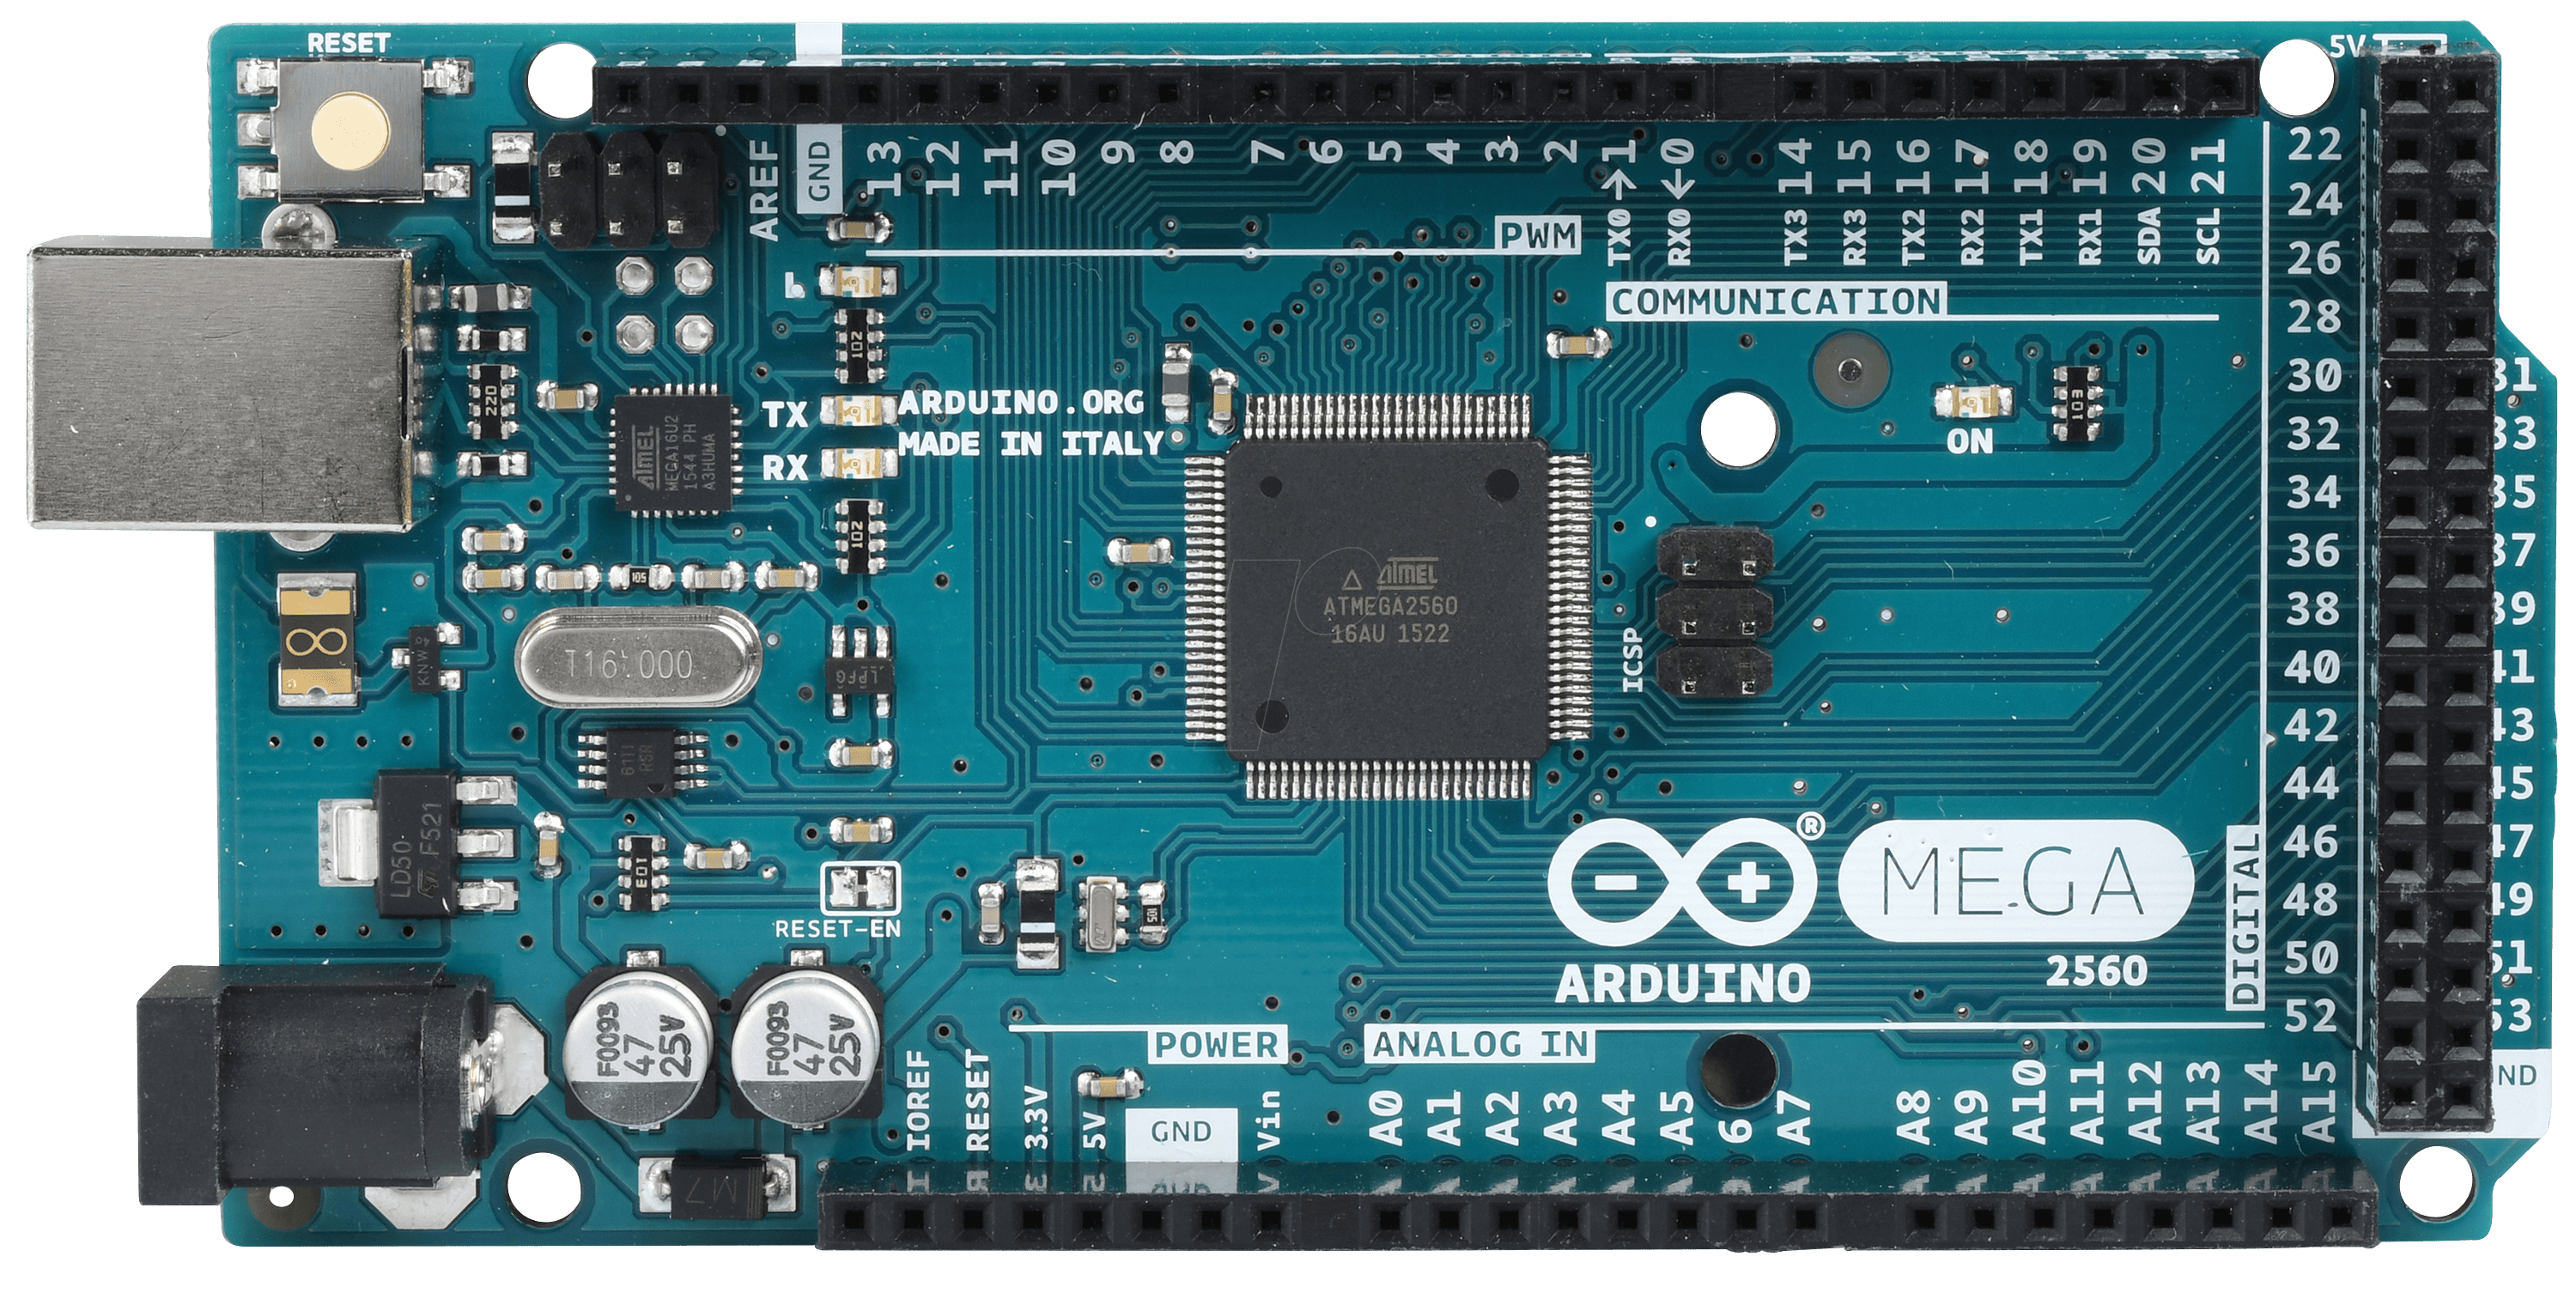
\includegraphics[width=0.5\textwidth]{rysKonstrukcja/Mega.png} & 
				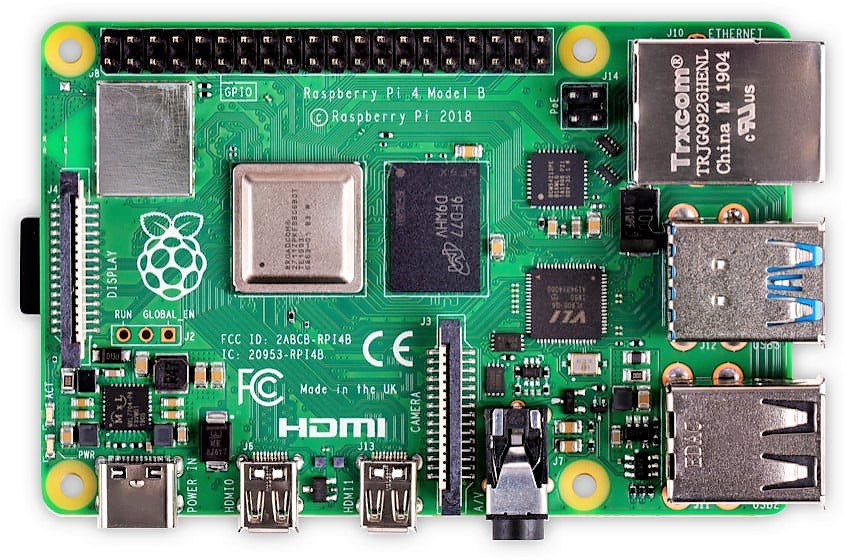
\includegraphics[width=0.5\textwidth]{rysKonstrukcja/raspberry.jpg} \\
			\end{tabular}
			\caption{Mikrokontrolery: a) Arduino Mega, b) Raspberry Pi}
			\label{fig:mikrokontrolery}
		\end{figure}
	
		Trzecią alternatywą łączącą pozytywy obu wymienionych wcześniej platform są mikrokontrolery STM32. Przykładową płytką jest STM32F103 Blue Pill \ref{fig:bluepillPlytka}. Posiada 32 konfigurowalne piny, 16 może obsługiwać zewnętrzne przerwania, 10 pinów połączonych z przetwornikiem ADC. Dodatkowo 18 może pracować z napięciem 5V (sam procesor pracuje na napięciu 3.3V) co może być przydatne zważywszy na fakt, że większa część gotowych modułów pracuje w logice 5V. Procesor wyposażony jest również w kontroler DMA, który pozwala na pomiary ADC oraz komunikację bez użycia procesora. Maksymalna nominalna częstotliwość taktowania wynosi 72MHz i dzięki pętli PLL może być łatwo konfigurowana. W przypadku niewielkiego braku mocy obliczeniowej istnieje możliwość łatwego overclockingu do 128MHz kosztem braku komunikacji przez USB. Procesor wyposażony jest także w 4 timery 16-bitowe, 4-kanałowe. Posiada także kilka możliwości wyboru API. Od wysokopoziomowego STM32duino, opartego na wspomnianym wcześniej Arduino, przez HAL oraz starsze SPL kończąc na systemie czasu rzeczywistego FreeRTOS \cite{FreeRTOS}. Ogromnym plusem jest niska cena. Płytka kosztuje około 1.5\$ (6zł).
	
		\begin{figure}[h]
			\centering
			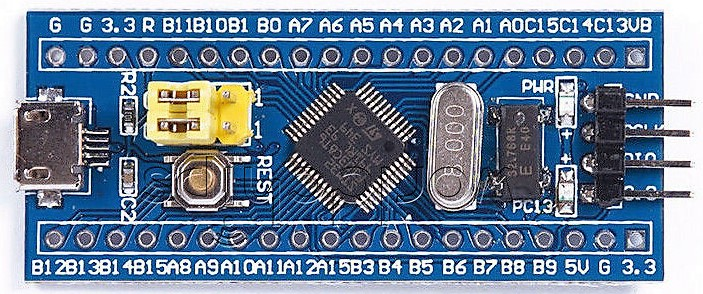
\includegraphics[width=0.8\textwidth]{rysKonstrukcja/bluepill.jpg} 
			\caption{Mikrokontroler STM32F103 Blue Pill}
			\label{fig:bluepillPlytka}
		\end{figure}
		
		Uwzględniając wskazane powyżej informacje wybrano płytkę STM32F103 Blue Pill. Zapewnia doby bilans między ilością peryferiów i wydajnością w porównaniu do pozostałych możliwości. Dodatkowo cechuje się najniższą ceną zakupu.
		
	\section{Pomiar odległości}
		
		Do orientacyjnego pomiaru odległości od przeszkód został wykorzystany moduł z czujnikiem ultradźwiękowym HC-SR04 \ref{fig:HCSR04}. Czujnik pozwala na pomiar odległości w zakresie \SI{2}{} --  \SI{400}{\centi\meter} z rozdzielczością \SI{0.3}{\centi\meter}. W trakcie projektowania brano pod uwagę, że na pomiar wpływa również propagacja fal dźwiękowych. Dlatego uwzględniono dodatkowe czujniki wykrywające przeszkody.
		
		\begin{figure}[H]
			\centering
			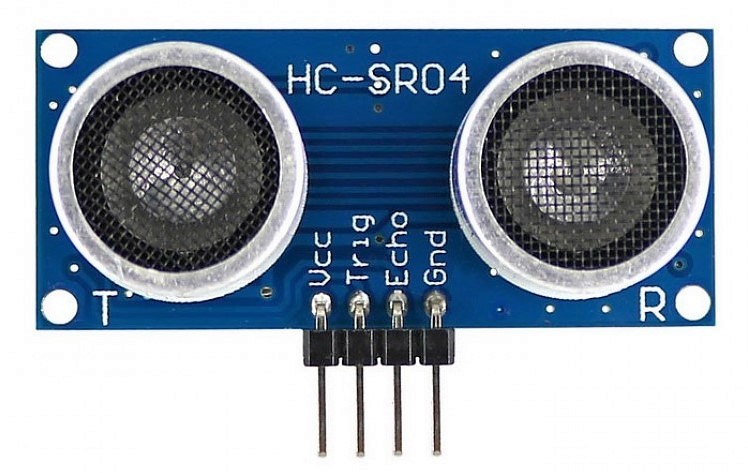
\includegraphics[width=0.4\textwidth]{rysKonstrukcja/HC-SR04.jpg} 
			\caption{Ultradźwiękowy moduł pomiaru odległości}
			\label{fig:HCSR04}
		\end{figure}
	
		Aby dokonać pomiaru czujnikiem należy na wejście Trig podać stan wysoki na co najmniej \SI{10}{\micro\second}. Moduł wysyła wtedy 8 ultradźwiękowych fal o częstotliwości \SI{40}{\kilo\hertz}. Po odebraniu pomiaru na pinie Echo pojawia się stan wysoki. W zależności od odległości od wykrytej przeszkody czas trwania wynosi od \SI{150}{\micro\second} do \SI{22}{\milli\second}. Jeśli nie wykryto przeszkody, czas stanu wysokiego wynosi \SI{38}{\milli\second}. Odległość w centymetrach można obliczyć korzystając z uproszczonej zależności \ref{eq:OdlegloscOdPrzeszkody}.
		
		\begin{equation}\label{eq:OdlegloscOdPrzeszkody}
			d = \unit[\frac{t}{58}]{cm}
		\end{equation}
		gdzie t - czas stanu wysokiego na pinie Echo w \SI{}{\micro\second}.	
		\textcolor{red}{dodać przebiegi z oscyloskopu}
	
	\section{Pomiar odległości od podłogi}
		Aby uniemożliwić robotowi wjazd w niebezpieczny obszar i tym samym zapobiec m.in. spadnięciu ze schodów. Zastosowano czujniki odbiciowe IR mierzące aktualną odległość od podłogi Rys \ref{fig:czujnikIR}. Czujnik ten ma wbudowany komparator LM393 regulowany potencjometrem. W przypadku detekcji zbyt dużej odległości na pin sygnałowy wystawiany jest odpowiedni stan logiczny. Dzięki temu nie ma potrzeby robienia pomiarów ADC oraz obsługi sprzętowej. Pozwala to dzięki mechanizmowi przerwań mikrokontrolera na praktycznie natychmiastową reakcję w przypadku wykrycia niebezpieczeństwa. 
		
		\begin{figure}[H]
			\centering
			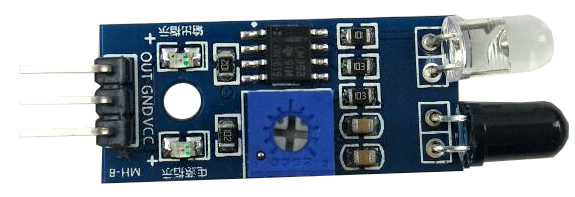
\includegraphics[width=0.6\textwidth]{rys02/czujnikIR.png} 
			\caption{Odbiciowy czujnik IR}
			\label{fig:czujnikIR}
		\end{figure}
	
	\section{Napęd}
		Jako napęd robota wykorzystano silniki szczotkowe DC z wbudowaną przekładnią. Parametry znamionowe silnika przedstawione są w tabeli \ref{tab:Napęd}.
		
		\begin{table}[H]
			\centering
			\begin{tabular}{|l|c|} \hline
				\textbf{Parametr} & Wartość \\
				\hline
				\hline  \textbf{Napięcie zasilania}& 3 -- \SI{6}{\volt}  \\
				\hline 	\textbf{Prędkość obrotowa po redukcji (\SI{6}{\volt})}& \SI{100}{RPM} \\
				\hline 	\textbf{Pobór prądu pod obciążeniem (\SI{6}{\volt})}& \SI{350}{\mA} \\
				\hline 	\textbf{Pobór prądu bez obciążenia (\SI{6}{\volt})}& \SI{170}{\mA} \\
				\hline 	\textbf{Siła ciągu na przekładni (\SI{6}{\volt})}& \SI[per-mode=symbol]{5,5}{\kg\per\cm} \\
				\hline
			\end{tabular}
			\caption{Parametry znamionowe silników napędowych}
			\label{tab:Napęd}
		\end{table}
	
		Do sterowania silnikami wykorzystano mostek H zbudowany w oparciu o układ L9110S. Pozwala on na sterowanie zarówno prędkością jak i kierunkiem obrotów silników niezależnie od siebie. Parametry znamionowe mostka przedstawione są w tabeli \ref{tab:MostekH}.
		
		\begin{table}[H]
			\centering
			\begin{tabular}{|l|c|} \hline
				\textbf{Parametr} & Wartość \\
				\hline
				\hline  \textbf{Napięcie zasilania}& 5 -- \SI{12}{\volt}  \\
				\hline 	\textbf{Maksymalne napięcie zasilania silników} & \SI{12}{\volt} \\
				\hline 	\textbf{Maksymalny prąd na kanał}& \SI{800}{\mA} \\
				\hline 	\textbf{Ilość kanałów}& 2 \\
				\hline 	\textbf{Poziom sygnałów sterujących mostkiem}& CMOS/TTL \\
				\hline
			\end{tabular}
			\caption{Parametry znamionowe mostka H}
			\label{tab:MostekH}
		\end{table}
	
		Sygnały jakie trzeba podać na wejście sterownika aby uzyskać pożądane sterowanie zostały przedstawione w tabeli \ref{tab:tabelaPrawdyMostkaH}.
		
		\begin{table}[H]
			\centering
			\begin{tabular}{|l|c|c|} \hline
				\textbf{1A} & 1B & Stan silnika \\
				\hline
				\hline 	0 & 0 & \textcolor{red}{Hamowanie silnikiem?}\\
				\hline 	1	& 0 & Do przodu \\
				\hline 	0 & 1 & Do tyłu \\
				\hline 	1 & 1 & \textcolor{red}{Hamowanie silnikiem?} \\
				\hline
			\end{tabular}
			\caption{Tabela prawdy mostka H}
			\label{tab:tabelaPrawdyMostkaH}
		\end{table}
		
		Silnik oraz mostek H przedstawione są na rysunku \ref{fig:silnikImostek}
		\begin{figure}[h]
			\centering
			\begin{tabular}{@{}ll@{}}
				a) & b) \\
				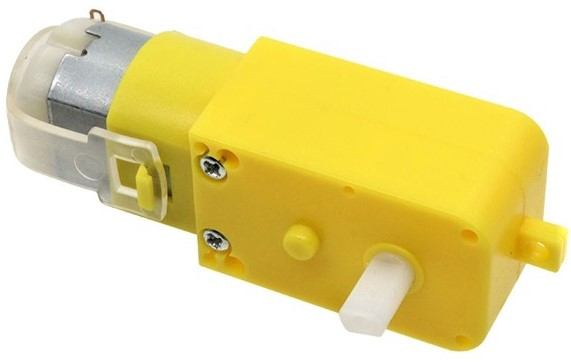
\includegraphics[width=0.5\textwidth]{rys02/silnikDC.jpg} & 
				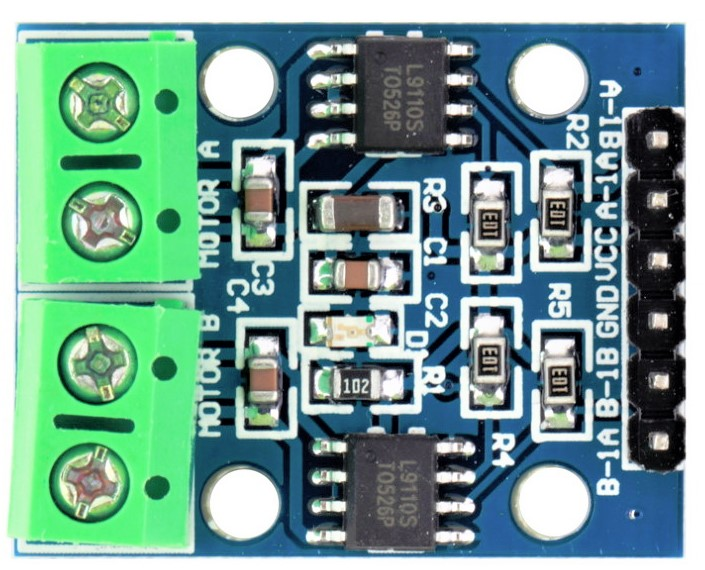
\includegraphics[width=0.4\textwidth]{rys02/mostekHzdj.jpg} \\
			\end{tabular}
			\caption{Zdjęcia: a) Silnika DC, b) Mostka H}
			\label{fig:silnikImostek}
		\end{figure}
	
		Do przeniesienia napędu wykorzystane zostały koła o średnicy \SI{68}{\milli\meter}. Przy maksymalnej prędkości obrotowej silnika robot osiąga prędkość wynoszącą w przybliżeniu \SI[per-mode=symbol]{3.56}{\cm\per\second}.
		
	\section{Rozpoznawanie pozycji}
		Do obliczania aktualnej pozycji i orientacji robota wykorzystanie zostały czujniki szczelinowe w połączeniu z płytkami szczelinowymi. Czujnik optyczny posiada wbudowany komparator LM393 dzięki czemu istnieje prosta możliwość detekcji czy sygnał optyczny jest odbierany czy nie. W połączeniu z płytką szczelinową mocowaną na wale silnika daje to prosty enkoder impulsowy. Płytka szczelinowa posiada rozdzielczość 20 linii na obrót. Obsługując impulsy w przerwaniach mikrokontrolera oraz wyzwalając przerwanie zarówno na zboczu narastającym jak i opadającym można osiągnąć rozdzielczość 40 impulsów na obrót. Uwzględniając średnicę koła niepewność pozycjonowania wynosi w przybliżeniu \SI{5.34}{mm}. Jest ona zbyt duża aby zapewnić precyzyjne sterowanie robotem. Dlatego zdecydowano się na zbudowanie przekładni zwiększającej ilość obrotów płytki enkodera. Przekładnia jest dwustopniowa z 5-krotnym wzmocnieniem w każdym ze stopni. Ostatecznie osiągamy 25-krotne zwiększenie prędkości obrotowej enkodera. Daje to nam 1000 impulsów na obrót i niepewność pozycjonowania wynoszącą w przybliżeniu \SI{0.21}{\milli\meter}. Czujnk szczelinowy wraz z płytką enkodera zostały przedstawione na rysunku \ref{fig:enkoderZplytka}.
		
		\begin{figure}[h]
			\centering
			\begin{tabular}{@{}ll@{}}
				a) & b) \\
				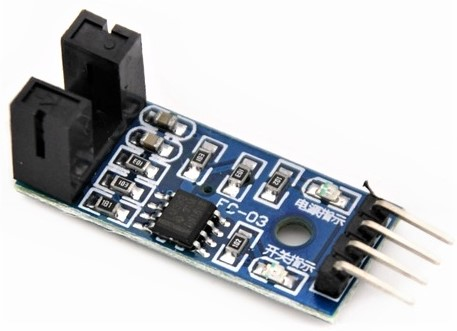
\includegraphics[width=0.5\textwidth]{rys02/enkoder.jpg} & 
				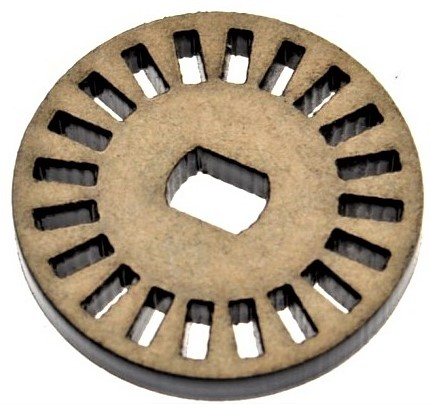
\includegraphics[width=0.2\textwidth]{rys02/plytkaEnkodera.jpg} \\
			\end{tabular}
			\caption{Zdjęcia: a) Czujnik szczelinowy, b) Płytka szczelinowa}
			\label{fig:enkoderZplytka}
		\end{figure}
	
	\section{Zasilanie}
	
		Jako zasilanie wykorzystanie 2 akumulatory Li-Ion 18650 połączone szeregowo. Napięcie nominalne takiego pakietu wynosi \SI{7.4}{\volt}. Przewagą takiego rozwiązania względem połączenia równoległego jest zmniejszenie prądów płynących w przewodach zasilających. Przyczyni się to do mniejszych strat na rezystancjach połączeń oraz zwiększy żywotność przełącznika bistabilnego On/Off. Aby dopasować napięcie do zasilania mikrokontrolera oraz peryferiów wykorzystano 2 przetwornice obniżające napięcie zbudowane w oparciu o układ MP2307. Jedna została wyregulowana na napięcie \SI{3.3}{\volt}, natomiast druga na \SI{5}{\volt}. Parametry techniczne przetwornic zostały przedstawione w tabeli \ref{tab:PrzetwornicaStepDown}.
		
		\begin{table}[H]
			\centering
			\begin{tabular}{|l|c|} \hline
				\textbf{Parametr} & Wartość \\
				\hline
				\hline  \textbf{Napięcie wejściowe}& 4.75 -- \SI{23}{\volt}  \\
				\hline 	\textbf{Napięcie wyjściowe} & 1 -- \SI{17}{\volt} \\
				\hline 	\textbf{Maksymalny prąd wyjściowy}& Szczytowy \SI{3}{\ampere}, ciągły \SI{1.8}{\ampere} \\
				\hline 	\textbf{Maksymalna sprawność konwersji}& \SI{98}{\percent} \\
				\hline 	\textbf{Częstotliwość przełączania}& \SI{340}{\kHz} \\
				\hline
			\end{tabular}
			\caption{Parametry znamionowe przetwornicy obniżającej napięcie}
			\label{tab:PrzetwornicaStepDown}
		\end{table}
	
		Baterie Li-Ion są bardzo wrażliwe zarówno na przeładowywanie \cite{ladowanieLiIon} jak i nadmierne rozładowanie \cite{rozladowywanieLiIon1, rozladowywanieLiIon2}. Najniższe napięcie rozładowania jakiego nie zaleca się przekraczać wynosi \SI{2.4}{\volt}, natomiast typową wartością eksploatacji jest \SI{3}{\volt} \cite{rozladowywanieLiIon2}. Z drugiej strony nadmierne przeładowywanie również drastycznie wpływa na żywotność akumulatorów. Nominalnym napięciem ładowania jest \SI{4.2}{\volt}. Jednak można ładować ogniwa do niższego napięcia zmniejsza się wtedy ich pojemność ale wzrasta żywotność. Wpływ końcowego napięcia ładowania na ogniwa przedstawiono w tabeli w oparciu o informacje ze źródła \cite{ladowanieLiIon}
		
		\begin{table}[H]
			\centering
			\begin{tabular}{|l|c|c|} \hline
				Napięcie końcowe \unit{V} & Ilość cykli rozładowywania & Pojemność ogniwa \\
				\hline
				\hline \SI{4.30}{\volt} & 150 -- 200 & 110 -- \SI{115}{\percent}\\
				\hline \SI{4.25}{\volt}	& 200 -- 350 & 105 -- \SI{110}{\percent}\\
				\hline \SI{4.20}{\volt}	& \textcolor{red}{300 -- 500} & \SI{100}{\percent}\\
				\hline \SI{4.15}{\volt}	& 400 -- 700 & 90 -- \SI{95}{\percent} \\
				\hline \SI{4.10}{\volt}	& 600 -- 1000 & 85 -- \SI{90}{\percent}\\
				\hline \SI{4.05}{\volt} & 850 -- 1500 & 80 -- \SI{85}{\percent}\\
				\hline \SI{4.00}{\volt} & 1200 -- 2000 & 70 -- \SI{75}{\percent}\\
				\hline
			\end{tabular}
			\caption{Wpływ napięcia końcowego na żywotność akumulatorów Li-Ion}
			\label{tab:napięcieKońcoweLiIon}
		\end{table}
	
%%%
%%%Uwaga: tytuł powinien zmieścić się w okienku kolorowej okładki (którą
%%%powinna dostarczyć uczelniana administracja). Proszę posterować
%%%parametrami, aby "wpasować" w okienko własny tekst.
%%%
%%%Do ASAPa należy wprowadzić pracę dyplomową/projekt inżynierski w pliku o nazwie:
%%%
%%%W04_[nr albumu]_[rok kalendarzowy]_[rodzaj pracy] (szczegółowa instrukcja pod adresem asap.pwr.edu.pl)
%%%
           %%%Przykładowo:
        %%%­W04_123456_2015_praca inżynierska.pdf     - praca dyplomowa inżynierska
        %%%W04_123456_2015_projekt inżynierski.pdf   - projekt inżynierski
        %%%W04_123456_2015_praca magisterska.pdf  - praca dyplomowa magisterska
%%%
              %%%rok kalendarzowy ? rok realizacji kursu „Praca dyplomowa” (nie rok obrony) 
\chapter{Testy i symulacje}
    \section{Czas trwania obliczeń}
        W trakcie projektowania sterowania robota warto uwzględnić wydajność obliczeniową mikrokontrolera. Do obliczenia sterowania wymagana jest duża ilość obliczeń zmiennoprzecinkowych. Obliczenia te pochłaniają większą ilość cykli procesora niż obliczenia całkowitoliczbowe. Aby mieć pewność, że obliczenia zostaną wykonane na czas zdecydowano się porównać różnice wynikające z tego faktu. Wzorzec funkcji testującej został przedstawiony w \ref{list:wzorzecCzasTrwania}.
        
        \begin{lstlisting}[label=list:wzorzecCzasTrwania ,caption=Wzorzec funkcji testującej czas wykonywania obliczeń,  basicstyle=\footnotesize\ttfamily]
        template <typename T>
        u32 calculate(T nr1, T nr2) {
            T temp;
            u32 timerStart = micros();
            for(u32 counter{0}; counter < 1000000; ++counter) {
                temp = nr1 * nr2;
                nr1 += temp;
                nr2 += temp + nr1;
            }
            return micros() - timerStart;
        }
        \end{lstlisting}
        Test przeprowadzono dla wbudowanych typów \verb+int+, \verb+float+ oraz \verb+double+. Każdy test został wykonany 5 razy. Wykonano testy z wyłączoną optymalizacją oraz optymalizacją \texttt{-O3}. Wyniki dla flag \texttt{-O0} przedstawiono w tabeli \ref{tab:czasTrwaniaObliczeńO0}.
        
        \begin{table}[ht]
    		\centering
    		\begin{tabular}{|c|c|c|c|}
                \hline
                \multirow{ 2}{*}{\textbf{Numer testu}} & \multicolumn{3}{c|}{\textbf{Czas trwania obliczeń [\si{\milli\second}]}}     \\ \cline{2-4} 
                & \textbf{int} & \textbf{float}   & \textbf{double}      \\ \hline \hline
                1           & 529,446    & 3482,773 & 4332,720     \\ \hline
                2           & 529,470    & 3482,749 & 4332,743     \\ \hline
                3           & 529,467    & 3482,749 & 4332,743     \\ \hline
                4           & 529,469    & 3482,751 & 4332,743     \\ \hline
                5           & 529,467    & 3482,749 & 4332,744     \\ \hline
                \end{tabular}
    		\caption{Czas trwania obliczeń z wyłączoną optymalizacją (flaga O0)}
    		\label{tab:czasTrwaniaObliczeńO0}
    	\end{table}
        Niestety dla optymalizacji prędkości działania za pomocą flagi \texttt{-O3} nie udało się otrzymać wiarygodnych wyników przedstawioną funkcją. Ze względu na uproszczenia jakich dokonał kompilator, niezależnie od ilości powtórzeń pętli otrzymywany wynik wynosi \SI{0}{\micro\second}. Jednak po dodaniu generatora liczb losowych w postaci modyfikacji kodu z \\ 
        \verb+temp = nr1 * nr2;+ \\ 
        na \\
        \verb+temp = nr1 * nr2 * static_cast<T>(random(100000));+ \\ 
        dla wszystkich testów osiągnięto wyniki rzędu \SI{1180}{\milli\second}. Co pozwala twierdzić, że przy użytej optymalizacji kompilator powinien wystarczająco zoptymalizować kod, tak aby nie wynikały z tego powodu znaczne opóźnienia.
        
        Następne porównanie przeprowadzono po implementacji symulacji sterownika kinematycznego w mikrokontrolerze. Porównano maksymalny czas wykonywania jednej pętli dla flag \texttt{-O0}, \texttt{-Os} i~\texttt{-O3}. Wszystkie zmienne, które zawierają części ułamkowe zostały zdefioniowane jako \texttt{double}. Wyniki przedstawiono w tabeli \ref{tab:czasTrwaniaObliczeńSterownik}.
        \begin{table}[ht]
    		\centering
    		\begin{tabular}{|c|c|c|c|}
                \hline
                \multicolumn{4}{|c|}{\textbf{Czas [\si{\micro\second}]}}     \\ \cline{1-4} 
                 \textbf{-O0} & \textbf{-Os}   & \textbf{-O3} & \textbf{-Ofast}       \\ \hline \hline
                   844    & 452 & 450 & 414     \\ \hline
                \end{tabular}
    		\caption{Czas wykonywania jednej pętli w zależności od optymalizacji}
    		\label{tab:czasTrwaniaObliczeńSterownik}
    	\end{table}
    	
    	Dodatkowo porównano wykorzystanie pamięci przez program. Rozmiar pamięci \texttt{RAM} mikrokontrolera to \SI{20480}{B}, natomiast \texttt{Flash} \SI{65536}{B}.
    	\begin{table}[ht]
    		\centering
    		\begin{tabular}{|c|c|c|c|c|}
                \hline
                \multirow{ 2}{*}{\textbf{Pamięć}} & \multicolumn{4}{c|}{\textbf{Wykorzystanie pamięci}}     \\ \cline{2-5} 
                & \textbf{-O0} & \textbf{-Os}   & \textbf{-O3}   & \textbf{-Ofast}     \\ \hline \hline
                 \textbf{RAM}         & \SI{22.9}{\percent} (\SI{4696}{B})   & \SI{22.9}{\percent} (\SI{4680}{B}) & \SI{22.9}{\percent} (\SI{4680}{B}) & \SI{22.9}{\percent} (\SI{4680}{B})     \\ \hline
                 \textbf{Flash}           & \SI{84.6}{\percent} (\SI{55424}{B})    & \SI{59.0}{\percent} (\SI{38688}{B}) & \SI{62.2}{\percent} (\SI{40736}{B})  & \SI{62.2}{\percent} (\SI{40736}{B})     \\ \hline
                \end{tabular}
    		\caption{Wykorzystanie pamięci w zależności od optymalizacji}
    		\label{tab:wykorzystaniePamieciSterownik}
    	\end{table}
    \section{Symulacja działania sterowania kinematycznego}
        Przed właściwą implementacją sterowania kinematycznego zdecydowano się sprawdzić jego zachowanie za pomocą symulacji komputerowej. Do symulacji wykorzystano oprogramowanie \texttt{Matlab} wraz z pakietem \texttt{Simulink}.
    	Wynik działania dla trajektorii kołowej pokazano na rysunku \ref{fig:trajektoriaKolowaWykres}. Parametry $k1$ i~$k2$ to odpowiednio $0.1$ oraz $1$.
    	\begin{figure}[h]
    		\centering
    		\includegraphics[width=0.45\textwidth]{rys03/trajektoriaKoloWykres.eps}
    		\caption{Porównanie trajektorii pochodzącej z generatora oraz robota}
    		\label{fig:trajektoriaKolowaWykres}
    	\end{figure}
    	
    	Następnie zasymulowano dwa różne sposoby generowania trajektorii poruszania się po pomieszczeniu. Parametry $k1$ i~$k2$ pozostały bez zmian. Wyniki przedstawiono na rysunku \ref{fig:porownanieTrajektorii}.
    	\begin{figure}[h]
			\centering
			\begin{tabular}{@{}ll@{}}
				a) & b) \\
				\includegraphics[width=0.45\textwidth]{rys03/trajektoriaRownoleglek1=02k2=10s1.eps} &
				\includegraphics[width=0.45\textwidth]{rys03/trajektoriaKwadratk1=02k2=10s1.eps} 
			\end{tabular}
			\caption{Porównanie dwóch sposobów generowania trajektorii: a) równoległa b) do środka}
			\label{fig:porownanieTrajektorii}
		\end{figure}
		Wynika z nich, że robot ma tendencję do zaokrąglania gwałtownych zmian ruchu. A w przypadku \ref{fig:porownanieTrajektorii} b) co czwarty zakręt następują załamania rzeczywistego ruchu robota. Po zakończeniu generowania trajektorii robot od razu zatrzymuje się w miejscu bez przeregulowań. 
		
		Następnie zdecydowano się na porównać wpływ parametrów $k1$ i~$k2$ na jakość sterowania. Wyniki dla zmian parametru $k1$, przy stałym $k2 = 1$ pokazano na rysunku \ref{fig:porownanieWplywuParametruk1}.
		\begin{figure}[h]
			\centering
			\begin{tabular}{@{}ll@{}}
				a) & b) \\
				\includegraphics[width=0.45\textwidth]{rys03/trajektoriaRownoleglaPorownaniek1.eps} &
				\includegraphics[width=0.45\textwidth]{rys03/trajektoriaKwadratPorownaniek1.eps}
			\end{tabular}
			\caption{Porównanie wpływu parametru k1 na trajektorię: a) równoległą b) do środka}
			\label{fig:porownanieWplywuParametruk1}
		\end{figure}
		Można z nich wnioskować, że parametr ten ma wpływ na przeregulowania podczas zmian trajektorii. Gdy jest zbyt mały, robot skraca zakręty. Natomiast wraz z~jego wzrostem, robot ma tendencję do coraz większego zaokrąglania zakrętów. Przy dużych wartościach, powstaje także przeregulowanie na prostym odcinku drogi.  
		
		Wyniki dla zmian parametru $k2$, przy stałym $k1=0.1$ zostały przedstawione na rysunku \ref{fig:porownanieWplywuParametruk2}.
		\begin{figure}[h]
			\centering
			\begin{tabular}{@{}ll@{}}
				a) & b) \\
				\includegraphics[width=0.45\textwidth]{rys03/trajektoriaRownoleglaPorownaniek2.eps} &
				\includegraphics[width=0.45\textwidth]{rys03/trajektoriaKwadratPorownaniek2.eps}
			\end{tabular}
			\caption{Porównanie wpływu parametru k2 na trajektorię: a) równoległą b) do środka}
			\label{fig:porownanieWplywuParametruk2}
		\end{figure}
    	Zwiększenie tego parametru powoduje poprawę jakości podążania za zadaną trajektorią. Gdy jest zbyt mały, robot zbyt wcześnie zawraca i następują załamania trajektorii w przypadku trajektorii równoległej. Natomiast w~przypadku trajektorii do środka, następuje zaokrąglenie zakrętów.
    	
    	Znając wpływ parametrów $k1$ i~$k2$ można dobrać ich wartości do robota. Aby było to możliwe należy sprawdzić prędkości obrotowe kół. Powinny być możliwe do zrealizowania przez silniki. Jako parametry testowe wybrano $k1 = 1$ oraz $k2 = 10$. Prędkość postępowa robota wynosi \SI[per-mode=symbol]{1}{\metre\per\second}.
    	\begin{figure}[h]
			\centering
			\begin{tabular}{@{}ll@{}}
				a) & b) \\
				\includegraphics[width=0.45\textwidth]{rys03/trajektoriaRownoleglek1=1k2=10.eps} &
				\includegraphics[width=0.45\textwidth]{rys03/predkosciKolRownoleglek1=1k2=10.eps}
			\end{tabular}
			\caption{Zestawienie: a) Trajektoria równoległa b) Prędkości kół}
			\label{fig:trajektoriaRownoleglaIPredkoscKolk1=1k2=10}
		\end{figure}
		\begin{figure}[h]
			\centering
			\begin{tabular}{@{}ll@{}}
				a) & b) \\
				\includegraphics[width=0.45\textwidth]{rys03/trajektoriaKwadratk1=1k2=10.eps} &
				\includegraphics[width=0.45\textwidth]{rys03/predkosciKolKwadratk1=1k2=10.eps}
			\end{tabular}
			\caption{Zestawienie: a) Trajektoria do środka b) Prędkości kół}
			\label{fig:trajektoriaKwadratIPredkoscKolk1=1k2=10}
		\end{figure}
		Dla obu trajektorii \ref{fig:trajektoriaRownoleglaIPredkoscKolk1=1k2=10} i~\ref{fig:trajektoriaKwadratIPredkoscKolk1=1k2=10} prędkości obrotowe kół dla odcinków prostych wynoszą $\approx~\SI[per-mode=symbol]{4.7}{obr\per\second}$. Natomiast zastosowane silniki według dokumentacji pozwalają na osiągnięcie $\SI[per-mode=symbol]{100}{obr\per\min} = 1\SI[per-mode=symbol, quotient-mode=fraction]{2/3}{obr\per\second}$. Oznacza to, że robot nie jest w stanie poruszać się z taką prędkością. Dodatkowo na zakrętach odnotowywane są skoki prędkości obrotowych. W~przypadku \ref{fig:trajektoriaKwadratIPredkoscKolk1=1k2=10}b) co czwarty zakręt dochodzi do przeregulowań i gwałtownych skoków prędkości obrotowych.
		
		W pierwszej kolejności zdecydowano się zmniejszyć prędkość postępową robota do \SI[per-mode=symbol]{10}{\centi\metre\per\second}. Zmodyfikowano także trajektorię, tak aby odpowiadała szerokości szczotek myjących podłogę.
		\begin{figure}[h]
			\centering
			\begin{tabular}{@{}ll@{}}
				a) & b) \\
				\includegraphics[width=0.45\textwidth]{rys03/trajektoriaRownoleglek1=1k2=10s=01d02.eps} &
				\includegraphics[width=0.45\textwidth]{rys03/predkoscKolRownoleglek1=1k2=10s=01d02.eps}
			\end{tabular}
			\caption{Zestawienie dla prędkości \SI[per-mode=symbol]{10}{\centi\metre\per\second}: a) Trajektoria równoległa b) Prędkości kół}
			\label{fig:trajektoriaRownolegleIPredkoscKolk1=1k2=10s=01d=02}
		\end{figure}
		\begin{figure}[h]
			\centering
			\begin{tabular}{@{}ll@{}}
				a) & b) \\
				\includegraphics[width=0.45\textwidth]{rys03/trajektoriaKwadratk1=1k2=10d02s01.eps} &
				\includegraphics[width=0.45\textwidth]{rys03/predkosciKolKwadratk1=1k2=10d02s01.eps}
			\end{tabular}
			\caption{Zestawienie dla prędkości \SI[per-mode=symbol]{10}{\centi\metre\per\second}: a) Trajektoria do środka b) Prędkości kół}
			\label{fig:trajektoriaKwadratIPredkoscKolk1=1k2=10s=01d=02}
		\end{figure}
		Jak pokazuje rysunek \ref{fig:trajektoriaRownolegleIPredkoscKolk1=1k2=10s=01d=02} i \ref{fig:trajektoriaKwadratIPredkoscKolk1=1k2=10s=01d=02}. Prędkość obrotowa na odcinkach prostych zgodnie z oczekiwaniami spadła dziesięciokrotnie do poziomu $\approx~\SI[per-mode=symbol]{0.45}{obr\per\second}$ i~mieści się w możliwym do zrealizowania przez silniki przedziale. Natomiast osłabieniu nie uległy prędkości obrotowe kół podczas załamań trajektorii i nadal znacznie przekraczają dopuszczalne przez silniki prędkości. Z tego powodu postanowiono ustawić limity prędkości obrotowych kół w modelu i~sprawdzić ich wpływ na zachowanie robota. Wyniki przedstawiają rysunki \ref{fig:trajektoriaRownolegleIPredkoscKolk1=1k2=10s=01d=02Limit} i~\ref{fig:trajektoriaKwadratIPredkoscKolk1=1k2=10s=01d=02Limit}.
		\begin{figure}[h]
			\centering
			\begin{tabular}{@{}ll@{}}
				a) & b) \\
				\includegraphics[width=0.45\textwidth]{rys03/trajektoriaRownoleglek1=1k2=10s=01d02Limit.eps} &
				\includegraphics[width=0.45\textwidth]{rys03/predkoscKolRownoleglek1=1k2=10s=01d02Limit.eps}
			\end{tabular}
			\caption{Zestawienie z limitem prędkości kół: a) Trajektoria równoległa b) Prędkości kół}
			\label{fig:trajektoriaRownolegleIPredkoscKolk1=1k2=10s=01d=02Limit}
		\end{figure}
		\begin{figure}[h]
			\centering
			\begin{tabular}{@{}ll@{}}
				a) & b) \\
				\includegraphics[width=0.45\textwidth]{rys03/trajektoriaKwadratk1=1k2=10d02s01Limit.eps} &
				\includegraphics[width=0.45\textwidth]{rys03/predkosciKolKwadratk1=1k2=10d02s01Limit.eps}
			\end{tabular}
			\caption{Zestawienie z limitem prędkości kół: a) Trajektoria do środka b) Prędkości kół}
			\label{fig:trajektoriaKwadratIPredkoscKolk1=1k2=10s=01d=02Limit}
		\end{figure}
		Widać na nich pogorszenie jakości śledzenia trajektorii. Natomiast maksymalne prędkości kół mieszczą się w zakresie realizowanym przez silniki. 
		
		Uwzględniając wszystkie badania można stwierdzić, że kluczowym problemem wprowadzającym błędy do układu są gwałtowne zmiany trajektorii. Dlatego na zakrętach postanowiono wygenerować trajektorię po łuku i sprawdzić wpływ tej zmiany na jakość śledzenia trajektorii.
		\begin{figure}[h]
			\centering
			\begin{tabular}{@{}ll@{}}
				a) & b) \\
				\includegraphics[width=0.45\textwidth]{rys03/trajektoriaRownoleglek1=1k2=10s=01d02LimitZaokraglone.eps} &
				\includegraphics[width=0.45\textwidth]{rys03/predkoscKolRownoleglek1=1k2=10s=01d02LimitZaokraglone.eps}
			\end{tabular}
			\caption{Zestawienie po modyfikacjitrajektorii: a) Trajektoria równoległa b) Prędkości kół}
			\label{fig:trajektoriaRownolegleIPredkoscKolk1=1k2=10s=01d=02LimitZaokraglone}
		\end{figure}
		\begin{figure}[h]
			\centering
			\begin{tabular}{@{}ll@{}}
				a) & b) \\
				\includegraphics[width=0.45\textwidth]{rys03/trajektoriaKwadratk1=1k2=10d02s01LimitZaokraglone.eps} &
				\includegraphics[width=0.45\textwidth]{rys03/predkosciKolKwadratk1=1k2=10d02s01LimitZaokraglone.eps}
			\end{tabular}
			\caption{Zestawienie po modyfikacji trajektorii: a) Trajektoria do środka b) Prędkości kół}
			\label{fig:trajektoriaKwadratIPredkoscKolk1=1k2=10s=01d=02LimitZaokrąglone}
		\end{figure}
		Zmniejszenie gwałtownych zmian trajektorii pozwala także dobrać wyższe wartości parametrów $k1$ i~$k2$. Wyniki dla $k1 = 10, k2 = 100$ przedstawiają rysunki \ref{fig:trajektoriaRownolegleIPredkoscKolk1=1k2=10s=01d=02LimitZaokraglone} oraz \ref{fig:trajektoriaKwadratIPredkoscKolk1=1k2=10s=01d=02LimitZaokrąglone}. Po wprowadzonych zmianach w przypadku trajektorii równoległej jakość realizowanej przez robota trajektorii jest zadowalająca, a~prędkości obrotowe kół maksymalnie wynoszą $\approx\SI[per-mode=symbol]{1}{obr\per\second}$ i~mieszczą się w zakresie realizowanym przez silniki z dodatkowym marginesem błędu. Natomiast w przypadku trajektorii do środka rezultat jest nieco gorszy, ale maksymalne prędkości obrotowe kół są o połowę mniejsze niż w trajektorii równoległej. 
		
		Na wszystkich symulacjach dla trajektorii do środka można zauważyć charakterystyczne przeregulowania podczas zmiany kąta obrotu z $\frac{3}{2}\pi$ do $2\pi$. Aby zbadać to zjawisko postanowiono porównać wartości kątów pochodzących z generatora oraz obiektu. Porównanie zostało pokazane na rysunku \ref{fig:katyKwadrat}.
		\begin{figure}[ht]
			\centering
				\includegraphics[width=0.45\textwidth]{rys03/katyKwadratk1=1k2=10d02s01LimitZaokraglone.eps} 
			\caption{Porównanie kątów obrotu z generatora i~obiektu}
			\label{fig:katyKwadrat}
		\end{figure}
		Można z niego wnioskować, że robot zamiast osiągnąć pełny kąt $2\pi$ czyli wartość początkową $0$, obraca się w drugą stronę i~tak osiąga ten kąt. To w~połączeniu z ograniczeniami prędkości kół powoduje przedstawiony efekt. Aby rozwiązać ten problem postanowiono zmienić zakres matematycznego zapisu kąta obrotu robota. Zakres $\langle 0, 2\pi)$ rozszerzono do $(-\infty, +\infty)$. Pozwoli to przechowywać pełną informację o ilości obrotów robota i rozwiąże problem powracania do pozycji początkowej. W rzeczywistej implementacji robota zakres ten będzie ograniczony do wartości brzegowych zmiennych w zależności od użytego typu. Trajektoria po wprowadzonej zmianie, wraz z prędkościami kół przedstawiono na rys 
        \ref{fig:trajektoriaKwadratPredkosciKoliKatyZaokrągloneNaprawione}.
		\begin{figure}[ht]
			\centering
			\begin{tabular}{@{}ll@{}}
				a) & b) \\
				\includegraphics[width=0.45\textwidth]{rys03/trajektoriaKwadratk1=1k2=10d02s01LimitZaokragloneNaprawione.eps} &
				\includegraphics[width=0.45\textwidth]{rys03/predkosciKolKwadratk1=1k2=10d02s01LimitZaokragloneNaprawione.eps}
			\end{tabular}
			\caption{Wpływ modyfikacji zakresu kątów na: a) Trajektorię b) Prędkości kół}
			\label{fig:trajektoriaKwadratPredkosciKoliKatyZaokrągloneNaprawione}
		\end{figure}
		Widać na nich, że nie występują już charakterystyczne przeregulowania.
		
		Następnie zaimplementowano sterownik kinematyczny bezpośrednio w~mikrokontrolerze. Z~uwagi na wykorzystany framework \texttt{stm32duino} oraz język \texttt{C++} w standardzie \texttt{C++11}, zdecydowano się na podejście obiektowe. Do celów wizualizacji trajektorii w czasie rzeczywistym postanowiono wykorzystać środowisko \texttt{Processing} oparte o język \texttt{Java}. Dodatkowo dane są logowane do pliku \texttt{txt} i~wyświetlane za pomocą skryptu w języku \texttt{Python} oraz biblioteki \texttt{Matplotlib}. Co umożliwia późniejszą interpretację danych. Czas powtarzania pętli został ustawiony na \SI{10}{\milli\second}, co daje aktualizację pozycji z częstotliwością \SI[per-mode=symbol]{100}{powtórzeń\per\second}.
		Trajektoria z podglądu w środowisku \texttt{Processing} została pokazana na rysunku \ref{fig:trajektoriaProcessing}. Parametry symulacji ustawiono na $k1 = 1$, $k2 = 1$. Kolor biały reprezentuje trajektorię zadaną, natomiast czerwony rzeczywistą.
		\begin{figure}[ht]
			\centering
				\includegraphics[width=0.45\textwidth]{rys03/trajektoriaProcessingk1=1k2=1.png} 
			\caption{Trajektoria rysowana w środowisku Processing}
			\label{fig:trajektoriaProcessing}
		\end{figure}
		Następnie wyrysowano szczegółowe informacje zawarte w pliku \texttt{.txt}. Wyniki zostały przedstawione na rysunkach \ref{fig:predkosciPython} oraz \ref{fig:kolaiKatPython}.
		\begin{figure}[ht]
			\centering
			\begin{tabular}{@{}ll@{}}
				a) & b) \\
				\includegraphics[width=0.45\textwidth]{rys03/predkosciLinowePythonk1=1k2=2.eps} &
				\includegraphics[width=0.45\textwidth]{rys03/predkosciKatkowePythonk1=1k2=2.eps}
			\end{tabular}
			\caption{Prędkości robota: a) Liniowa b) Kątowa}
			\label{fig:predkosciPython}
		\end{figure}
		\begin{figure}[ht]
			\centering
			\begin{tabular}{@{}ll@{}}
				a) & b) \\
				\includegraphics[width=0.45\textwidth]{rys03/predkosciKolPythonk1=1k2=2.eps} &
				\includegraphics[width=0.45\textwidth]{rys03/katObrotuPythonk1=1k2=2.eps}
			\end{tabular}
			\caption{a) Prędkości kół b) Kąt obrotu}
			\label{fig:kolaiKatPython}
		\end{figure}
		Uzyskane wyniki są podobne do tych ze środowiska \texttt{Matlab/Simulink}.
    \section{Drgania styków}
    Dla układów stykowych takich jak przyciski, przełączniki etc. istnieje zjawisko drgań styków. Pojawia się ono przy niepełnym kontakcie styków w trakcie włączania/wyłączania i potrafi trwać do \SI{20}{\milli\second} \textcolor{red}{dodać źródło}. Zjawisko to powoduje wielokrotne odczyty kliknięć przez mikrokontroler pojedynczej zmiany stany przycisku. Jednym z rozwiązań sprzętowych jest dodanie filtru RC o odpowiedniej stałej czasowej. Przykład drgań styków oraz zastosowania filtru został przedstawiony na rysunku \ref{fig:drganiaStykow}.
        \begin{figure}[ht]
			\centering
			\begin{tabular}{@{}ll@{}}
				a) & b) \\
				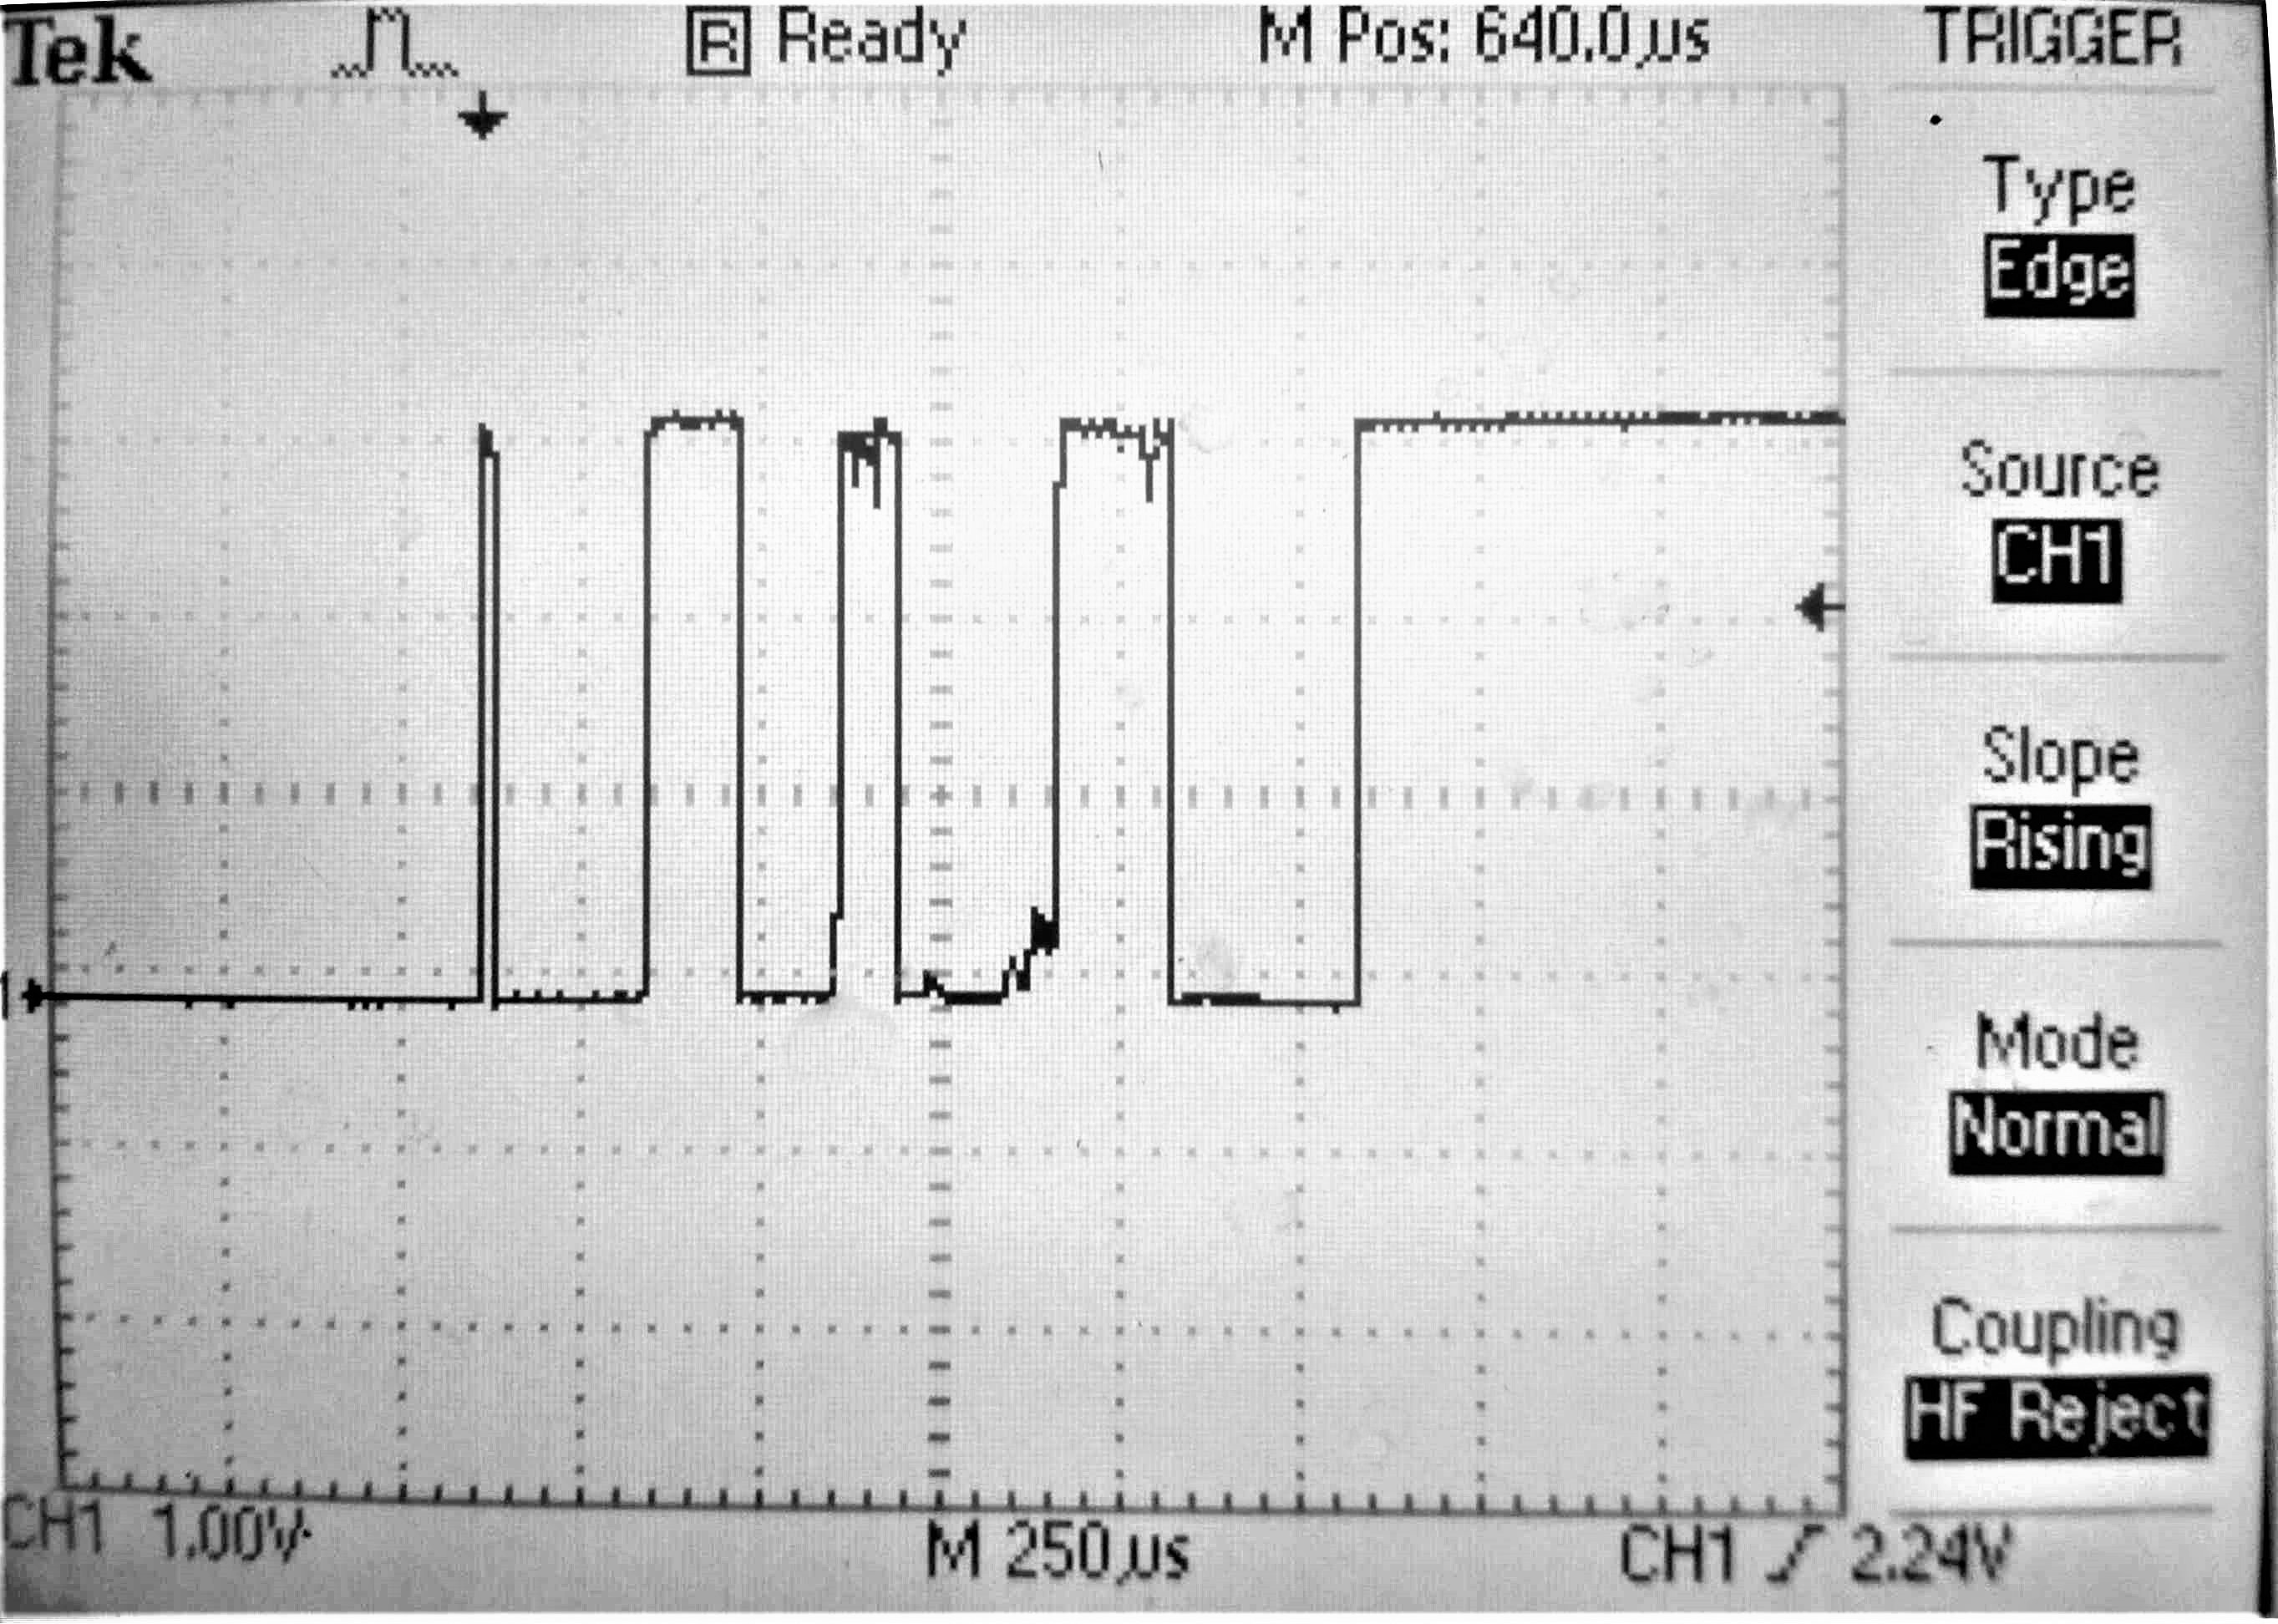
\includegraphics[width=0.45\textwidth]{rys03/drganiaPrzyciskow.jpg} & 
				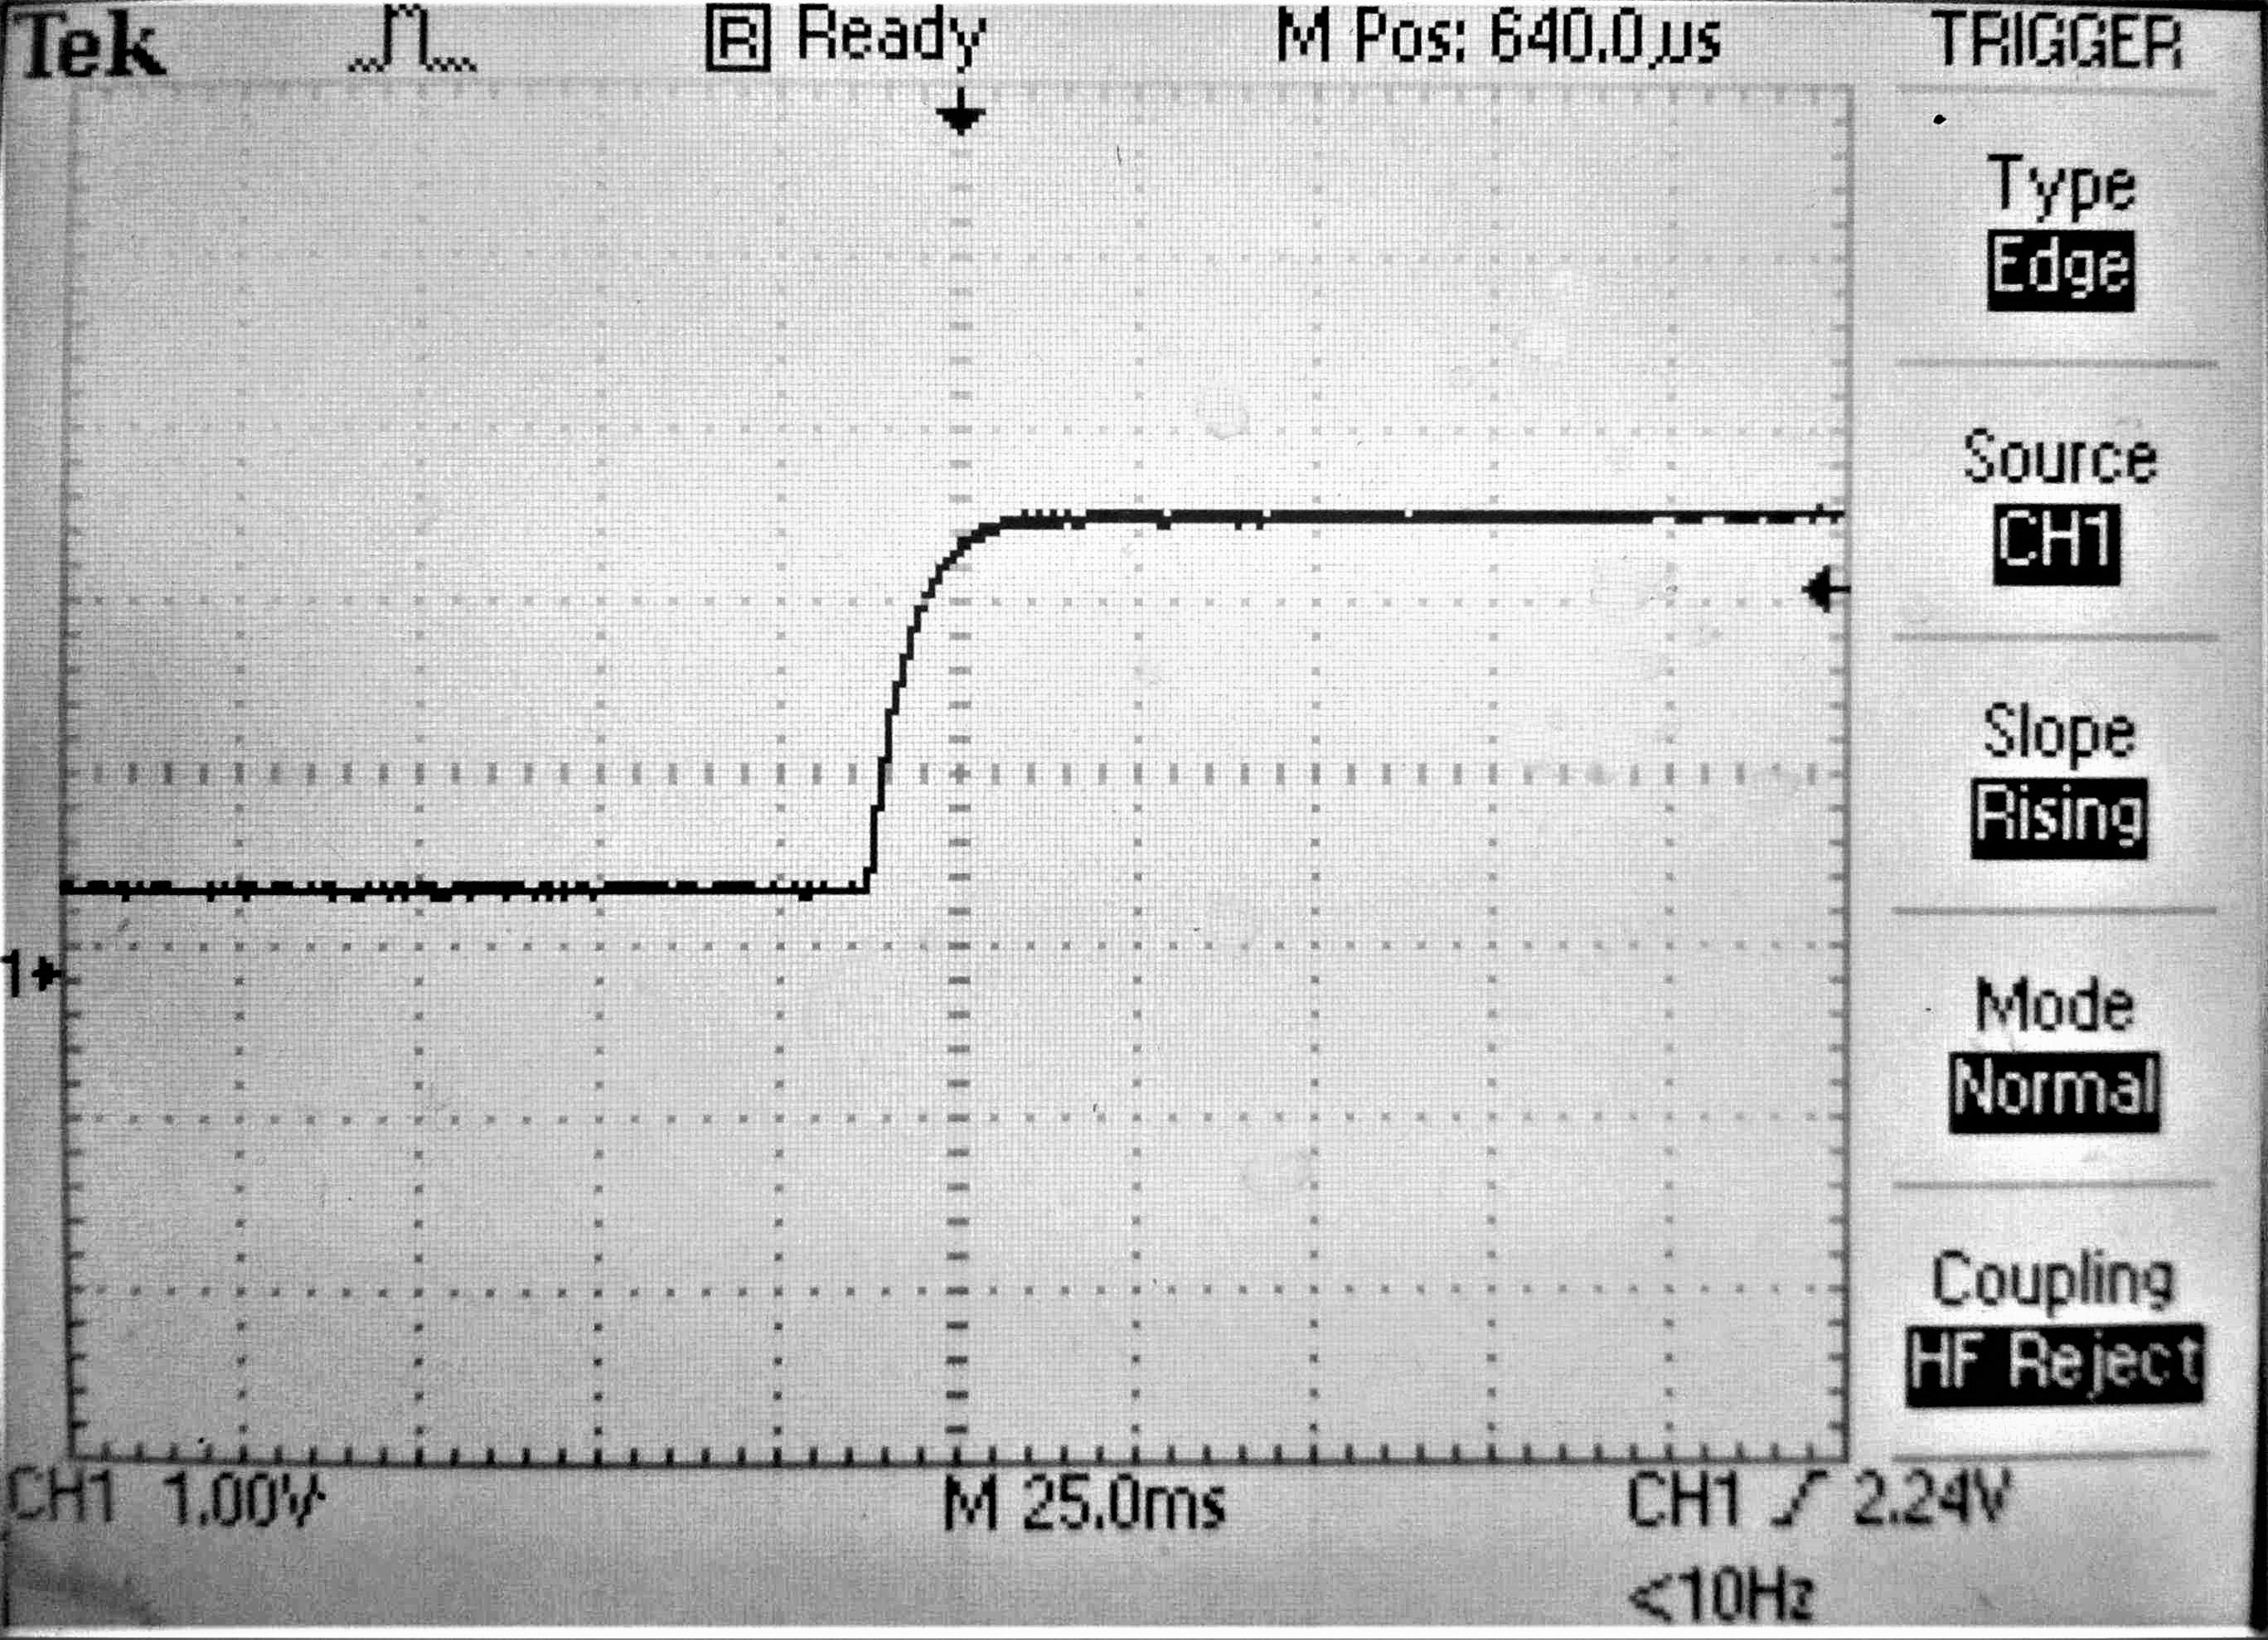
\includegraphics[width=0.45\textwidth]{rys03/drganiaStykowFiltr.jpg} \\
			\end{tabular}
			\caption{Drania styków a) przed filtracją b) po filtracji}
			\label{fig:drganiaStykow}
		\end{figure}
		
	\section{Filtracja zasilania}
    	Przetwornice DC-DC na wyjściu posiadają pewne nierówności zasilania. Dlatego warto zastosować filtrację w postaci dławików i kondensatorów. Badania przeprowadzono dla przetwornicy obniżającej napięcie MP2307. Do filtracji użyto dławika \textcolor{red}{wartość} oraz kondensatora \SI{2200}{\micro\farad}.
	    \begin{figure}[ht]
			\centering
			\begin{tabular}{@{}ll@{}}
				a) & b) \\
				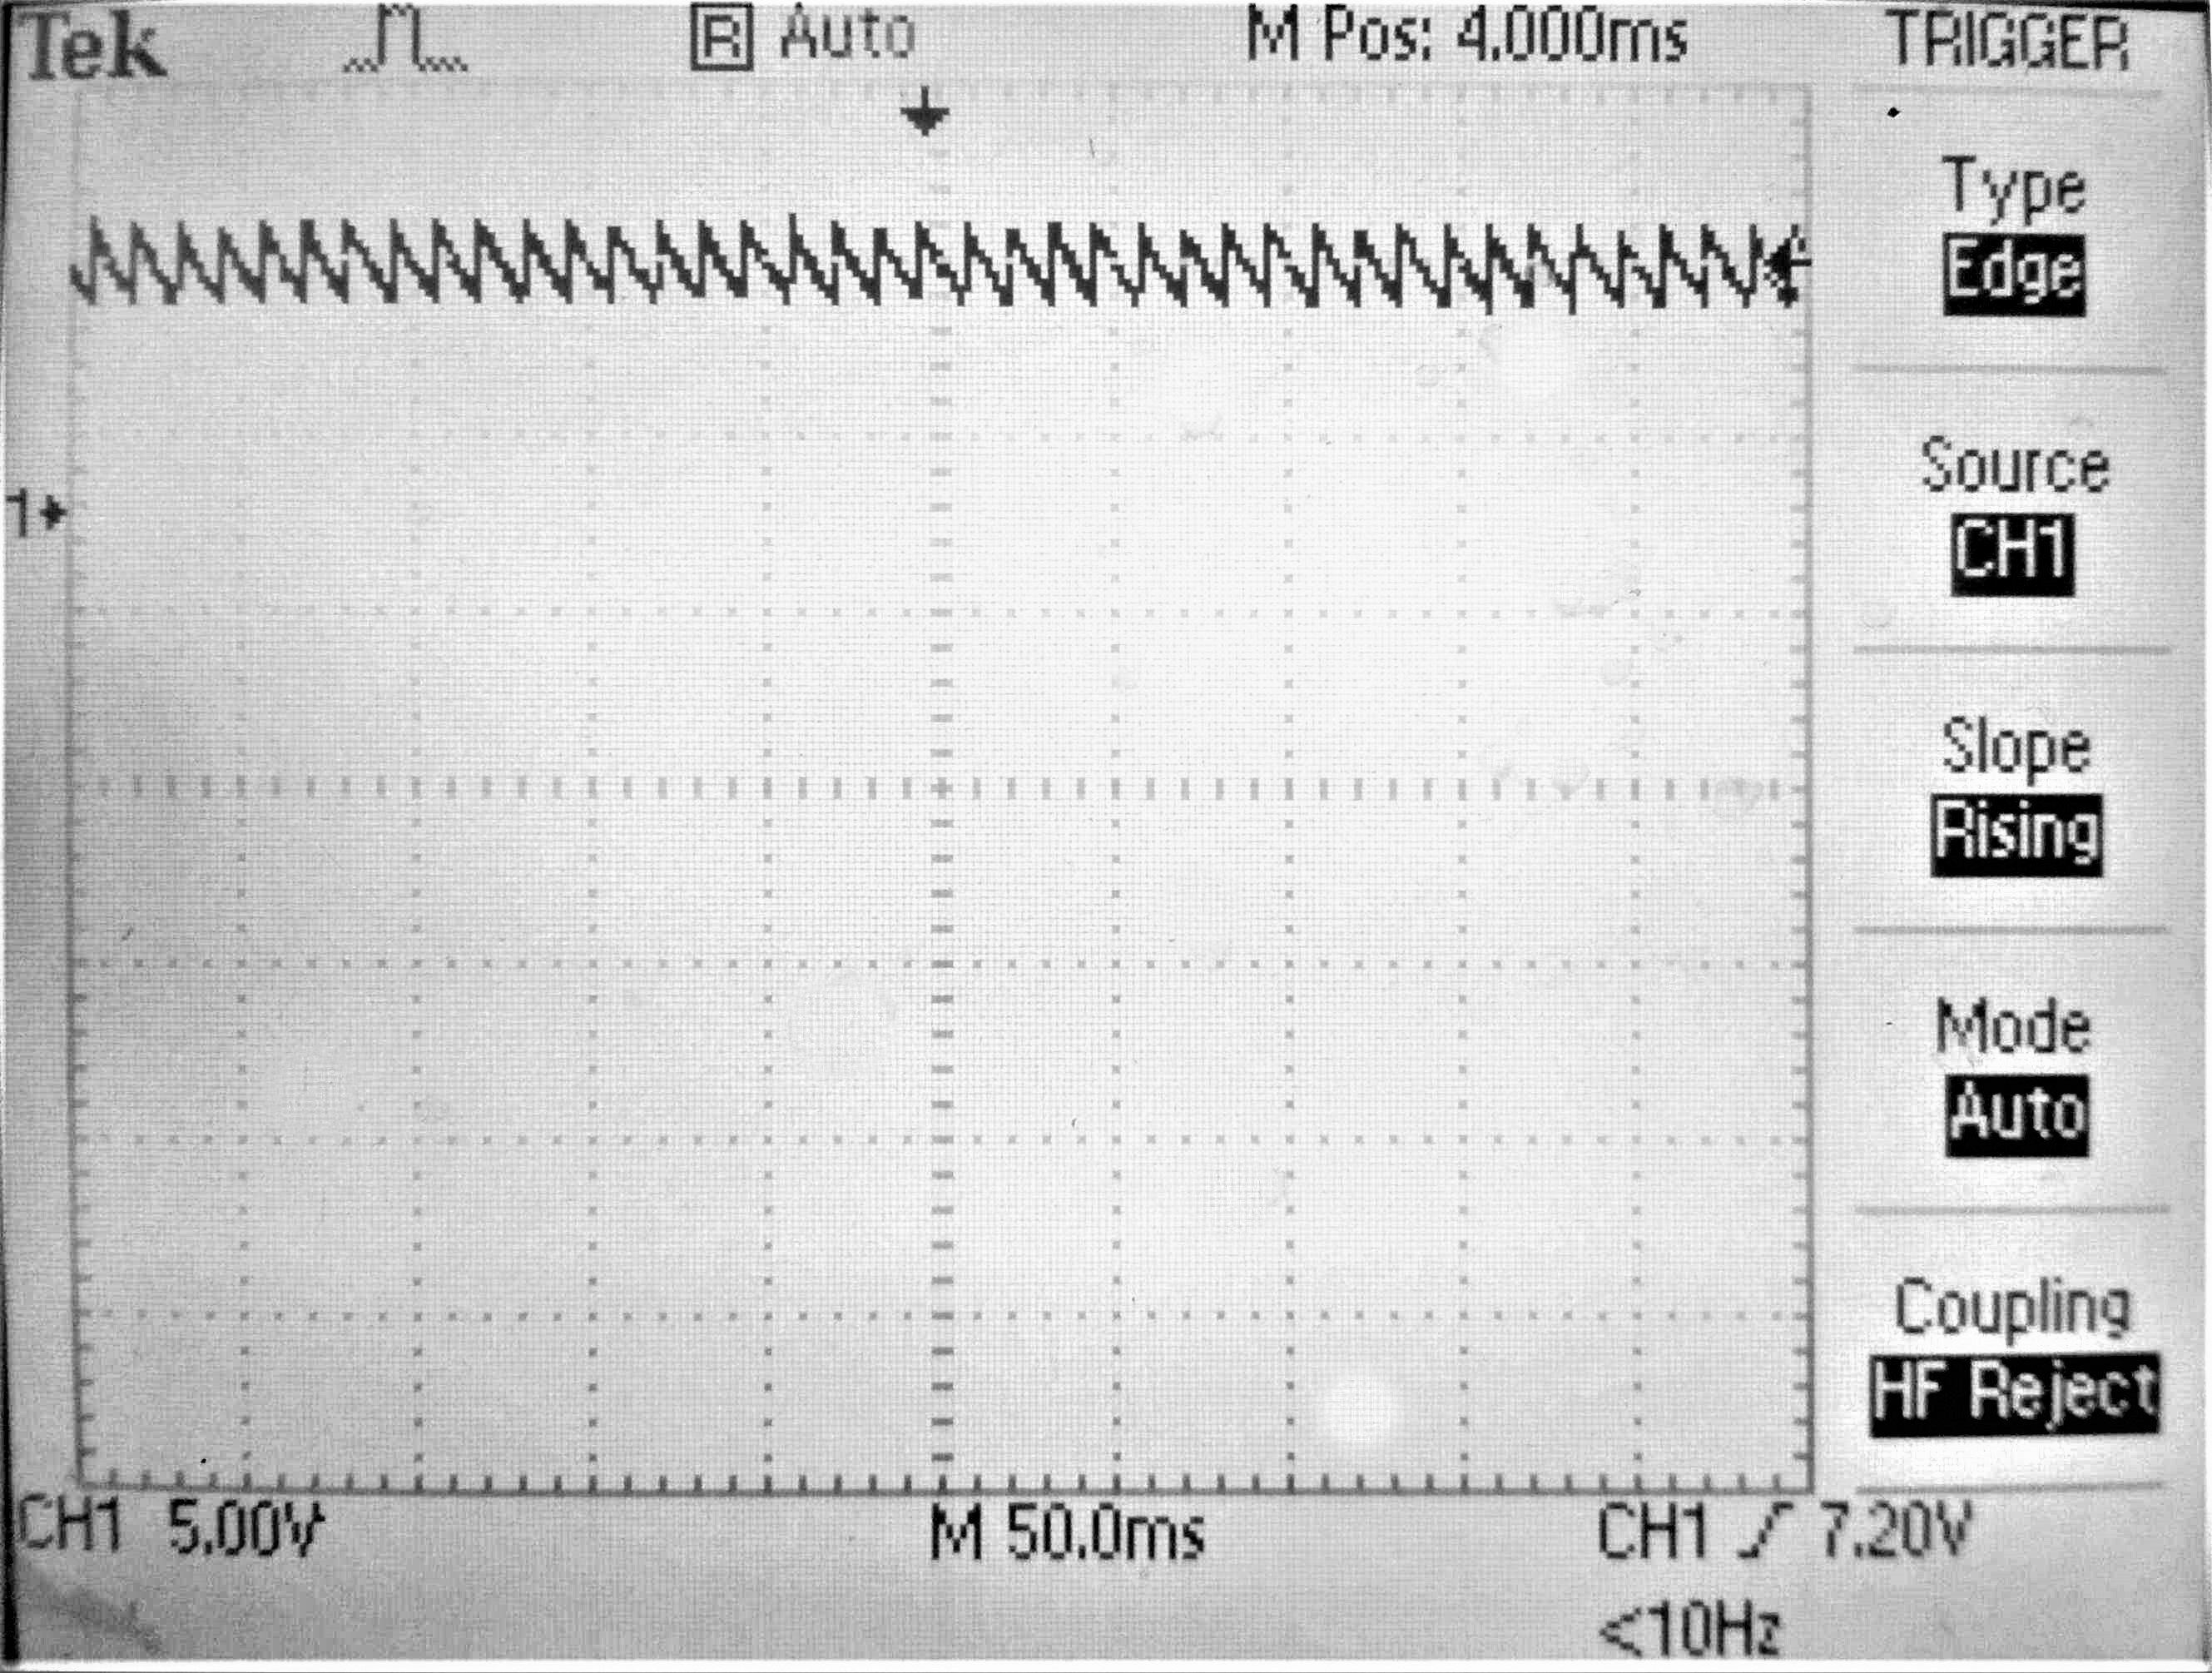
\includegraphics[width=0.45\textwidth]{rys03/zasilanie.jpg} & 
				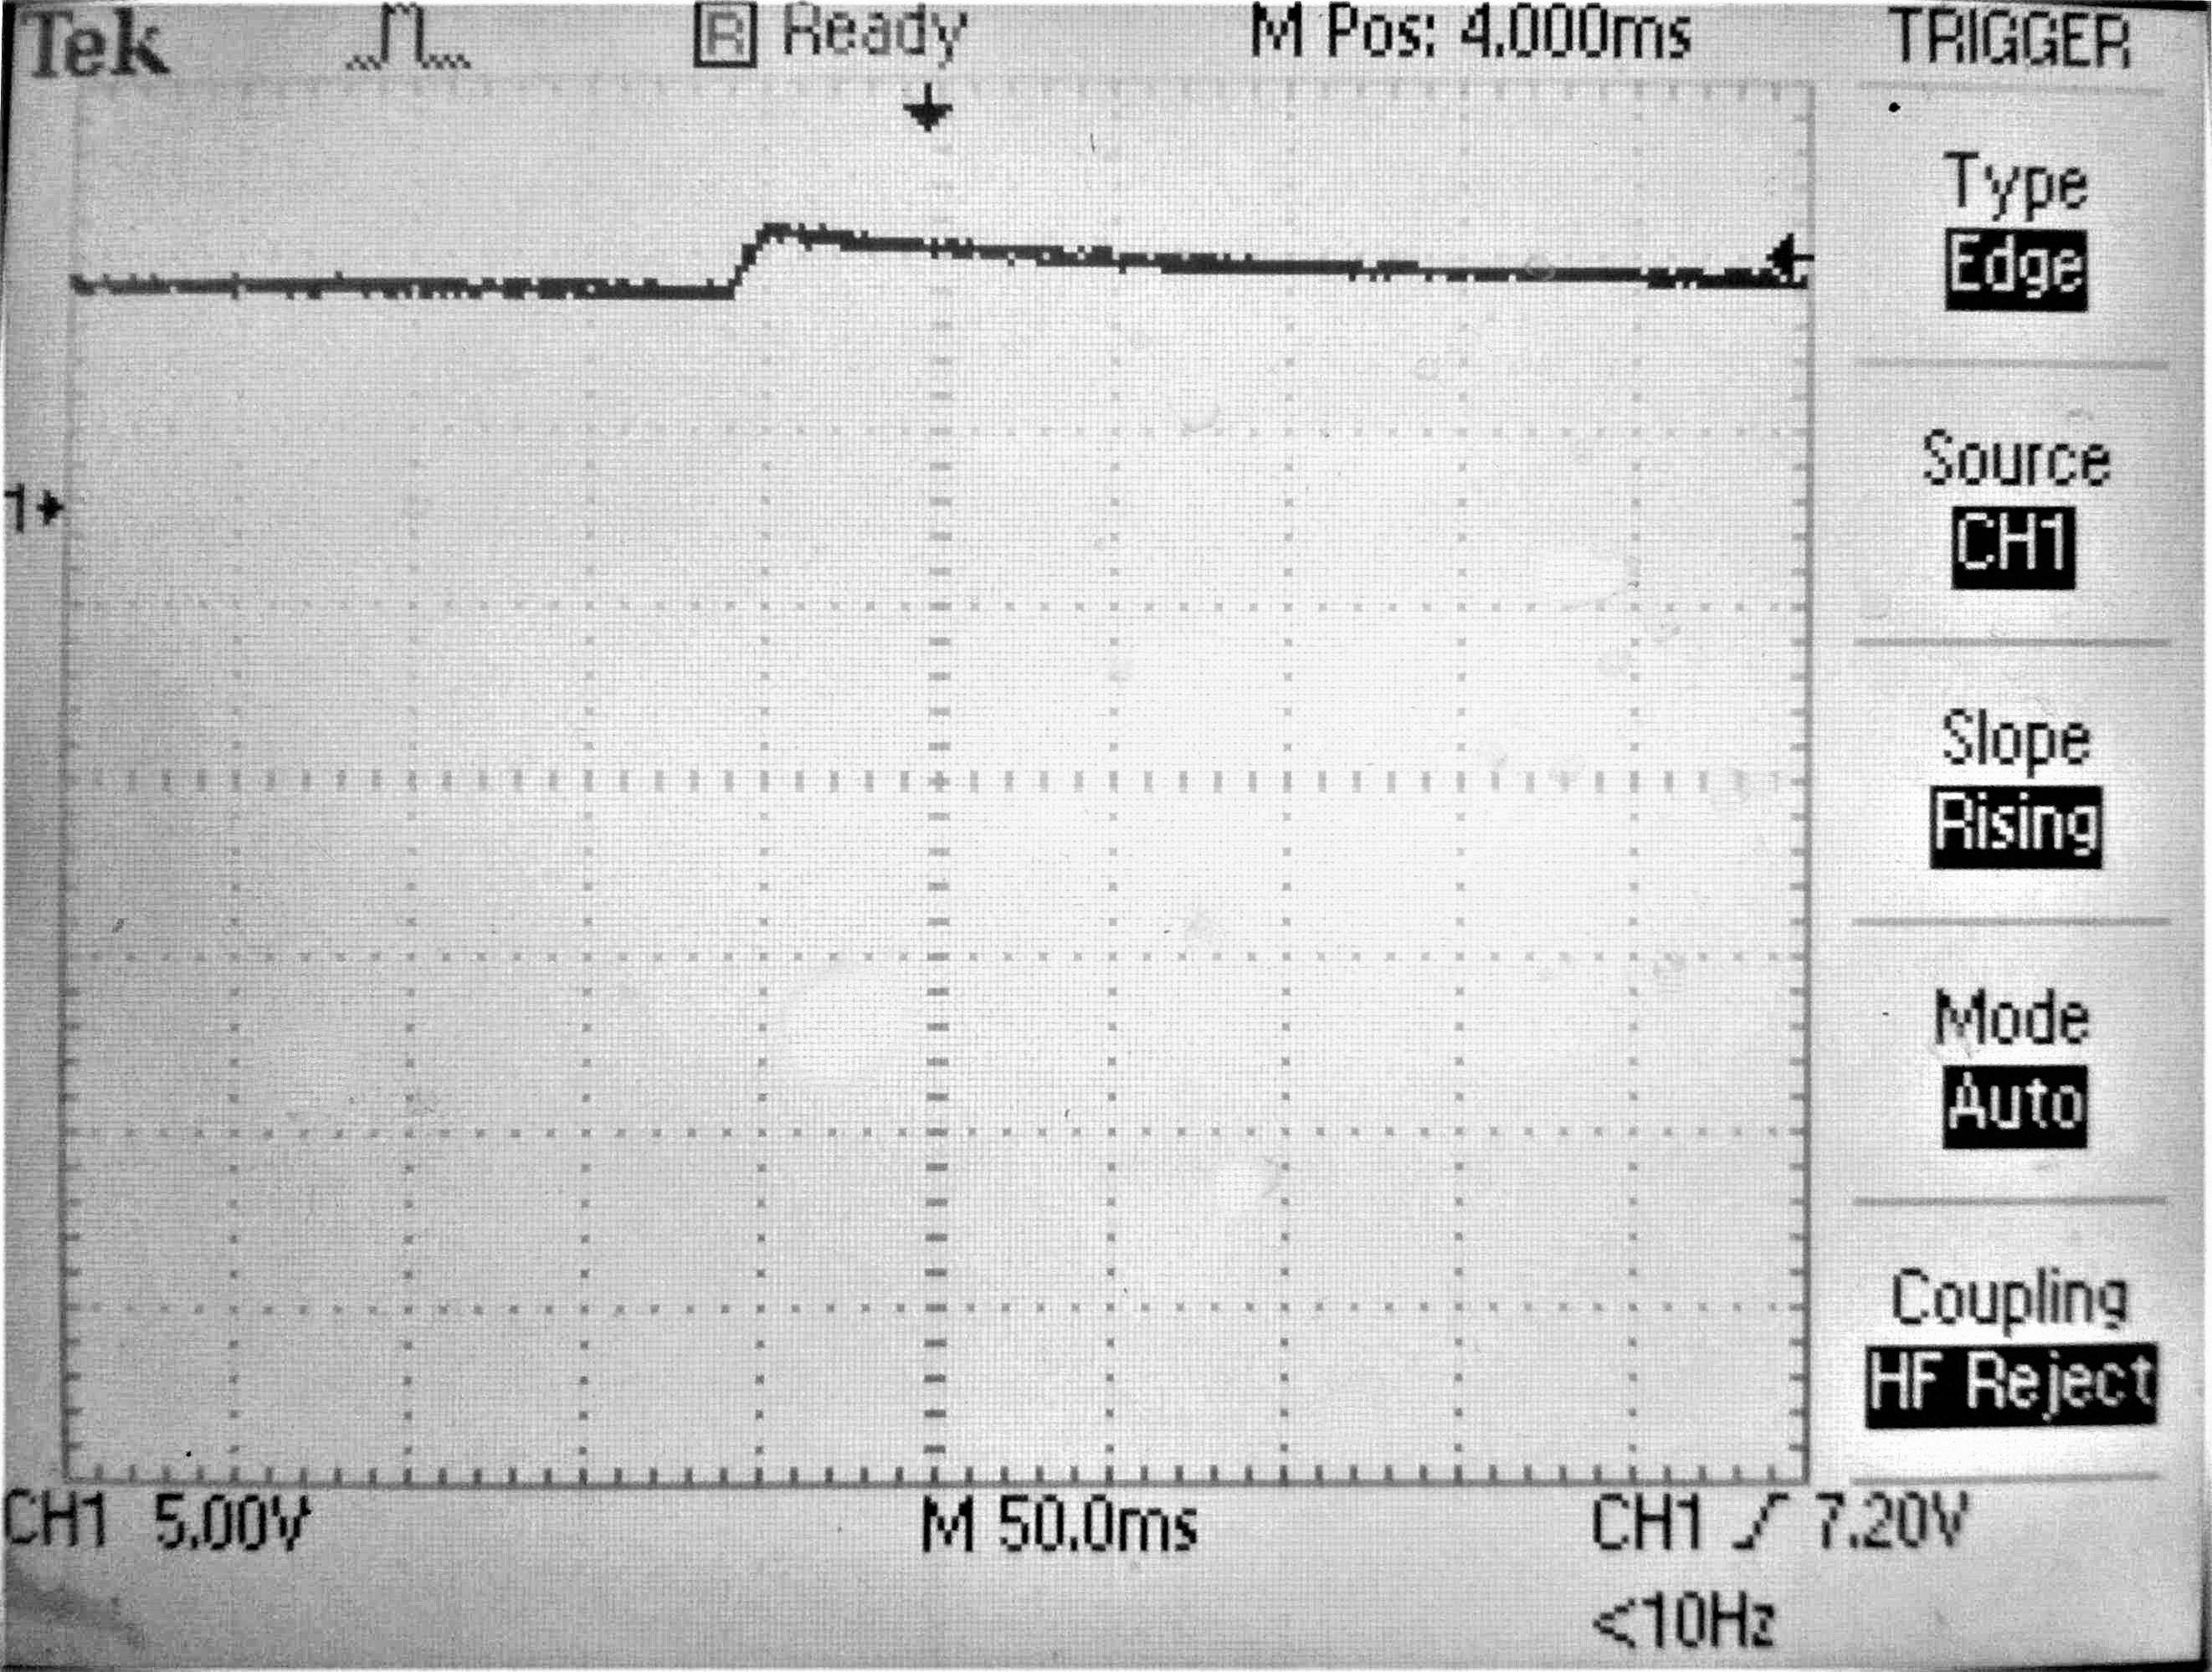
\includegraphics[width=0.45\textwidth]{rys03/zasilanieFiltr.jpg} \\
			\end{tabular}
			\caption{Napięcie zasilania a) przed filtracją b) po filtracji}
			\label{fig:filtracjaZasilania}
		\end{figure}
		Jak widać na rysunku \ref{fig:filtracjaZasilania} filtr znacznie ograniczył częstotliwość wahań napięcia. Jednak nie udało się ich wyeliminować całkowicie i pojawiają się okresowo. 
		
	\section{Zabezpieczenia tranzystorów}
	    W przypadku wykorzystywania elementów indukcyjnych m.in silników, należy zwrócić uwagę na ich zachowanie w przypadku zmian prądów w obwodzie. Następuje wtedy zjawisko samoindukcji i w cewce jest generowana siła elektromotoryczna. Zależność indukowanej siły elektromotorycznej od zmiany prądu przedstawia wzór \ref{eq:SEMcewki}.
	    \begin{equation}
	        E = -L \frac{di}{dt}
	        \label{eq:SEMcewki}
	    \end{equation}
	    gdzie: \\
	    E  – siła elektromotoryczna, \\
	    L – indukcyjność cewki, \\
        i – natężenie prądu płynącego przez cewkę, \\
        t – czas. \\
        Wynika z niego, że gwałtowne zmiany prądu występujące np. podczas sterowania sygnałem PWM powodują generowanie wysokich impulsów napięcia na cewce. Badania przeprowadzone na pompce wody potwierdzają rozważania teoretyczne. Przebieg napięcia podczas sterowania sygnałem PWM o wypełnieniu \SI{50}{\percent} został przedstawiony na rysunku \ref{fig:pompkaBezFiltracji}.
        \begin{figure}[ht]
			\centering
			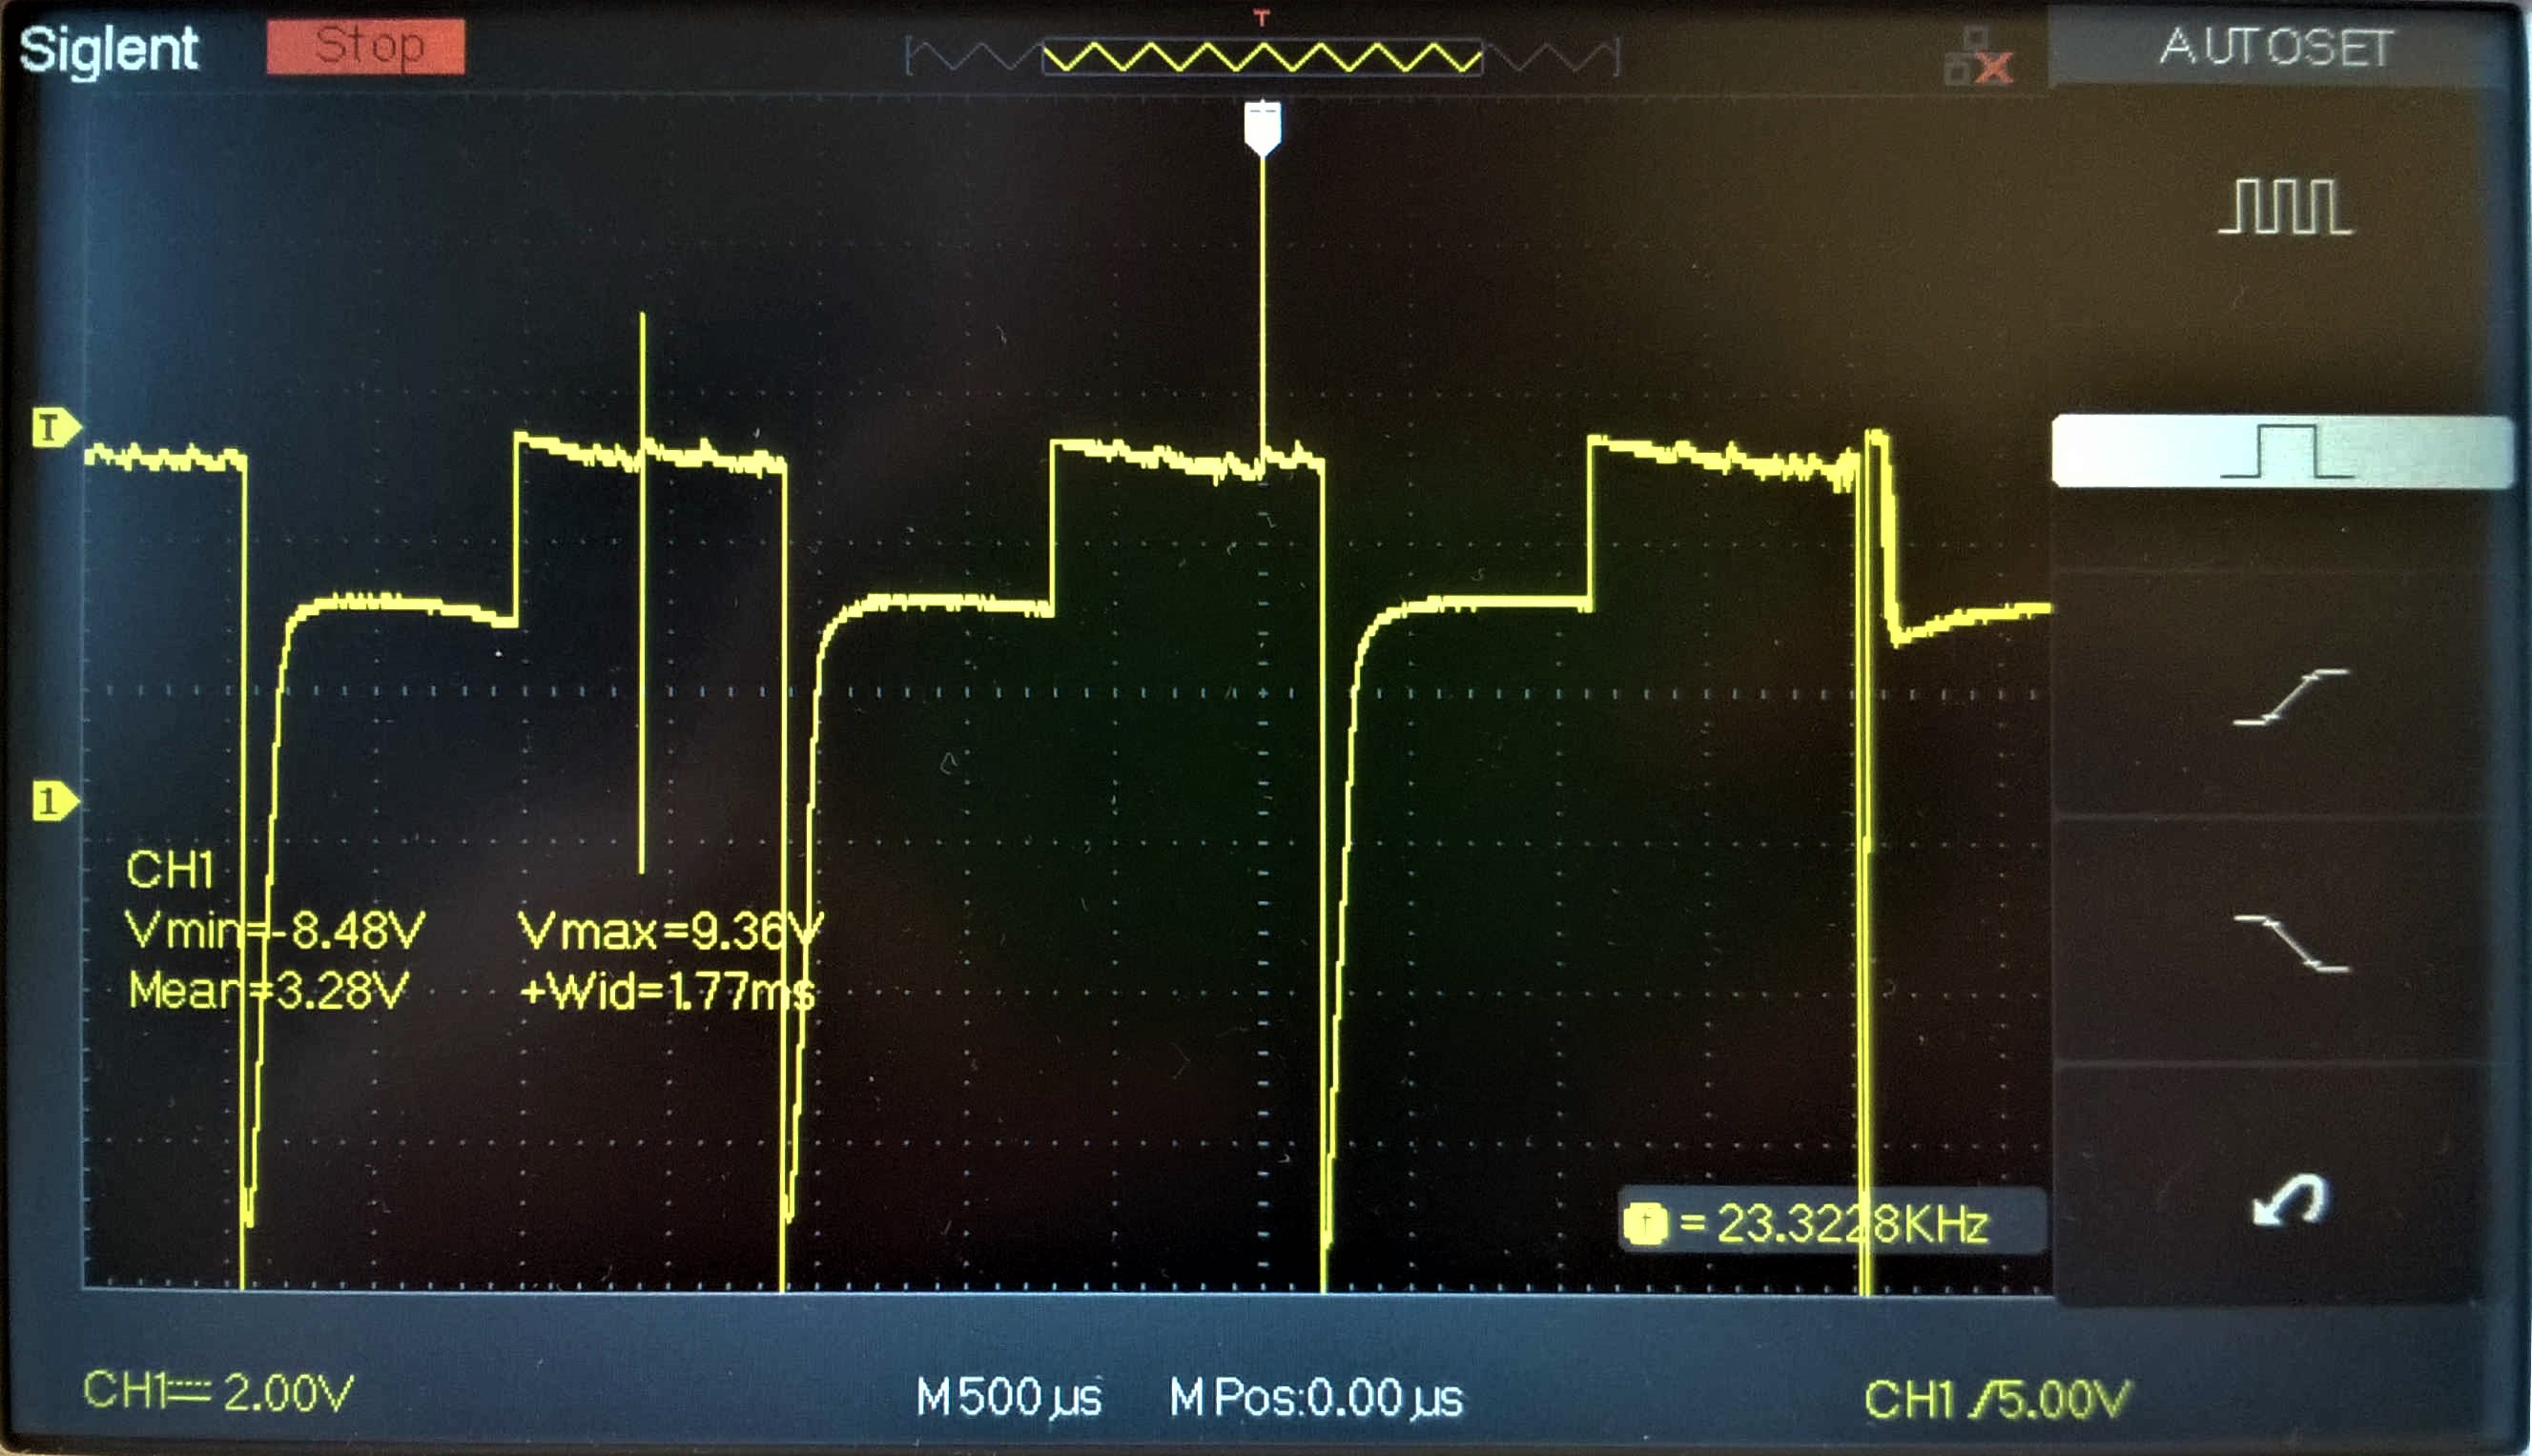
\includegraphics[width=0.45\textwidth]{rys03/przedSchottky.jpg}
			\caption{Napięcie na pompce wody bez filtracji}
			\label{fig:pompkaBezFiltracji}
		\end{figure}
		Widać na nim gwałtowne impulsy napięcia, znacznie przewyższające wartości sygnału PWM. Takie zachowanie może zniszczyć tranzystor sterujący. Dlatego aby zniwelować ten efekt stosuje się połączoną równolegle do zacisków elementu indukcyjnego diodę Schottkyego, dodatkowo można podłączyć także kondensator. Wyniki dla takich zabezpieczeń zostały przedstawione na rysunku \ref{fig:pompkaFiltracja}.
		\begin{figure}[ht]
			\centering
			\begin{tabular}{@{}ll@{}}
				a) & b) \\
				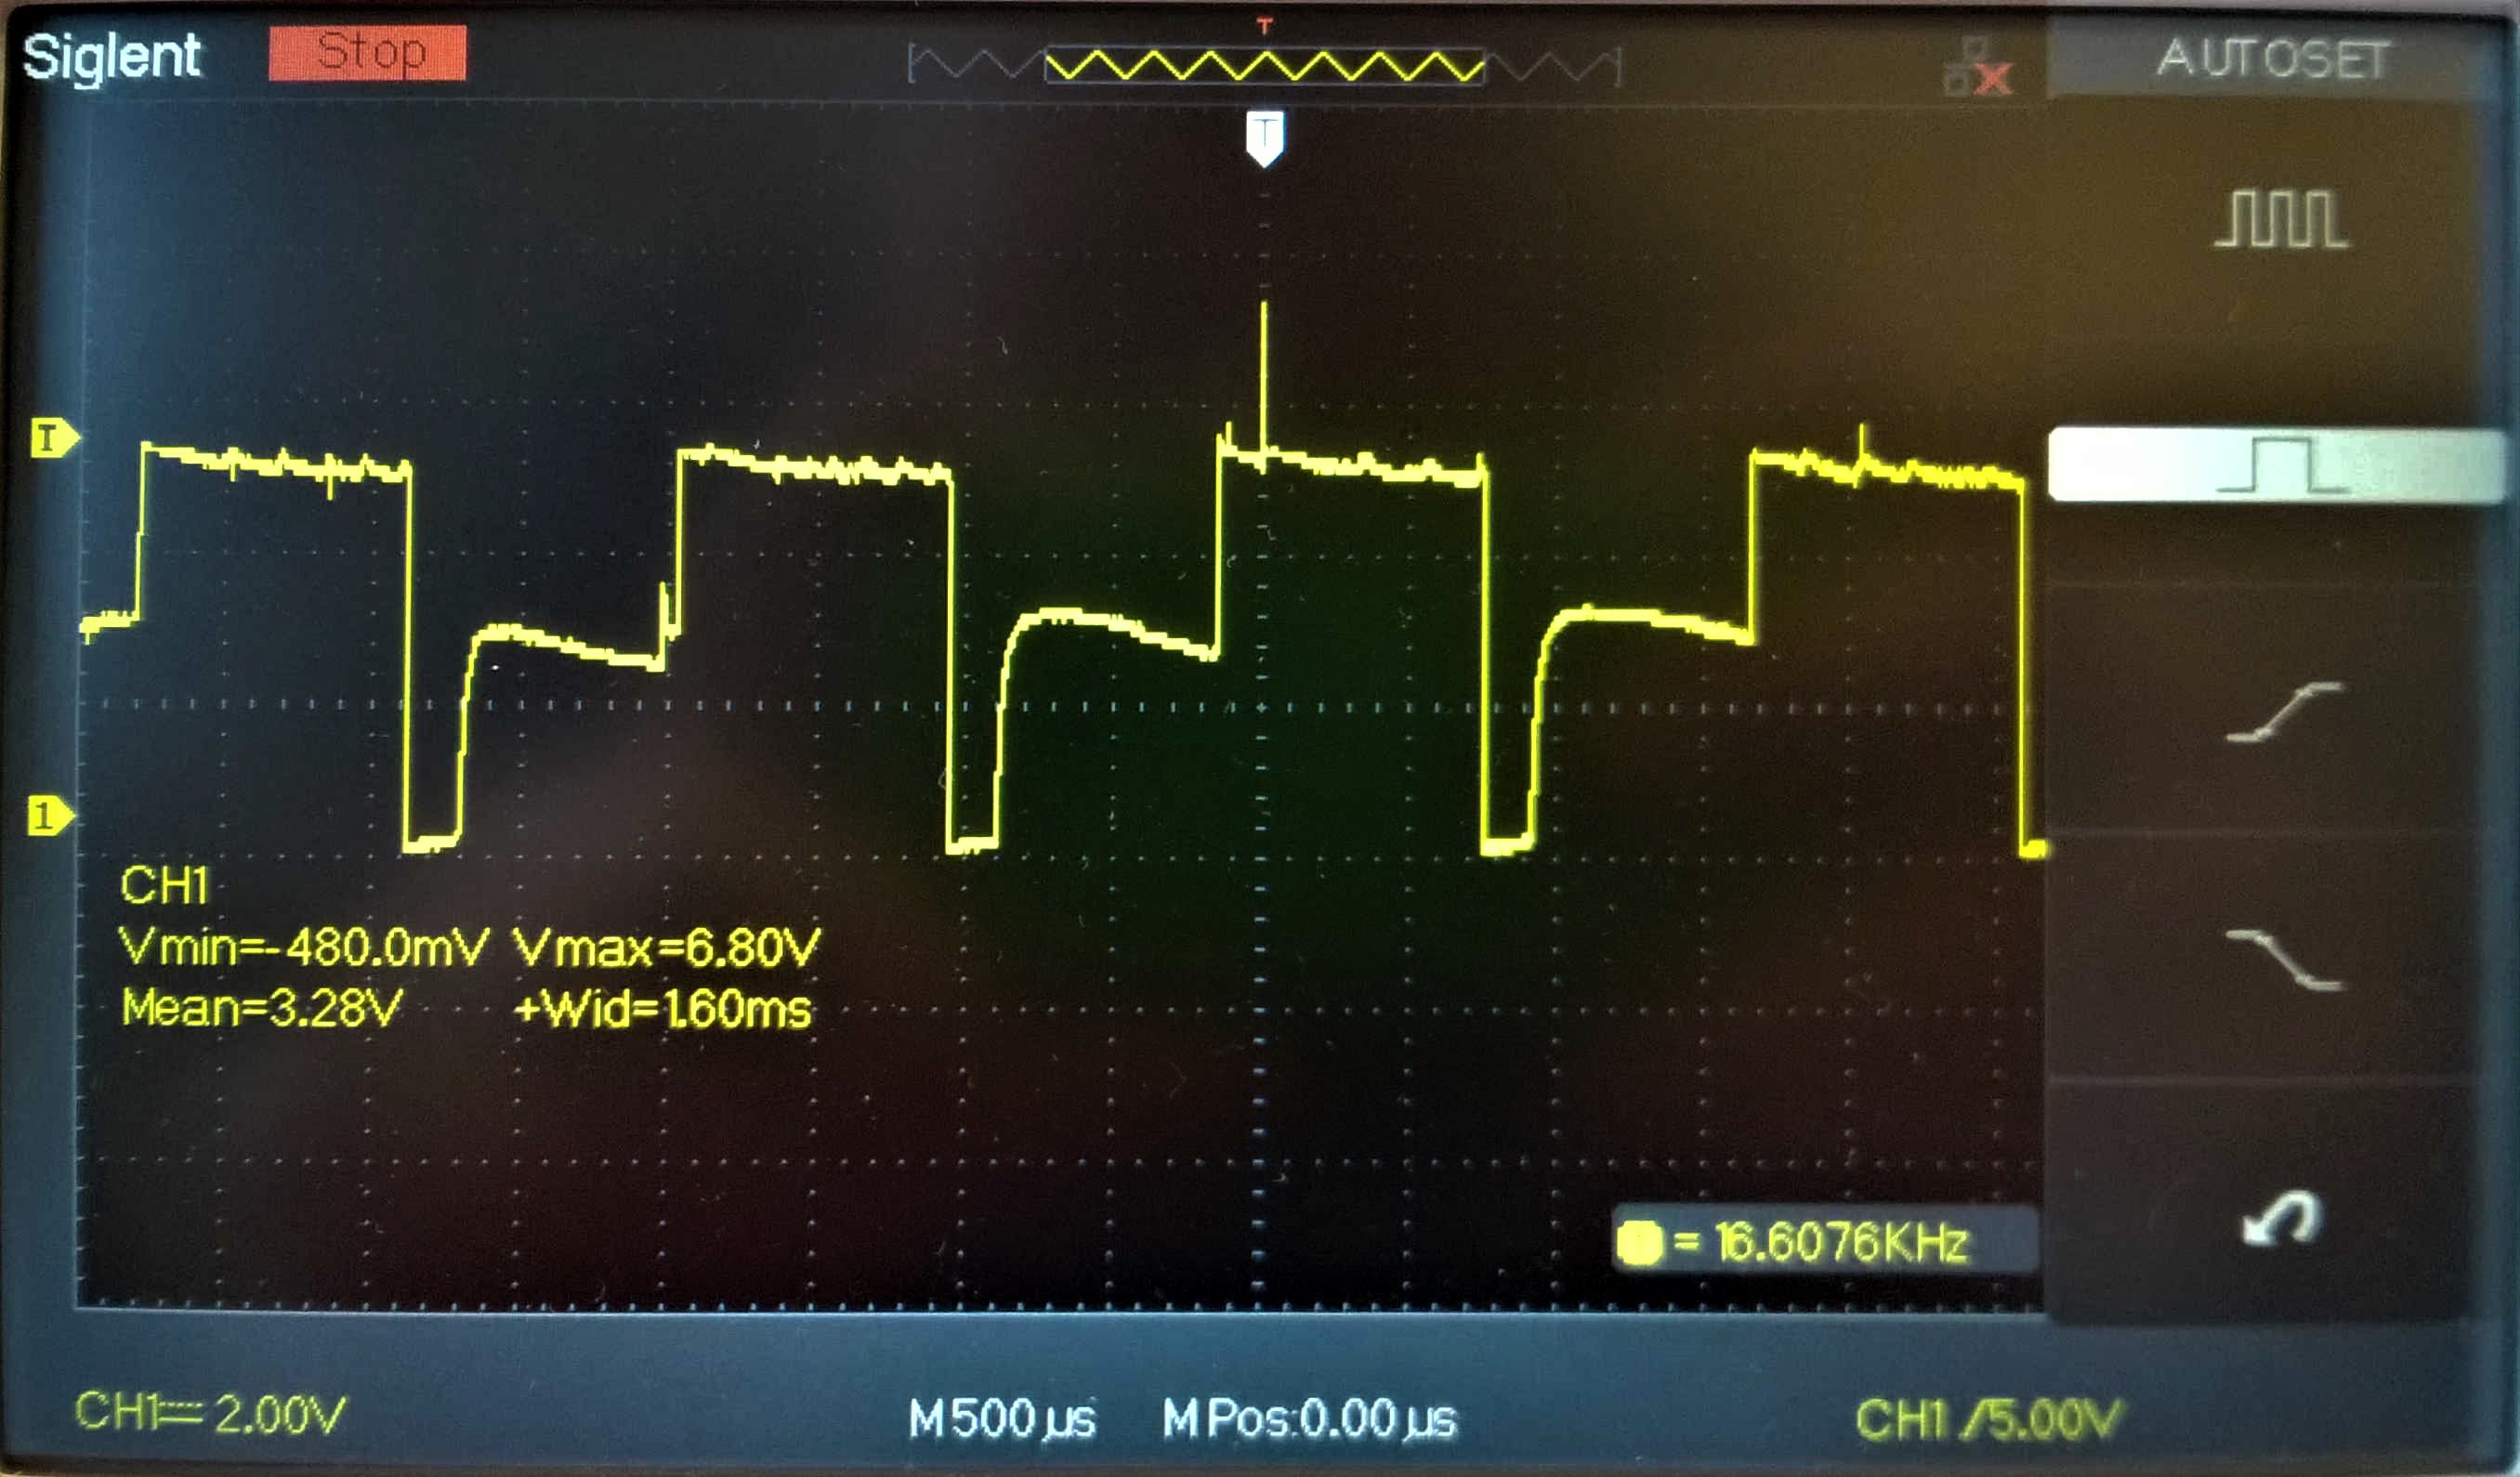
\includegraphics[width=0.45\textwidth]{rys03/schottky.jpg} & 
				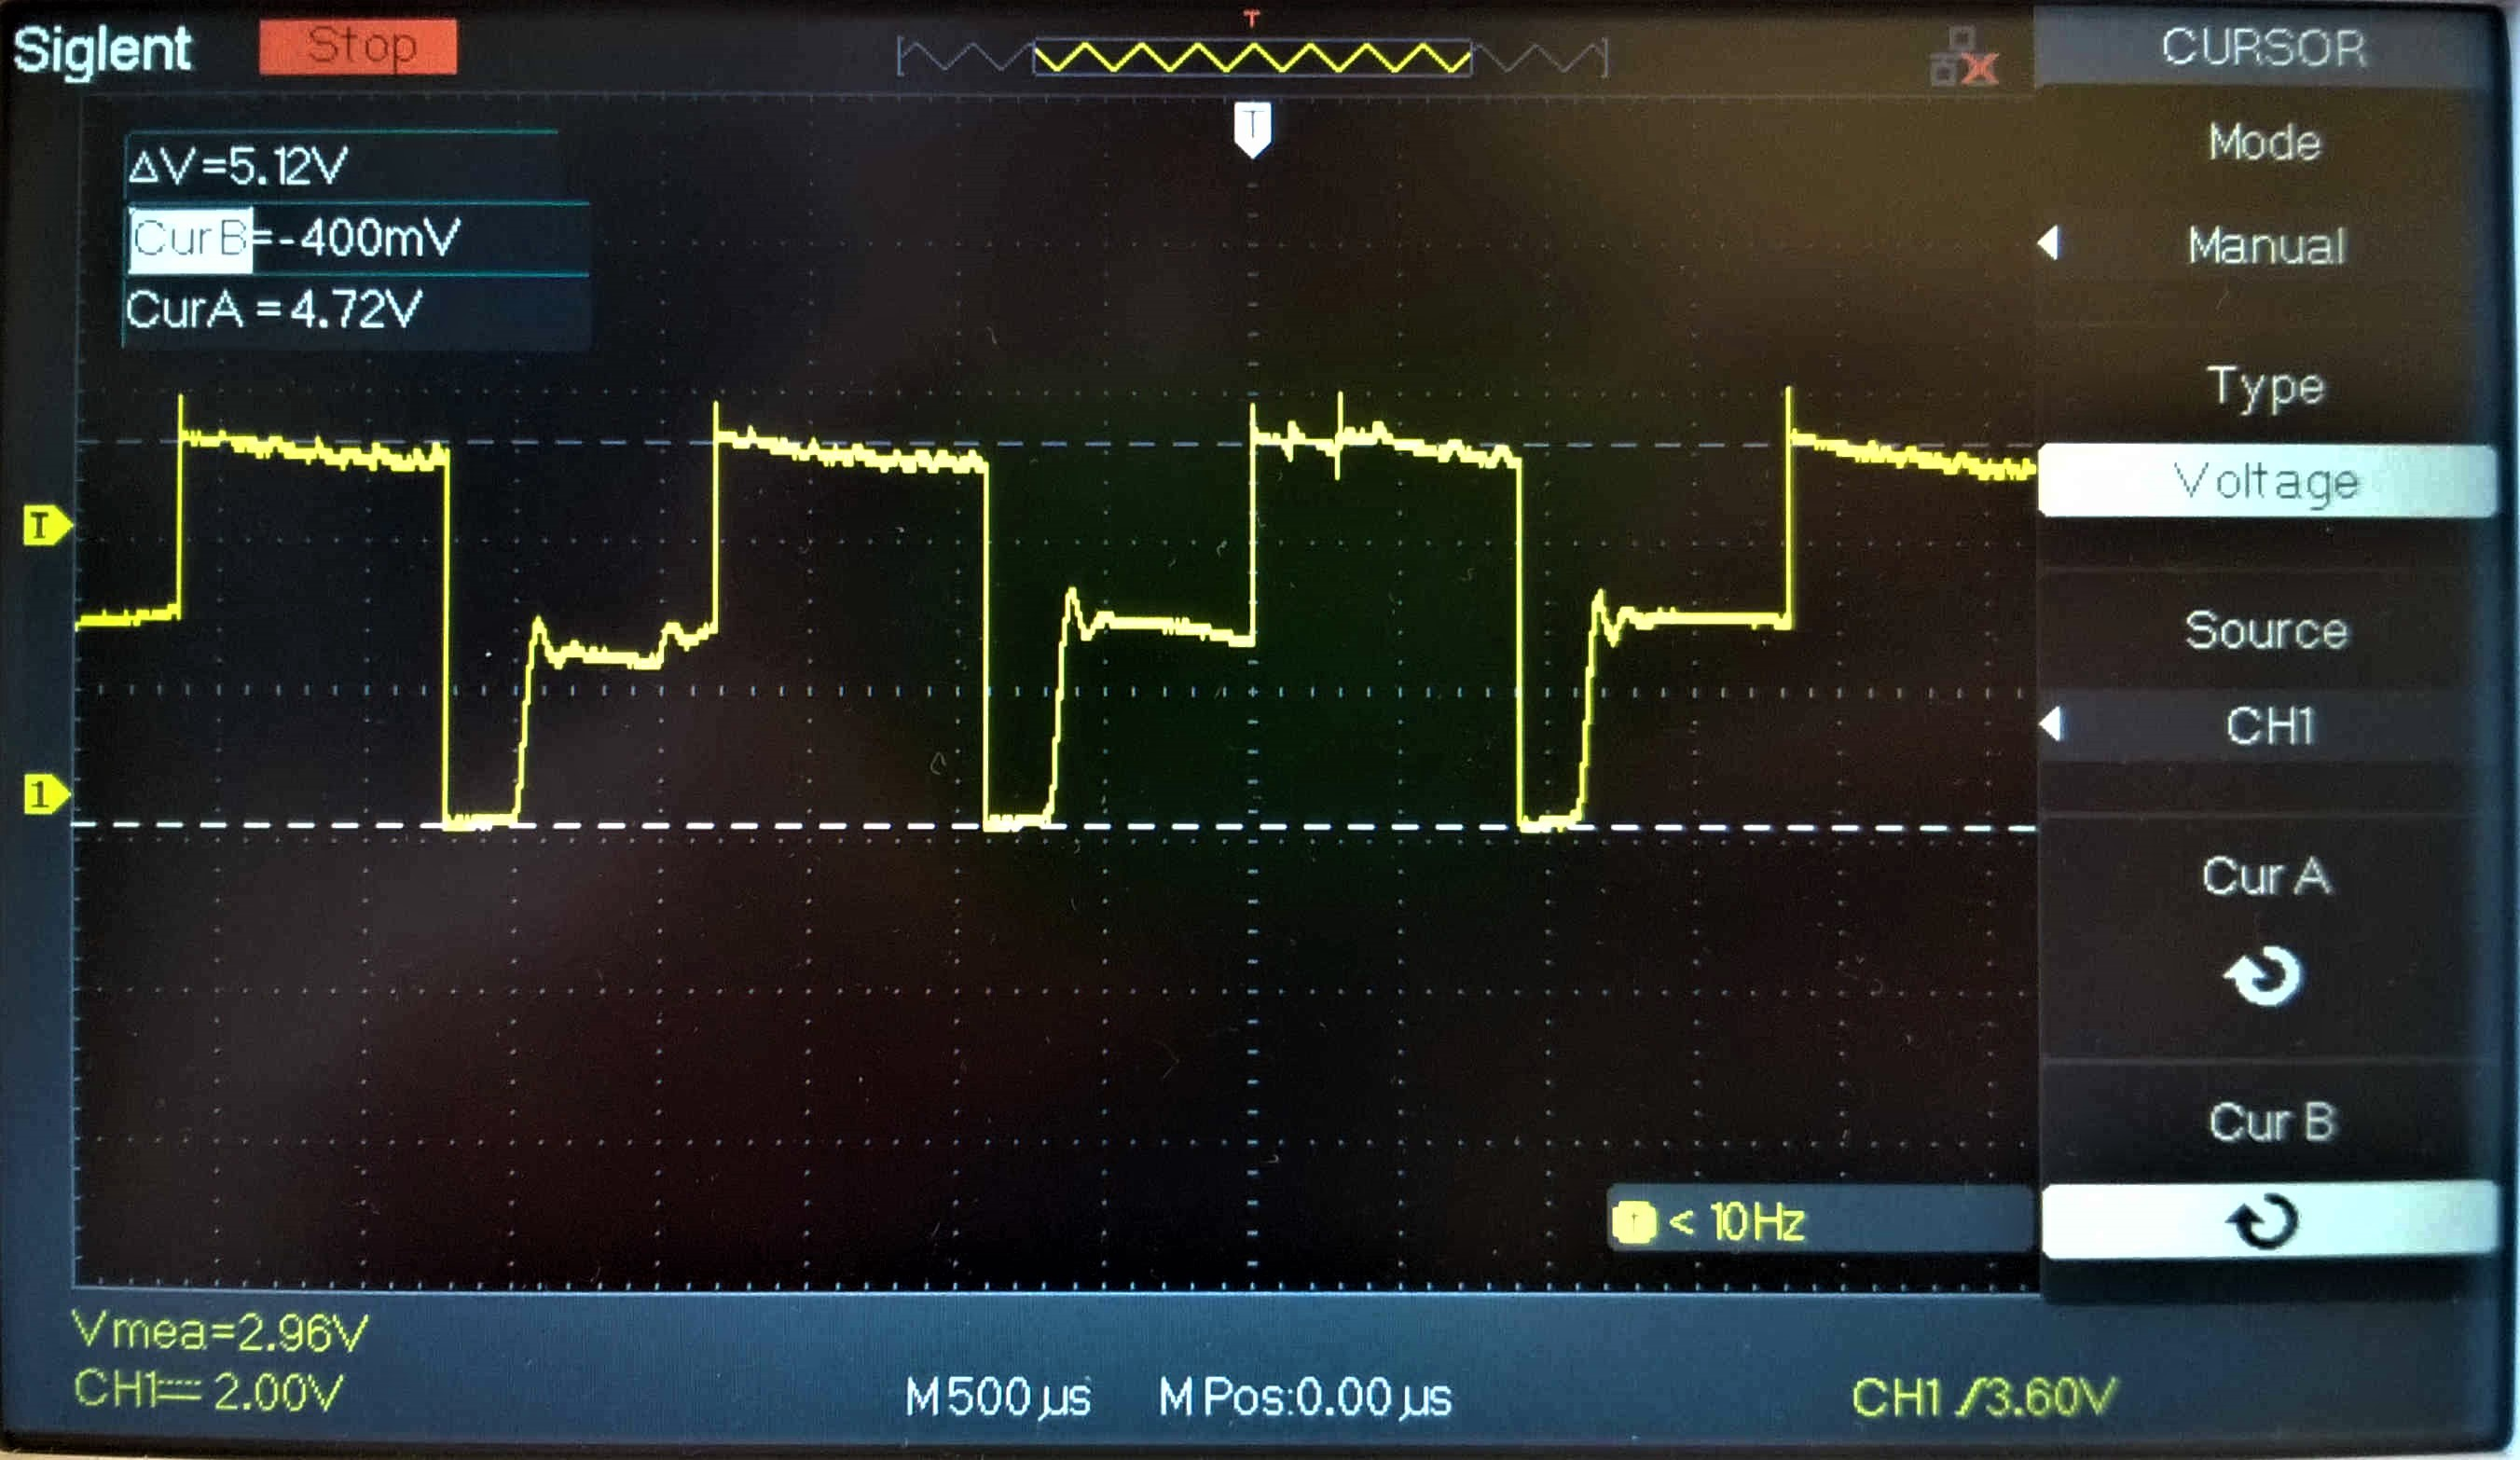
\includegraphics[width=0.45\textwidth]{rys03/schottkyZkondem.jpg} \\
			\end{tabular}
			\caption{Napięcie na pompce wody: a) z diodą Schottkyego b) z diodą Schottkyego i kondensatorem}
			\label{fig:pompkaFiltracja}
		\end{figure}
		Widać na nich ograniczenie przepięcia do wartości napięcia przewodzenia diody.
		
		W projekcie zastosowane zostały gotowe moduły sterowania silnikami, które rozwiązują przedstawiony problem.
\chapter{Redakcja pracy}
\section{Układ pracy}
Standardowo praca powinna być zredagowana w następującym układzie:

\noindent\fbox{\begin{minipage}{\dimexpr\textwidth-2\fboxsep-2\fboxrule\relax}
\begin{quote}
\item Strona tytułowa
\item Strona z dedykacją (opcjonalna)
\item Spis treści  
\item Spis rysunków (opcjonalny)
\item Spis tabel (opcjonalny)
\item Skróty (wykaz opcjonalny)
\item 1. Wstęp 
\begin{quote}
\item 1.1 Cel i zakres pracy 
\item 1.2 Układ pracy 
\end{quote}
\item 2. Kolejny rozdział
\begin{quote}
\item 2.1 Sekcja
\begin{quote}
\item 2.1.1 Podsekcja
\begin{quote}
\item Nienumerowana podpodsekcja
\begin{quote}
\item Paragraf
\end{quote}
\end{quote}
\end{quote}
\end{quote}
\item $\ldots$
\item \#. Podsumownie i wnioski
\item Literatura
\item A. Dodatek
\begin{quote}
\item A.1 Sekcja w dodatku
\end{quote}
\item $\ldots$
\item \$. Zawartość płyty CD/DVD
\item Indeks rzeczowy (opcjonalny)
\end{quote}
\end{minipage}}\\

Spis treści -- powinien być generowany automatycznie, z podaniem tytułów i numerów stron. Typ czcionki oraz wielkość liter spisu treści powinny być takie same jak w niniejszym wzorcu.

Spis rysunków, Spis tabel -- powinny być generowane automatycznie (podobnie jak Spis treści). Elementy te są opcjonalne (robienie osobnego spisu, w którym na przykład są tylko dwie pozycje specjalnie nie ma sensu).

Wstęp -- pierwszy rozdział, w którym powinien znaleźć się opis dziedziny, w jakiej osadzona jest praca, oraz wyjaśnienie motywacji do podjęcia tematu.  
W sekcji ,,Cel i zakres'' powinien znaleźć się opis celu oraz zadań do wykonania, zaś w sekcji ,,Układ pracy'' -- opis zawartości kolejnych rozdziałów.

Podsumowanie -- w rozdziale tym powinny być zamieszczone: podsumowanie uzyskanych efektów oraz wnioski końcowe wynikające z realizacji celu pracy dyplomowej.

Literatura -- wykaz źródeł wykorzystanych w pracy (do każdego źródła musi istnieć odpowiednie cytowanie w tekście). Wykaz ten powinien być generowany automatycznie.

Dodatki -- miejsce na zamieszczanie informacji dodatkowych, jak: Instrukcja wdrożeniowa, Instrukcja uruchomieniowa, Podręcznik użytkownika itp.
Osobny dodatek powinien być przeznaczony na opis zawartości dołączonej płyty CD/DVD. Założono, że będzie to zawsze ostatni dodatek.

Indeks rzeczowy -- miejsce na zamieszczenie kluczowych wyrazów, do których czytelnik będzie chciał sięgnąć. Indeks powinien być generowany automatycznie. Jego załączanie jest opcjonalne.
\section{Styl}
\label{sec:Styl}
Zasady pisania pracy (przy okazji można tu zaobserwować efekt wyrównania wpisów występujących na liście wyliczeniowej uzależnione od długości etykiety):
\begin{enumerate}[labelwidth=\widthof{\ref{last-item}},label=\arabic*.]
\item Praca dyplomowa powinna być napisana w  formie bezosobowej (,,w pracy pokazano ...''). Taki styl przyjęto na uczelniach w naszym kraju, choć w krajach anglosaskich preferuje się redagowanie treści w pierwszej osobie.
\item W tekście pracy można odwołać się do myśli autora, ale nie w pierwszej osobie, tylko poprzez wyrażenia typu: ,,autor wykazał, że ...''. 
\item Odwołując się do rysunków i tabel należy używać zwrotów typu: ,,na rysunku pokazano ...'', ,,w tabeli zamieszczono ...'' (tabela i rysunek to twory nieżywotne, więc ,,rysunek pokazuje'' jest niepoprawnym zwrotem).
\item Praca powinna być napisana językiem formalnym, bez wyrażeń żargonowych (,,sejwowanie'' i ,,downloadowanie''), nieformalnych czy zbyt ozdobnych (,,najznamienitszym przykładem tego niebywałego postępu ...'')
\item Pisząc pracę należy dbać o poprawność stylistyczną wypowiedzi
\begin{itemize}
\item trzeba pamiętać, do czego stosuje się ,,liczba'', a do czego ,,ilość'',
\item nie ,,szereg funkcji'' tylko ,,wiele funkcji'',
\item redagowane zdania nie powinny być zbyt długie (lepiej podzielić zdanie wielokrotnie złożone na pojedyncze zdania),
\item itp.
\end{itemize}
\item Zawartość rozdziałów powinna być dobrze wyważona. Nie wolno więc generować sekcji i podsekcji, które mają zbyt mało tekstu lub znacząco różnią się objętością. Zbyt krótkie podrozdziały można zaobserwować w przykładowym rozdziale~\ref{chap:podsumowanie}.
\item Niedopuszczalne jest pozostawienie w pracy błędów ortograficznych czy tzw.\ literówek -- można je przecież znaleźć i skorygować
automatycznie. \addtocounter{enumi}{9997} 
\item  Niedopuszczalne jest pozostawienie w pracy błędów ortograficznych czy tzw.\ literówek -- można je przecież znaleźć i skorygować
automatycznie. \label{last-item}
\end{enumerate}



\chapter{Uwagi techniczne}% 
\section{Rysunki}
W niniejszym szablonie numeracja rysunków odbywa się automatycznie według następujących reguł: rysunki powinny mieć numerację ciągłą w obrębie danego rozdziału, sam zaś numer powinien składać się z dwóch liczb rozdzielonych kropką. Pierwsza liczbą ma być numer rozdziału, drugą -- kolejny numer rysunku w rozdziale. Przykładowo: pierwszy rysunek w rozdziale 1 powinien mieć numer 1.1, drugi -- numer 1.2 itd., pierwszy rysunek w rozdziale 2 powinien mieć numer 2.1, drugi -- numer 1.2 itd. 

Rysunki powinny być wyśrodkowane na stronie wraz z podpisem umieszczonym na dole. Podpisy nie powinny kończyć się kropką. Czcionka podpisu powinna być mniejsza od czcionki tekstu wiodącego o 1 lub 2 pkt (w szablonie jest to czcionka rozmiaru \texttt{small}). Ponadto należy zachowywać odpowiedni odstęp między rysunkiem, podpisem rysunku a tekstem rozdziału. 
W~przypadku korzystania z szablon odstępy te regulowane są automatycznie. Podpis i grafika muszą stanowić jeden obiekt. Chodzi o to, że w edytorach tekstu typu Office podpis nie scala się z grafiką i czasem trafia na następną stronę, osieracając grafikę. Korzystającym z niniejszego szablonu i otoczenia \verb?\figure? takie osierocenie nigdy się nie zdarzy.  

Do każdego rysunku musi istnieć odwołanie w tekście (inaczej mówiąc: niedopuszczalne jest wstawienie do pracy rysunku bez opisu). Odwołania do rysunków powinny mieć postać: ,,Na rysunku~3.3 przedstawiono...'' lub ,,... co ujęto na odpowiednim schemacie (rys.~1.7)''. 
Jeśli odwołanie stanowi część zdania, to wtedy wyraz ,,rysunek'' powinien pojawić się w całości. Jeśli zaś odwołanie jest ujęte w nawias (jak w przykładzie), wtedy należy zastosować skrót ,,rys.''. Jeśli do stworzenia obrazka wykorzystano jakieś źródła, to powinny one być zacytowane w podpisie tegoż rysunku. 

Należy pamiętać o tym, że ,,rysunki'' to twory nieżywotne. W związku z tym nie mogą ''pokazywać''. Dlatego ,,rysunek~1.1 pokazuje ...'' jest stylistycznie niepoprawne. Zamiast tego zwrotu trzeba użyć ,, na rysunku~1.1 pokazano ...''.

Rysunki można wstawiać do pracy używając polecenia \verb|\includegraphics|. Zalecane jest, aby pliki z grafikami były umieszczane w katalogach 
odpowiadających numerom rozdziałów czy literom dodatków: \verb|rys01|, \verb|rysA| itd. Sposób wstawiania rysunków do pracy zademonstrowano na przykładze rysunków~\ref{fig:kanji-giri} i \ref{fig:alfabeta}.

\begin{lstlisting}[label=list:includegraphics,caption=Kod źródłowy przykładów wstawiania rysunków do pracy,basicstyle=\footnotesize\ttfamily]
\begin{figure}[ht]
 \centering
  
\includegraphics[width=0.3\linewidth]{rys05/kanji-giri}
 \caption{Dwa znaki kanji - giri}
 \label{fig:kanji-giri}
\end{figure}

\begin{figure}[htb]
 \centering
  \begin{tabular}{@{}ll@{}}
  a) & b) \\
  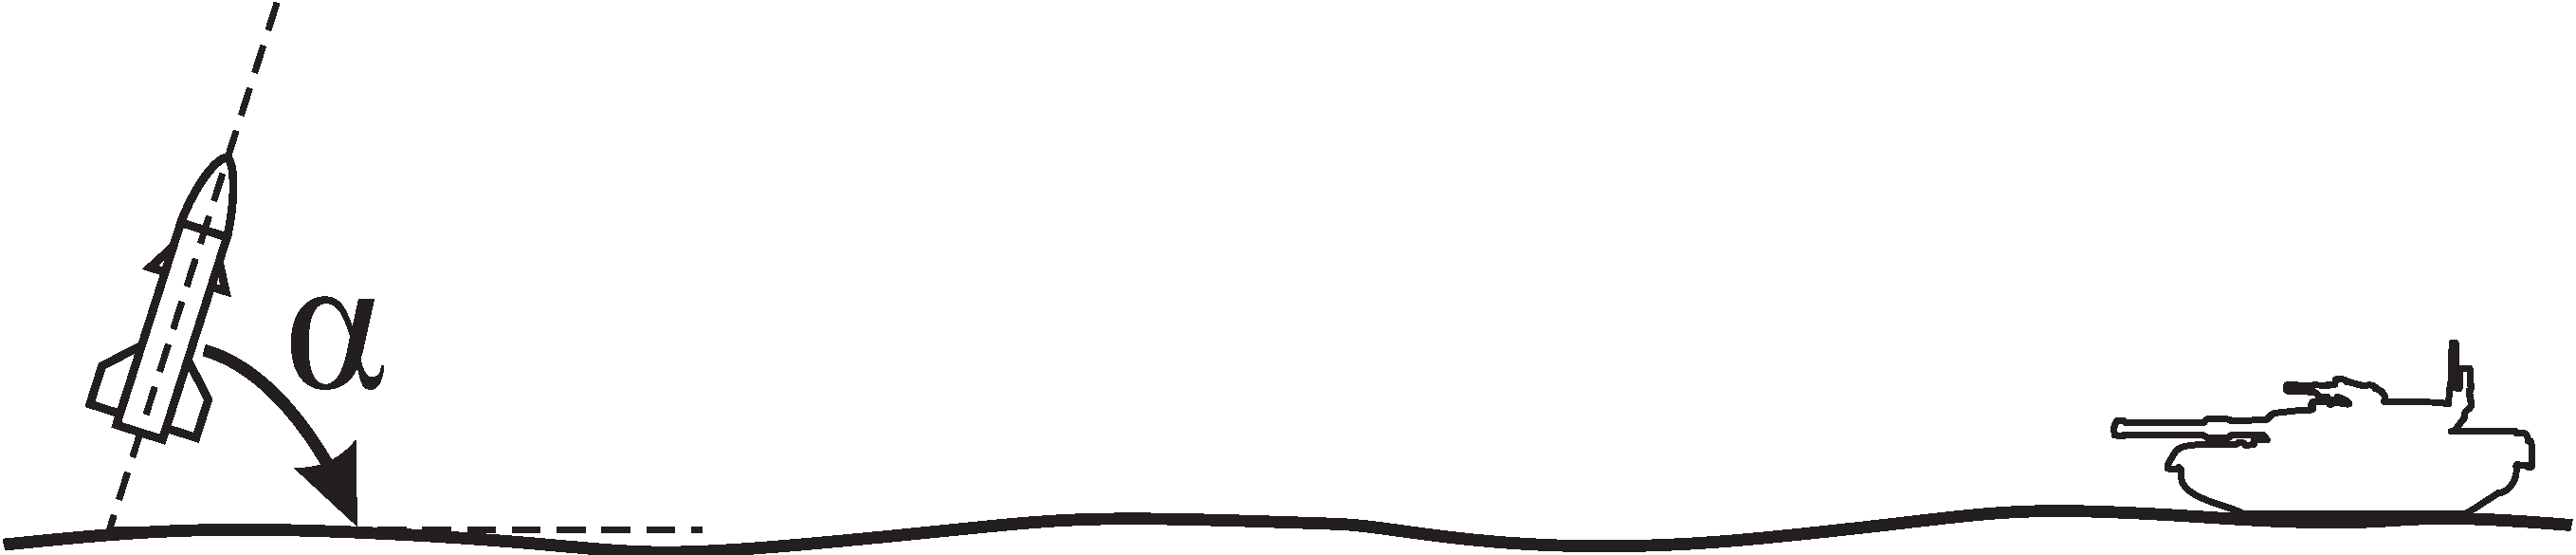
\includegraphics[width=0.475\textwidth]{rys05/alfa1} & 
  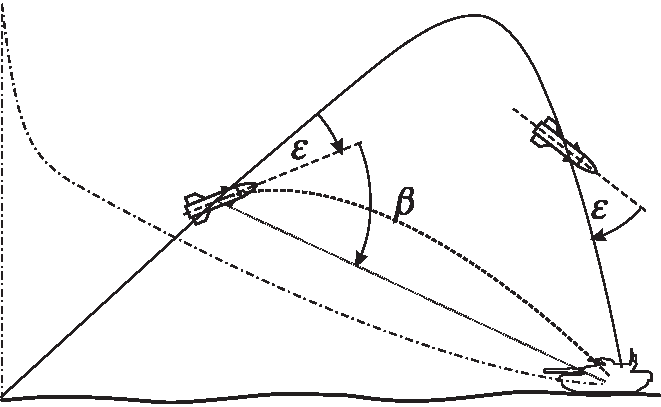
\includegraphics[width=0.475\textwidth]{rys05/beta1}
  \end{tabular}
 \caption{Wyznaczanie trajektorii lotu rakiety: 
 a) trzy podejścia, b) podejście praktyczne}
 \label{fig:alfabeta}
\end{figure}
\end{lstlisting}

\begin{figure}[ht]
	\centering
		\includegraphics[width=0.3\linewidth]{rys05/kanji-giri}
	\caption{Dwa znaki kanji -- giri}
	\label{fig:kanji-giri}
\end{figure}

\begin{figure}[htb]
  \centering
	\begin{tabular}{@{}ll@{}}
	a) & b) \\
  \includegraphics[width=0.475\textwidth]{rys05/beta1} & 
	\includegraphics[width=0.475\textwidth]{rys05/alfa1}
	\end{tabular}
  \caption{Wyznaczanie trajektorii lotu rakiety: a) trzy podejścia, b) podejście praktyczne}
  \label{fig:alfabeta}
\end{figure}

Grafiki wektorowe powinny być dostarczone w plikach o formacie pdf. Rozmiar strony w~pliku pdf powinien być troszeczkę większy niż zamieszczona na nim grafika (proszę spojrzeć na przykłady grafik wykorzystanych w niniejszym szablonie). Chodzi o to, aby na rysunku nie pojawiała się niepotrzebna biała przestrzeń. Grafiki rastrowe (głównie zrzuty z ekranu bądź zdjęcia) powinny być dostarczane w plikach o formacie png z~kompresją bezstratną. Zastosowanie kompresji stratnej, jak jpg, wprowadza niepotrzebne artefakty. Podobnie jak w przypadku grafik wektorowych, grafiki rastrowe nie powinny mieć białych marginesów.

Na rysunkach nie powinno stosować się 100\% czarnego wypełnienia, bo robią się plamy przebijające się przez kartkę. Zamiast tego wypełnienie powinno być ok.\ 90\% czerni.

Czcionka na rysunkach nie może być większa od czcionki wiodącej tekstu (jedyny wyjątek to np.\ jakieś nagłówki).
Należy stosować czcionkę kroju Arial, Helvetica bądź tego samego kroju co czcionka dokumentu (\texttt{texgyre-termes}). 

Jeśli na jednym rysunku pojawić się ma kilka grafik, to zamiast stosować \texttt{subfigure} lub inne otoczenia należy wstawić grafiki w tabelę, opisać ją indeksami a) i b), a potem odnieść się do tego w podpisie (rys.~\ref{fig:alfabeta}).
Czasem pomaga w pozycjonowaniu rysunków użycie komendy:
\verb+\vtop{\vskip3ex\hbox{\includegraphics[width=0.475\textwidth]{nazwa}}}+

Na rysunkach nie wolno nadużywać kolorów oraz ozdobników (wiele narzędzi do tworzenia diagramów dostarcza grafikę z cieniowaniem, gradacją kolorów itp.\  co niekoniecznie przekłada się na czytelność rysunku).

Podczas rozbienia zrzutów z ekranu należy zadbać o to, by taki zrzut był czytelny po wydrukowaniu. Czyli aby pojawiające się literki były wystarczająco duże, a przestrzenie bez treści -- relatywnie małe.
Przystępując do robienia zrzutu trzeba odpowiednio wyskalować elementy na ekranie. Na przykład robiąc zrzut z przeglądarki FF najpierw należy wcisnąć CTR--0 (domyślne skalowanie), potem CTR--{}- (zmniejszenie skali o stopień). Potem dobrze jest zawęzić okno przeglądarki tak, by interesująca treść wypełniła je w całości. Jeśli na obserwowanej stronie jest zbyt dużo pustych obszarów, to należy je jakoś zawęzić (sterując wielkością okna przeglądarki lub aktywnymi elementami interfejsu użytkownika). Zrzut bowiem wcale nie musi być odzwierciedleniem 1:1 domyślnego układu obserwowanych elementów. Ważne jest, by na zrzucie z ekranu pokazać interesujący, opisywany fragment i żeby ten fragment był czytelny.
	
Czasem problemem jest tworzenie zrzutów z ekranu, gdy występują na nim dane wrażliwe. Istnieją dwa sposoby na radzenie sobie z tym problemem.
Pierwszy polega na zastąpieniu w~systemie danych danych rzeczywistych danymi testowymi -- wygenerowanymi tylko do celów prezentacji.
Zrzut robi się wtedy na bazie danych testowych.
Drugi polega na wykonaniu zrzutu z~ekranu, na którym pokazano dane rzeczywiste, i następnie zamianie tych danych już w pliku graficznym
za pomocą odpowiedniego edytora (np.~\texttt{gimp}). Czyli oryginalny zrzut z ekranu należy otworzyć w edytorze, a potem
nadpisać oryginalny tekst własnym tekstem. Konieczne jest wtedy dobranie odpowiednich czcionek aby nie było widać
wprowadzonych zmian. 
\begin{quotation}
Uwaga: takie manipulowanie zrzutami jest usprawiedliwione jedynie w przypadku konieczności ochrony danych wrażliwych czy też lepszego pokazania wybranych elementów. Nie może to prowadzić generowania fałszywych rezultatów!!!
\end{quotation}

\section{Wstawianie kodu źródłowego}
Kod źródłowy można wstawiać jako blok tekstu pisany czcionką maszynową. Używa się do tego otoczenie \verb?\lstlisting?. W atrybutach otoczenia można zdefiniować tekst podpisu wstawianego wraz z numerem nad blokiem, etykietę do tworzenia odwołań, sposób formatowania i~inne ustawienia. Zaleca się stosowanie w tym otoczeniu następujących parametrów:
\begin{lstlisting}[basicstyle=\footnotesize\ttfamily]
\begin{lstlisting}[label=list:req1,caption=Initial HTTP Request,
                   basicstyle=\footnotesize\ttfamily]
\end{lstlisting}
Szczególnie przydatne podczas wstawiania większej ilości kodu źródłowego jest zastosowanie parametru \verb+basicstyle=\footnotesize\ttfamily+. Dzięki niemu zmniejsza się czcionka, a~przez to na stronie można zmieścić dłuższe linijki kodu. Użycie tak zdefiniowanego parametru nie jest jednak sztywnym zaleceniem. Wielkość czcionki można dobierać do potrzeb. 
{\belowcaptionskip=-10pt
\begin{lstlisting}[label=list:req1,caption=Initial HTTP Request,
                   basicstyle=\footnotesize\ttfamily]
GET /script/Articles/Latest.aspx HTTP/1.1
Host: www.codeproject.com
Connection: keep-alive
Cache-Control: max-age=0
Accept: text/html,application/xhtml+xml,application/xml
User-Agent: Mozilla/5.0 ...
Accept-Encoding: gzip,deflate,sdch
Accept-Language: en-US...
Accept-Charset: windows-1251,utf-8...
\end{lstlisting}
}
Można też sformatować kod bez stosowania numerowanego podpisu (wtedy nie zamieszcza się \texttt{caption} na liście atrybutów).
\begin{lstlisting}[basicstyle=\footnotesize\ttfamily]
GET /script/Articles/Latest.aspx HTTP/1.1
Host: www.codeproject.com
Connection: keep-alive
Cache-Control: max-age=0
Accept: text/html,application/xhtml+xml,application/xml
User-Agent: Mozilla/5.0 ...
Accept-Encoding: gzip,deflate,sdch
Accept-Language: en-US...
Accept-Charset: windows-1251,utf-8...
\end{lstlisting}

Istnieje możliwość wstawiania kodu źródłowego w bieżącej linijce tekstu. Można to zrobić na kilka sposobów:
\begin{itemize} 
\item korzystając z polecenia \verb?\texttt? ustawiającego czcionkę maszynową, jak w przykładzie \texttt{tutaj} (efekt zastosowania komendy \verb?\texttt{tutaj}?). Problemem jednak mogą okazać się znaki podkreślenia i inne znaki kontrolne.
\item korzystają z otoczenia \verb?\verb? zapewniającego wypisanie kodu czcionką maszynową jak w~przykładzie \verb|tutaj| (efekt zastosowania komendy \verb?\verb|tutaj|?). Problemem jest to, że polecenie \verb?\verb? nie potrafi łamać dłuższego tekstu.
\item korzystając z polecenia \verb?\lstin? umożliwiającego wypisanie kodu czcionką ustawianą w~opcjach jak w przykładzie
\lstset{basicstyle=\ttfamily}\lstinline{tutaj} (efekt komendy \verb+\lstset{basicstyle=\ttfamily}\lstinline{tutaj}+) lub \lstinline[basicstyle=\ttfamily]=tutaj= (efekt komendy \verb+\lstinline[basicstyle=\ttfamily]=tutaj=+).
\end{itemize}

\section{Wykaz literatury oraz cytowania}
\label{sec:literatura}
Cytowania powinny być zamieszczane w tekście z użyciem komendy \verb+\cite{}+. Jej argumentem powinien być klucz cytowanej pozycji (lub lista kluczy  rozdzielonych przecinkiem bez spacji, jeśli takich pozycji w danym miejscu cytuje się więcej) jaki jest używany w bazie danych bibliograficznych (plik \texttt{dokumentacja.bib}). Po kompilacji \texttt{bibtex} i \texttt{pdflatex} w tekście pojawia się właściwy odsyłacz do pozycji w wykazie literatury (ujęty w kwadratowe nawiasy -- zgodnie z~tym, co definiuje styl \texttt{plabbrv.bst}), zaś w samym wykazie (rozdział Literatura) -- zacytowana pozycja. Przykładem cytowania jest: ,,dobrze to opisano w pracach~\cite{JS07,SQL2}'' (gdzie zastosowano komendę \verb?\cite{JS07,SQL2}?).

Co do zawartości rekordów bibliograficznych - style bibtexowe potrafią ,,skracać'' imiona (czyli wstawiać, jeśli taka wola, inicjały zamiast pełnych imion). Niemniej dobrze jest od razu przyjąć jakąś konwencję. Proponuje się, aby w rekordach od razu wstawiane były inicjały zamiast pełnych imion.

Niekiedy tytuły prac zawierają wyrazy z dużymi i małymi literami. Takie tytuły należy brać w podwójne nawiasy klamrowe, aby \texttt{bibtex} nie zamienił ich na postać, w której poza pierwszą literą pozostałe są małe.

Jeśli jakiś cytowany zasób pochodzi z Internetu, to jego rekord w pliku \texttt{bib} powinien wyglądać jak niżej.
\begin{lstlisting}[basicstyle=\footnotesize\ttfamily]
@INPROCEEDINGS{SQL2, 
  title={{A MySQL-based data archiver: preliminary results}}, 
  author={Bickley, M. and Slominski, Ch.},
  booktitle = {{Proceedings of ICALEPCS07}},
	month = oct,
	day = {15--19},
	year={2007}, 
  note={\url{http://www.osti.gov/scitech/servlets/purl/922267} 
	[dostęp dnia 20 czerwca 2015]}
}
\end{lstlisting}
A to inny przykład rekordu danych bibliograficznych:
\begin{lstlisting}[basicstyle=\footnotesize\ttfamily]
@TechReport{JS07,
	author = {Jędrzejczyk, J. and Śródka, B.},
	title  ={Segmentacja obrazów metodą drzew decyzyjnych},
	year = {2007},
	institution = {Politechnika Wrocławska, Wydział Elektroniki}
}
\end{lstlisting}

\section{Indeks rzeczowy}
\label{sec:indeks}
Generowanie indeksu \index{generowanie!-- indeksu} po trosze wygląda jak generowanie wykazu literatury \index{generowanie!-- wykazu literatury}-- wymaga kilku kroków. Podczas pierwszej kompilacji \texttt{pdflatex} generowany jest plik z rozszerzeniem \texttt{*.idx} (zawierający ,,surowy indeks''). Następnie, bazując na tym pliku, generowany jest plik z rozszerzeniem \texttt{*.ind} zawierający sformatowane dane. Ten krok wymaga uruchomienia odpowiedniego narzędzia oraz zastosowania plik z definicją stylu \texttt{Dyplom.ist}. W kroku ostatnim dokonuje się kolejnej kompilacji \texttt{pdflatex} (dzięki niej w wynikowym dokumencie pojawi się Indeks rzeczowy). Domyślnie Indeks rzeczowy zostanie sformatowany w~układzie dwukolumnowym.

Oczywiście aby to wszystko zadziałało w kodzie szablonu należy umieścić odpowiednie komendy definiujące elementy indeksu rzeczowego (\verb?\index?) oraz wstawiające sformatowany Indeks rzeczowy do dokumentu wynikowego (\verb?\printindex?). Więcej informacji o tworzeniu indeksu rzeczowego można znaleźć na stronie \url{https://en.wikibooks.org/wiki/LaTeX/Indexing}. Poniżej przedstawiono przykłady komend użytych w szablonie do zdefiniowania elementów indeksu rzeczowego:
\begin{itemize}
\item \verb?\index{linia komend}? -- pozycji główna.
\item \verb?\index{generowanie!-- indeksu}? -- podpozycja.
\end{itemize}

Generowanie pliku \texttt{*.ind} można inicjować na kilka sposobów:
\begin{itemize}
\item poprzez wydanie odpowiedniego polecenia bezpośrednio w linii komend \index{linia komend}
\begin{lstlisting}[basicstyle=\footnotesize\ttfamily]
makeindex Dyplom.idx -t Dyplom.ilg -o Dyplom.ind -s Dyplom.ist
\end{lstlisting}
\item poprzez odpalenie odpowiedniego narzędzia środowiska. Na przykład w \texttt{TeXnicCenter} definiuje się tzw. \texttt{output profiles}: 
\begin{lstlisting}[basicstyle=\footnotesize\ttfamily]
makeindex "%tm.idx" -t "%tm.ilg" -o "%tm.ind" -s "%tm.ist"
\end{lstlisting}
a samo generowanie pliku \texttt{*.ind} zapewni wybranie pozycji menu \texttt{Build/Makeindex}.
\item korzystając z odpowiednio sparametryzowanych pakietów i komend wewnątrz kompilowanego dokumentu (czyli od razu przy okazji jego kompilacji).
\begin{lstlisting}[basicstyle=\footnotesize\ttfamily]
\DisemulatePackage{imakeidx}
\usepackage[noautomatic]{imakeidx} 
% jeśli chcemy, by indeks by generowany automatycznie programem makeindex:
%\usepackage[makeindex]{imakeidx} 
% a tak ponoć można przekazać opcje do programu generującego indeks:
%\makeindex[options=-s podrecznik -L polish -M lang/polish/utf8] 
%\makeindex[options=-s podrecznik]
\makeindex
\end{lstlisting}

Niestety, \texttt{makeindex} jest narzędziem, które umieszcza część pozycji w grupie \texttt{Symbols}, a~nie w grupach związanych z literkami alfabetu (w związku z czym indeksowany element zaczynający się od polskiej literki trafia do grupy \texttt{Symbols}, jak np.~\verb?\index{Światło}?\index{Światło}. Jeśli chce się zamieszczać w indeksie symbole matematyczne, to dobrze jest to robić jak w następujacym przykładzie: \verb?\index{$asterisk@$\ast$}? \index{$asterisk@$\ast$} czy też \verb?\index{c@$\mathcal{C}$}?\index{c@$\mathcal{C}$}, tj.~dostarczając przy okazji klucz do sortowania.
Lepiej w tym względzie radzą sobie inne narzędzia, jak \texttt{texindy} lub \texttt{xindy} dostępne pod linuxem. Korzystając z nich uzyskuje się grupy polskich literek w indeksie rzeczowym (hasła zaczynające się od polskich literek już nie trafiają do grupy Symbols). Przykład polecenia wydanego z linii komend, w którym wykorzystano \texttt{texindy} zamieszczono poniżej (zakładamy kodowanie plików w UTF8, można dla niniejszego szablonu zmienić na cp1250):
\begin{lstlisting}[basicstyle=\footnotesize\ttfamily]
texindy -L polish -M lang/polish/utf8 Dyplom.idx
\end{lstlisting}

To polecenie wygeneruje \texttt{Dyplom.ind} o zawartości:
\begin{lstlisting}[basicstyle=\footnotesize\ttfamily]
\begin{theindex}
  \providecommand*\lettergroupDefault[1]{}
  \providecommand*\lettergroup[1]{%
      \par\textbf{#1}\par
      \nopagebreak
  }

  \lettergroup{G}
  \item generowanie
    \subitem -- indeksu, 27
    \subitem -- wykazu literatury, 27

  \indexspace

  \lettergroup{L}
  \item linia komend, 27

  \indexspace

  \lettergroup{Ś}
  \item \'Swiat\IeC {\l }o, 28

\end{theindex}
\end{lstlisting}


\end{itemize}


Aby mieć większą kontrolę automatyczne generowanie indeksu zostało w niniejszym szablonie wyłączone (indeks trzeba wygenerować samemu, wydając polecenie \texttt{makeindex} lub zalecane \texttt{texindy}).

\section{Inne uwagi}
Dobrym sposobem na kontrolę błędów występujących podczas kompilacji jest wstawiania linijki \verb?\end{document}? w wybranym miejscu dokumentu. Jest to szczególnie przydatne w przypadkach, gdy błędy te są trudne do zidentyfikowania (gdy wygenerowane przez kompilator numery linii z błędami nie są tymi, w których błędy występują). Wystarczy wtedy przestawić wspomnianą linijkę do kolejnych miejsc, aż znajduję to miejsce, gdzie występuje problem.

Aby osiągnąć apostrofy maszynowe (czyli takie złożone z samych kresek) należy użyć polecenia \verb?"{}jak tutaj{}"? (podwójny apostrof i podwójny apostrof z na wszelki wypadek umieszczonymi nawiasami klamrowymi, nawiasy są potrzebne z tej racji, iż podwójny apostrof przed niektórymi literkami zamienia je na literki z akcentami). W efekcie otrzymamy "{}jak tutaj{}". Jeśli natomiast apostrofy mają być drukarskie (czyli złożone z kropek i kresek), to należy użyć polecenia \verb?,,jak tutaj''? (dwa pojedyncze przecinki i dwa pojedyncze apostrofy). W efekcie otrzymamy ,,jak tutaj''. Można też użyć znaków apostrofów odpowiednio zakodowanych „jak tutaj”, tylko że czasem trudno pisze się takie apostrofy w środowiskach kompilacji projektów latexowych.


Oto sposoby ustawienia odstępów między liniami:
\begin{itemize}
\item używając komendy \verb+\linespread{...}+ (akceptowalne), przy czym atrybutem tej metody jest współczynnik zależny od wielkości
czcionki.  Dla czcionki wiodącej 12pt odstęp półtora linii osiągnie się komendą \verb+\linespread{1.241}+. Dla innych czcionek wiodących wartości tego parametru są jak w poniższym zestawieniu.
\begin{lstlisting}[basicstyle=\footnotesize\ttfamily]
10pt 1.25 dla \onehalfspacing 
     1.667 for \doublespacing, 
		 ponieważ ,,basic ratio'' = 1.2 
		(\normalfont posiada \baselineskip rozmiaru 12pt)
11pt 1.213 dla \onehalfspacing oraz 1.618 dla \doublespacing, 
     ponieważ ,,basic ratio'' = 1.236 
		(\normalfont posiada \baselineskip rozmiaru 13.6pt)
12pt 1.241 dla \onehalfspacing oraz 1.655 dla \doublespacing, 
     ponieważsince ''basic ratio'' is 1.208 
		(\normalfont has a \baselineskip of 14.5pt)
\end{lstlisting}
Kłopot w tym, że raz ustawiony odstęp będzie obowiązywał do wszystkich czcionek (nie działa tu żadem mechanizm zmiany współczynnika w zależności od wielkości czcionki akapitu).

\item używając pakietu \texttt{setspace} (niezalecane). Ponieważ klasa \texttt{memoir} emuluje pakiet \texttt{setspace}, w preambule dokumentu należałoby umieścić:
\begin{lstlisting}[basicstyle=\footnotesize\ttfamily]
\DisemulatePackage{setspace}
\usepackage{setspace}
\end{lstlisting}
a potem można już sterować odstęp komendami:
\begin{lstlisting}[basicstyle=\footnotesize\ttfamily]
\singlespacing
\onehalfspacing
\doubelspacing
\end{lstlisting}
Ten sposób pozwala na korzystanie z mechanizmu automatycznej zmiany odległości linii w~zależności od wielkości czcionki danego akapitu.
\item korzystając bezpośrednio z komend dostarczonych w klasie \texttt{memoir} (zalecane):
\begin{lstlisting}[basicstyle=\footnotesize\ttfamily]
\SingleSpacing
\OnehalfSpacing
\DoubleSpacing
\end{lstlisting}
Ten sposób również pozwala na korzystanie z mechanizmu automatycznej zmiany odległości linii w zależności od wielkości czcionki danego akapitu.
\end{itemize}

Na koniec jeszcze uwaga o rozmiarze pliku wynikowego. Otóż \texttt{pdflatex} generuje pliki \texttt{pdf}, które zazwyczaj mogłyby być nieco lepiej
skompresowane. Do lepszego skompresowania tych plików można użyć programu \texttt{ghostscript}. Wystarczy w tym celu wydać komendę (pod windowsami):
\begin{lstlisting}[basicstyle=\footnotesize\ttfamily]
gswin64 -sDEVICE=pdfwrite -dCompatibilityLevel=1.4 -dNOPAUSE -dQUIET -dBATCH 
-sOutputFile=Dyplom-compressed.pdf Dyplom.pdf
\end{lstlisting}

\chapter{Podsumowanie}
\label{chap:podsumowanie}
Lorem ipsum dolor sit amet eleifend et, congue arcu. Morbi tellus sit amet, massa. Vivamus est id risus. Sed sit amet, libero. Aenean ac ipsum. Mauris vel lectus. 

\section{Sekcja poziomu 1}% 
Lorem ipsum dolor sit amet eleifend et, congue arcu. Morbi tellus sit amet, massa. Vivamus est id risus. Sed sit amet, libero. Aenean ac ipsum. Mauris vel lectus. 

Nam id nulla a adipiscing tortor, dictum ut, lobortis urna. Donec non dui. Cras tempus orci ipsum, molestie quis, lacinia varius nunc, rhoncus purus, consectetuer congue risus. 

\subsection{Sekcja poziomu 2}
Lorem ipsum dolor sit amet eleifend et, congue arcu. Morbi tellus sit amet, massa. Vivamus est id risus. Sed sit amet, libero. Aenean ac ipsum. Mauris vel lectus. 
\subsubsection{Sekcja poziomu 3}
Lorem ipsum dolor sit amet eleifend et, congue arcu. Morbi tellus sit amet, massa. Vivamus est id risus. Sed sit amet, libero. Aenean ac ipsum. Mauris vel lectus. 
\paragraph{Paragraf 4}
Lorem ipsum dolor sit amet eleifend et, congue arcu. Morbi tellus sit amet, massa. Vivamus est id risus. Sed sit amet, libero. Aenean ac ipsum. Mauris vel lectus. 
\section{Sekcja poziomu 1}% 
Lorem ipsum dolor sit amet eleifend et, congue arcu. Morbi tellus sit amet, massa. Vivamus est id risus. Sed sit amet, libero. Aenean ac ipsum. Mauris vel lectus. 
%\show\chapter
%\show\section
%\show\subsection

%\showthe\secindent
%\showthe\beforesecskip
%\showthe\aftersecskip
%\showthe\secheadstyle
%\showthe\subsecindent
%\showthe\beforesubsecskip
%\showthe\aftersubsecskip
%\showthe\subseccheadstyle
%\showthe\parskip


%\bibliographystyle{plalpha}
\bibliographystyle{plabbrv}

%UWAGA: bibliotekę referencji należy przygotować samemu. Dobrym do tego narzędziem jest JabRef.
%       Nazwę przygotowanej biblioteki wpisuje się poniżej bez rozszerzenia 
%       (w tym przypadku jest to "dokumentacja.bib")
\bibliography{dokumentacja}
\appendix
\chapter{Tytuł dodatku}
Zasady przyznawania stopnia naukowego doktora i doktora habilitowanego w Polsce określa ustawa z dnia 14 marca 2003 r. o stopniach naukowych i~tytule naukowym oraz o stopniach i~tytule w zakresie sztuki (Dz.U. nr 65 z 2003 r., poz. 595 (Dz. U. z 2003 r. Nr 65, poz. 595). Poprzednie polskie uregulowania nie wymagały bezwzględnie posiadania przez kandydata tytułu zawodowego magistra lub równorzędnego (choć zasada ta zazwyczaj była przestrzegana) i zdarzały się nadzwyczajne przypadki nadawania stopnia naukowego doktora osobom bez studiów wyższych, np. słynnemu matematykowi lwowskiemu – późniejszemu profesorowi Stefanowi Banachowi. 

W innych krajach również zazwyczaj do przyznania stopnia naukowego doktora potrzebny jest dyplom ukończenia uczelni wyższej, ale nie wszędzie.


\chapter{Opis załączonej płyty CD/DVD}
Tutaj jest miejsce na zamieszczenie opisu zawartości załączonej płyty.
Należy wymienić, co zawiera.

\chapterstyle{noNumbered}
\phantomsection % sets an anchor
\addcontentsline{toc}{chapter}{Indeks rzeczowy}
\printindex

\end{document}
